\documentclass[12pt,a4paper,oneside]{report}             % Single-side
%\documentclass[11pt,a4paper,twoside,openright]{report}  % Duplex


\usepackage{ifxetex}
\ifxetex
  \usepackage{fontspec}
\else
  \usepackage[T1]{fontenc}
  \usepackage[utf8]{inputenc}
  \usepackage{lmodern}
\fi

\usepackage[magyar]{babel} % Alapértelmezés szerint utoljára definiált nyelv lesz aktív, de később külön beállítjuk az aktív nyelvet.

\usepackage{combelow}
\usepackage{newunicodechar}
\usepackage{csquotes}
\usepackage{enumitem}
\usepackage{hyperref}
\hypersetup{
    colorlinks,
    linkcolor={blue!80!black},
    citecolor={blue!80!black},
    urlcolor={blue!80!black}
}

\usepackage{listings}

\newunicodechar{Ș}{\cb{S}}
\newunicodechar{ș}{\cb{s}}
\newunicodechar{Ț}{\cb{T}}
\newunicodechar{ț}{\cb{t}}

\usepackage{cmap}
\usepackage{amsfonts,amsmath,amssymb} % Mathematical symbols.
\usepackage[ruled,boxed,resetcount,linesnumbered]{algorithm2e} % For pseudocodes.
\def\algorithmcfname{algoritmus}
\makeatletter
\renewcommand{\fnum@algocf}{\AlCapSty{\AlCapFnt\thealgocf.\nobreakspace\algorithmcfname}}
\makeatother

\usepackage{booktabs} % For publication quality tables for LaTeX
\usepackage{graphicx}
\usepackage{sidecap}

%\usepackage{fancyhdr}
%\usepackage{lastpage}

\usepackage{anysize}
\usepackage{sectsty}
\usepackage{setspace}  % Ettol a tablazatok, abrak, labjegyzetek maradnak 1-es sorkozzel!

% For hyperlinks in the generated document. 
\usepackage{color}
\usepackage{listings} % For source code snippets.

%\usepackage[amsmath,thmmarks]{ntheorem} % Theorem-like environments.

\usepackage[hang]{caption}
\usepackage{scrextend}

\usepackage{indentfirst}
\usepackage{pdfpages}

\usepackage{xfrac}
\usepackage{eurosym}

\usepackage{fullpage} % a margokra is lehessen irni

\newcommand{\vigyazat}{\marginpar{\textcolor{red}{\emph{Vigy\'azat!}}}}

\usepackage{tikz}
\usepackage{verbatim}
\usetikzlibrary{arrows,shapes}
\usetikzlibrary{positioning}
\tikzset{main node/.style={circle,fill=blue!20,draw,minimum size=1cm,inner sep=0pt},
}

%--------------------------------------------------------------------------------------
% Language configuration -- choose one
%--------------------------------------------------------------------------------------
%--------------------------------------------------------------------------------------
% Elnevezések
%--------------------------------------------------------------------------------------
\newcommand{\dolgozatnyelve}{\selectlanguage{magyar}}



\newcommand{\bsc}{Diplomadolgozat}
\newcommand{\msc}{Disszert\'aci\'os dolgozat}

\newcommand{\pelda}{Példa}
\newcommand{\definicio}{Definíció}
\newcommand{\tetel}{Tétel}

\newcommand{\bevezeto}{Bevezető}
\newcommand{\koszonetnyilvanitas}{Köszönetnyilvánítás}
\newcommand{\abrakjegyzeke}{Ábrák jegyzéke}
\newcommand{\tablazatokjegyzeke}{Táblázatok jegyzéke}
\newcommand{\irodalomjegyzek}{Irodalomjegyzék}
\newcommand{\fuggelek}{Függelék}


\newcommand{\englishParagraph}{
	\setlength{\parindent}{0em} % angol nyelvű dokumentumokban jellemző
	\setlength{\parskip}{0.5em} % angol nyelvű dokumentumokban jellemző
	\nonfrenchspacing
}

\newcommand{\hungarianParagraph}{
	\setlength{\parindent}{2em} % angol nyelvű dokumentumokban jellemző
	\setlength{\parskip}{0em}   % angol nyelvű dokumentumokban jellemző
	\frenchspacing
}

\newcommand{\defaultParagraph}{
	\hungarianParagraph
}  % Beállítások magyar nyelvű dolgozathoz

%--------------------------------------------------------------------------------------
% Main variables
%--------------------------------------------------------------------------------------



% Szak alapkepzes vagy mesteri
\newcommand{\szakHU}{SZOFTVERFEJLESZT\'ES SZAK} % SZOFTVERFEJLESZTES vagy INFORMATIKA SZAK
\newcommand{\szakRO}{SPECIALIZAREA DEZVOLTAREA APLICA\c TIILOR SOFTWARE} % SPECIALIZAREA DEZVOLTAREA APLICA\c TIILOR SOFTWARE vagy INFORMATIC\v A
\newcommand{\szakEN}{SOFTWARE ENGINEERING SPECIALIZATION} %SOFTWARE ENGINEERING SPECIALIZATION vagy COMPUTER SCIENCE SPECIALIZATION

\newcommand{\dolgozattipusHU}{MESTERI DISSZERT\'ACI\'O} % MESTERI DISSZERT\'ACI\'O vagy DIPLOMADOLGOZAT
\newcommand{\dolgozattipusRO}{TEZ\v A DE MASTERAT} %TEZA DE MASTERAT vagy  LUCRARE DE DIPLOM\v A
\newcommand{\dolgozattipusEN}{MASTER THESIS} % MASTER THESIS vagy BACHELOR THESIS
\newcommand{\szerzo}{Kis Szilvia-Krisztina} % Szerző neve
\newcommand{\temavezetoHu}{Dr. Szántó Zoltán} 
\newcommand{\temavezetoRo}{Ș.l.dr.ing. Szántó Zoltán}
\newcommand{\temavezetoEn}{Szántó Zoltán Ph.D., eng.}


% Fokozatok

%Egyetemi tan\'ar/ Profesor universitar/Full Professor
%Egyetemi docens/ Conferențiar universitar/Associate professor
%Egyetemi adjunktus/Lector universitar sau Șef de lucrări /Lecturer
%Egyetemi tan\'arseg\'ed/Asistent universitar/Assistant professor


\newcommand{\temavezetoAfokozat}{egyetemi adjunktus}% Első konzulens neve
%\newcommand{\temavezetoAfokozatRo}{șef lucrări}
\newcommand{\temavezetoAfokozatEn}{assistant professor}
\newcommand{\cimHu}{Élő arcfelismerés-alapú jelenlétkezelő alkalmazás} % Cím
\newcommand{\cimRO}{Aplicație pentru managementul prezențelor bazat pe recunoaștere facială în timp real}
\newcommand{\cimEN}{Live facial recognition-based attendance management application}
\newcommand{\ev}{2022} %az aktualis ev

%--------------------------------------------------------------------------------------
% Page layout setup
%--------------------------------------------------------------------------------------
% we need to redefine the pagestyle plain
% another possibility is to use the body of this command without \fancypagestyle
% and use \pagestyle{fancy} but in that case the special pages
% (like the ToC, the References, and the Chapter pages)remain in plane style

\usepackage{smartdiagram}
\usepackage{tikz,pgf}
\usepackage{pgfplots}
\pgfplotsset{width=7cm,compat=1.8}
\usetikzlibrary{matrix,calc,shapes}

\tikzset{
	treenode/.style = {shape=rectangle, rounded corners, draw, anchor=center, text width=5em, align=center, top color=white, bottom color=blue!20,inner sep=1ex},
	decision/.style = {treenode, diamond, inner sep=0pt},
	root/.style = {treenode, font=\Large, bottom color=red!30},
	env/.style = {treenode, font=\ttfamily\normalsize},
	finish/.style = {root, bottom color=green!40},
	dummy/.style = {circle,draw}
}


\setcounter{secnumdepth}{0}
\sectionfont{\large\upshape\bfseries}
\setcounter{secnumdepth}{2}

\sloppy % Margón túllógó sorok tiltása.
\widowpenalty=10000 \clubpenalty=10000 %A fattyú- és árvasorok elkerülése
\def\hyph{-\penalty0\hskip0pt\relax} % Kötőjeles szavak elválasztásának engedélyezése


%--------------------------------------------------------------------------------------
% Setup hyperref package
%--------------------------------------------------------------------------------------
\usepackage{xcolor}
\definecolor{bluecite}{HTML}{0875b7}
\usepackage{hyperref}

%--------------------------------------------------------------------------------------
% Set up listings
%--------------------------------------------------------------------------------------



\definecolor{codegreen}{rgb}{0,0.6,0}
\definecolor{codegray}{rgb}{0.5,0.5,0.5}
\definecolor{codepurple}{rgb}{0.58,0,0.82}
\definecolor{backcolour}{rgb}{0.95,0.95,0.92}




\definecolor{lightgray}{rgb}{0.95,0.95,0.95}
\definecolor{darkgreen}{RGB}{3,125,80}
\lstset{frame=tb,
	language=Matlab,
	aboveskip=3mm,
	belowskip=3mm,
	showstringspaces=false,
	columns=flexible,
	basicstyle={\small\ttfamily},
	numbers=none,
	numberstyle=\tiny\color{gray},
	keywordstyle=\color{blue},
	commentstyle=\color{codegreen},
	%stringstyle=\color{mauve},
	breaklines=true,
	breakatwhitespace=true,
	tabsize=3,
	backgroundcolor=\color{lightgray},
}
\def\lstlistingname{k\'odr\'eszlet}	


%--------------------------------------------------------------------------------------
% Set up theorem-like environments
%--------------------------------------------------------------------------------------
% Using ntheorem package -- see http://www.math.washington.edu/tex-archive/macros/latex/contrib/ntheorem/ntheorem.pdf
%\swapnumbers
%\theoremstyle{plain}
%\theoremseparator{.}
\newtheorem{example}{\pelda}[section]

%\theoremseparator{.}
%\theoremprework{\bigskip\hrule\medskip}
%\theorempostwork{\hrule\bigskip}
%\theorembodyfont{\upshape}
%\theoremsymbol{{\large \ensuremath{\centerdot}}}
\newtheorem{definition}{\definicio}[section]

%\theoremseparator{.}
%\theoremprework{\bigskip\hrule\medskip}
%\theorempostwork{\hrule\bigskip}
\newtheorem{theorem}{\tetel}[section]

\newtheorem{conclusion}{Következtetés}[section]


%--------------------------------------------------------------------------------------
% Some new commands and declarations
%--------------------------------------------------------------------------------------
\newcommand{\code}[1]{{\upshape\ttfamily\scriptsize\indent #1}}
\newcommand{\doi}[1]{DOI: \href{http://dx.doi.org/\detokenize{#1}}{\raggedright{\texttt{\detokenize{#1}}}}} % A hivatkozások közt így könnyebb DOI-t megadni.

\DeclareMathOperator*{\argmax}{arg\,max}
%\DeclareMathOperator*[1]{\floor}{arg\,max}
\DeclareMathOperator{\sign}{sgn}
\DeclareMathOperator{\rot}{rot}


%--------------------------------------------------------------------------------------
% Setup captions
%--------------------------------------------------------------------------------------

\captionsetup[figure]{
	width=.75\textwidth,
	aboveskip=10pt}
\renewcommand{\captionlabelfont}{\bf}
%\renewcommand{\captionfont}{\footnotesize\it}


%--------------------------------------------------------------------------------------
% Redefine reference style
%--------------------------------------------------------------------------------------
\newcommand{\figref}[1]{\ref{fig:#1}.}
\renewcommand{\eqref}[1]{(\ref{eq:#1})}
\newcommand{\listref}[1]{\ref{listing:#1}.}
\newcommand{\sectref}[1]{\ref{sect:#1}}
\newcommand{\tabref}[1]{\ref{tab:#1}.}





%--------------------------------------------------------------------------------------
% Table of contents and the main text
%--------------------------------------------------------------------------------------
\begin{document}
	
% CIMOLDALAK
%~~~~~~~~~~~~~~~~~~~~~~~~~~~~~~~~~~~~~~~~~~~~~~~~~~~~~~~~~~~~~~~~~~~~~~~~~~~~~~~~~~~~~~
	%--------------------------------------------------------------------------------------
%	A magyar cimoldal
%--------------------------------------------------------------------------------------
\begin{titlepage}
	\begin{center}
	
		\large{\bfseries SAPIENTIA ERDÉLYI MAGYAR TUDOMÁNYEGYETEM} \\
		\large{\bfseries MAROSVÁSÁRHELYI KAR,} \\
		\large{\bfseries \szakHU} \\[2.5cm]
			\begin{center}
			
\includegraphics[scale=2]{images/sapientia-hu}
		\end{center}
		\vspace{0.4cm}
		\Large{\Large  \cimHu}\\[0.8cm]
		\vspace{0.2cm}
		\textsc{\Large \bfseries \dolgozattipusHU}\\[2.5cm]
		
		{
			\large
		
			\renewcommand{\arraystretch}{0.85}
			\begin{tabular}{cc}
				 \makebox[6.5cm]{Témavezető:} & \makebox[6.5cm]{Végzős hallgató:} \\ \noalign{\smallskip}
				 \makebox[6.5cm]{\temavezetoHu,} & \makebox[6.5cm]{\szerzo} \\ {\temavezetoAfokozat}
			\end{tabular}
		}
		
		\vfill
		{\large \bfseries \ev}
	\end{center}
\end{titlepage}
	%--------------------------------------------------------------------------------------
%	The title page RO
%--------------------------------------------------------------------------------------

\begin{titlepage}
	\begin{center}
	
		\large{\bfseries UNIVERSITATEA SAPIENTIA DIN CLUJ-NAPOCA} \\
		\large{\bfseries FACULTATEA DE ȘTIINȚE TEHNICE ȘI UMANISTE,} \\
		
		\large{\bfseries \szakRO} \\[2.5cm]
		
			\begin{center}
			
\includegraphics[scale=2]{images/sapientia-ro}
		\end{center}
		
		\vspace{0.1cm}
		
	
		
		\Large{\Large \cimRO}\\[0.8cm]
		\vspace{0.5cm}
		\textsc{\Large \bfseries \dolgozattipusRO}\\[2.5cm]
		
		{
			\large
		
			\renewcommand{\arraystretch}{0.85}
			\begin{tabular}{cc}
				 \makebox[6.5cm]{Coordonator științific:} & \makebox[6.5cm]{Absolvent:} \\ \noalign{\smallskip}
				 \makebox[6.5cm]{\temavezetoRo} & \makebox[6.5cm]{\szerzo} \\
				 {\temavezetoAfokozatRo}
			\end{tabular}
		}
		
		\vfill
		{\large \bfseries \ev}
	\end{center}
\end{titlepage}
	%--------------------------------------------------------------------------------------
%	The title page EN
%--------------------------------------------------------------------------------------

\begin{titlepage}
	\begin{center}
	
		\large{\bfseries SAPIENTIA HUNGARIAN UNIVERSITY OF TRANSYLVANIA} \\
		\large{\bfseries FACULTY OF TECHNICAL AND HUMAN SCIENCES} \\
		\large{\bfseries \szakEN} \\[2.5cm]
		
			\begin{center}
			
\includegraphics[scale=2]{images/sapientia-en}
		\end{center}
		\vspace{0.4cm}
		\Large{\Large  \cimEN}\\[0.8cm]
		\vspace{0.5cm}
		\textsc{\Large \bfseries \dolgozattipusEN}\\[2.5cm]
		
		{
			\large
	
			\renewcommand{\arraystretch}{0.85}
			\begin{tabular}{cc}
				 \makebox[6.5cm]{Scientific advisor:} & \makebox[6.5cm]{Student:} \\ \noalign{\smallskip}
				 \makebox[6.5cm]{\temavezetoEn,} & \makebox[6.5cm]{\szerzo} \\
				 {\temavezetoAfokozatEn}
			\end{tabular}
		}
		
		\vfill
		{\large \bfseries \ev}
	\end{center}
\end{titlepage}
	
	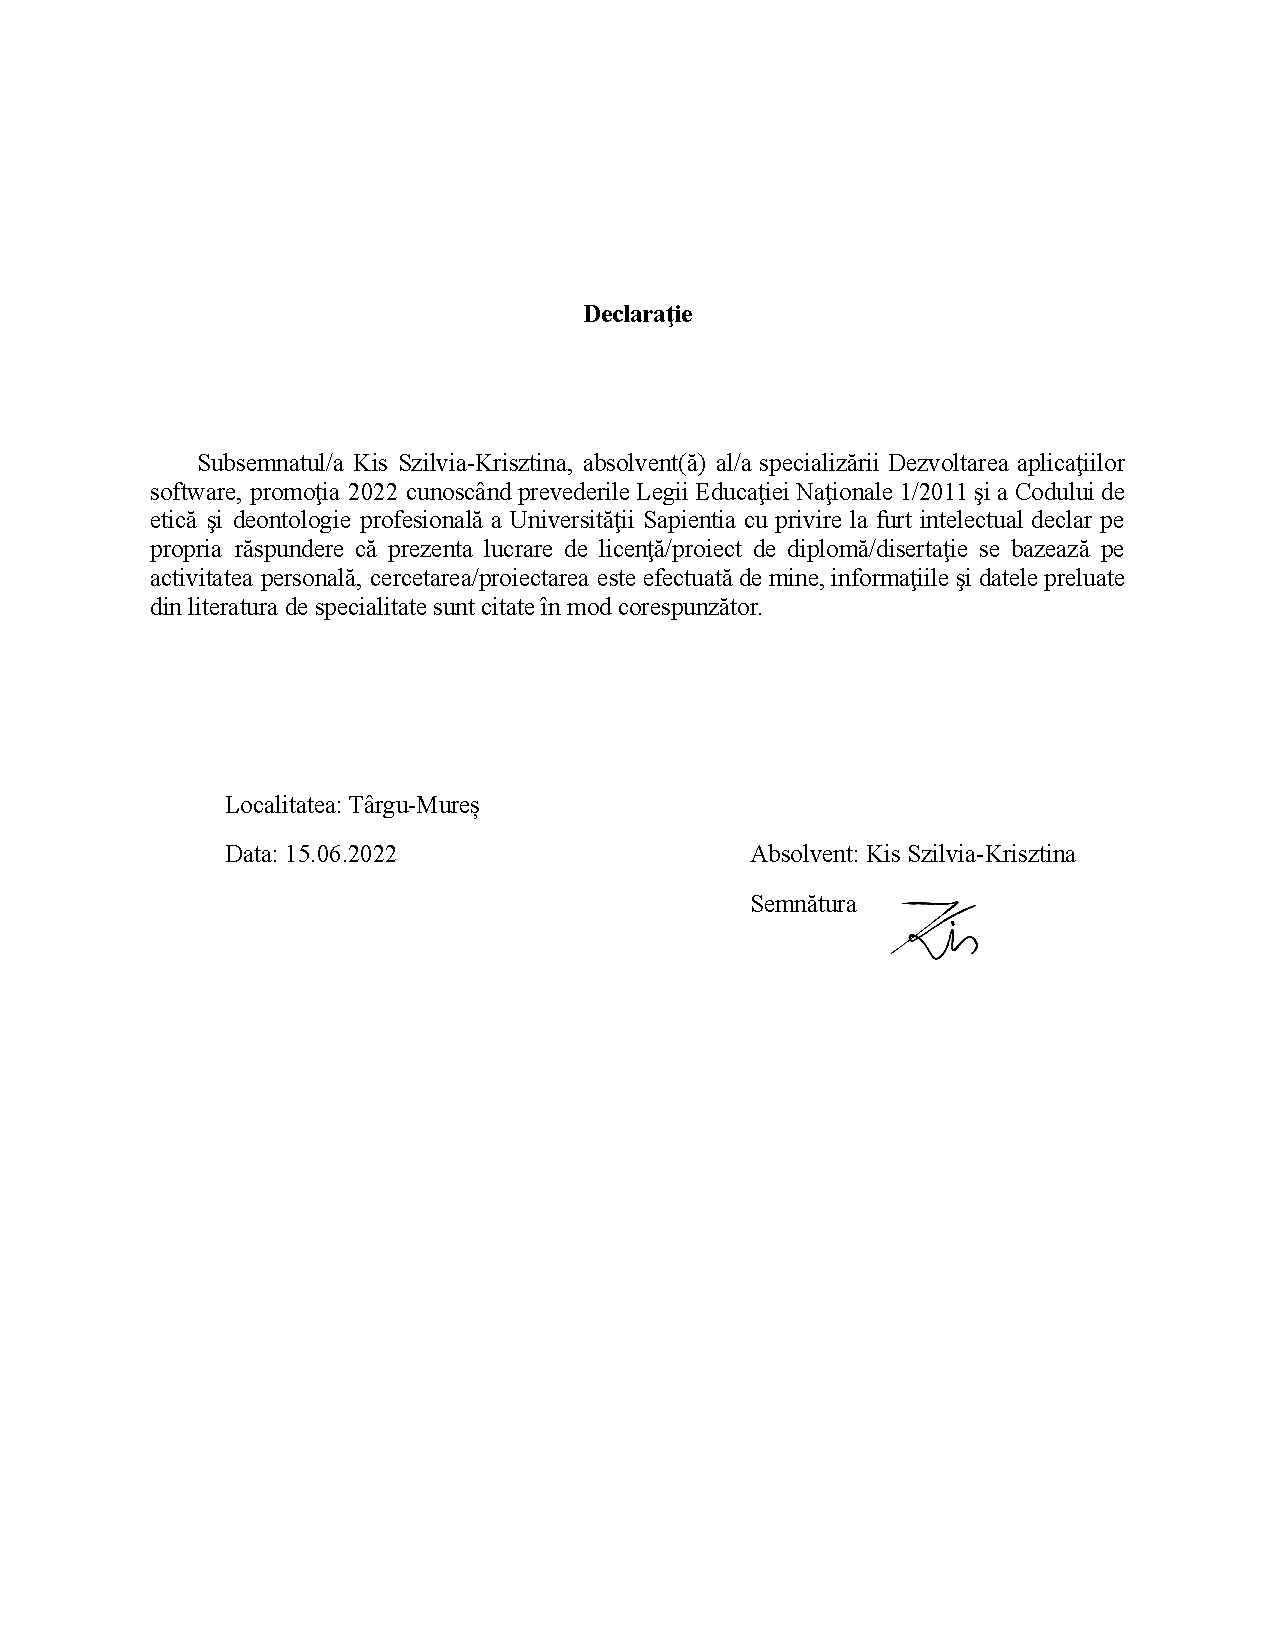
\includepdf[pages={1}]{content/Declaratie.pdf}
	\pagenumbering{gobble}

\selectlanguage{magyar}
\hungarianParagraph

%----------------------------------------------------------------------------
% Abstract in Hungarian
%----------------------------------------------------------------------------

\chapter*{Kivonat}

Napjainkban az egyetemek többsége még mindig a hagyományos  módszereket használja a tanórák során a hallgatók jelenléteinek menedzselésére. Ezen módszerek legnagyobb hátránya, hogy kicsit sem hatékonyak, illetve utólag a jelenléti ívek legtöbb esetben nem érhetőek el a diákok számára. Ugyancsak hátrányként említhető az is, hogy a később érkező diákok megzavarják az órát a procedúra elvégzése során.

A projekt célja egy korábban megvalósított jelenlétkezelő szoftverrendszer hibáinak kiküszöbölése, ugyanakkor az azonosító modul lecserélése, aminek következtében rendszerünk megbízhatóbbá, gyorsabbá és robusztusabbá válik. 

A kidolgozott rendszer sajátossága, hogy a diák részéről nem szükséges semmiféle beavatkozás a jelenléte igazolására, csupán egy arcfelismerő kamera előtt kell elsétáljon. Ennek következtében az arcfelismerő algoritmus segítségével azonosítva lesz, valamint egy életszerűség-érzékelő algoritmus biztosítja a rendszer megbízhatóságát. Ugyanakkor lehetősége van a fejlesztett mobilapplikáció letöltésére, ahol saját jelenléteit tudja követni.

Ennek tekintetében a rendszer három alappillérből áll: a jelenlétkezelő modul, melynek alkalmazásával a diák azonosítva lesz, jelenléte pedig bekerül az adatbázisba. Mindemellett a korábbi rendszer két eleme a Tanár és Diák alkalmazás kisebb változtatásokkal ugyan de továbbra is betölti szerepét. Ezáltal mind a tanárnak, mind pedig a diáknak lehetősége van a jelenlétek követésére, illetve a tanár kezében a lehetőség, hogy mindezeket kimentse.

Az applikációk fontos szerepet játszanak a tanár-diák kapcsolattartás megkönnyítésében, így a jelenlétek utánkövetésén kívül továbbra is a választható opciók között szerepel az e-mail küldés, naptáresemény létrehozása, illetve a Google tanterembe való belépés lehetősége is.

A diákok azonosítására alkalmazott modul futtatásához egy számítógépre, valamint az applikáció használatához Android operációs rendszerrel rendelkező telefonokra van szükség. A használt adatbázis felhő alapú, amely könnyebb elérést és átjárhatóságot biztosít a különböző modulok között.


\vspace*{2cm}

\noindent \textbf{Kulcsszavak:} jelenlét, azonosítás, arcfelismerés, életszerűség-érzékelés, Android alkalmazás
\vfill
\selectlanguage{romanian}

%----------------------------------------------------------------------------
% Abstract in Romanian
%----------------------------------------------------------------------------
\chapter*{Rezumat}

În zilele noastre majoritatea universităților urmărește metoda veche în decursul orelor pentru a gestiona prezența studenților. Dezavantajul acestor metode este că nu sunt deloc eficiente, respectiv foaia de prezență nu rămâne accesibil pentru studenți. De asemenea faptul că studenții care întârzie, deranjează ceilalți colegi cu această procedură poate fi menționată iarăși ca un dezavantaj.

Scopul proiectului este de a elimina erorile dintr-un sistem software anterior dezvoltat, în același timp înlocuirea modulului de identificare, ceea ce face sistemul nostru mai fiabil, mai rapid și eficient. 

Particularitatea sistemului dezvoltat este că studenții nu au nevoie de nici o intervenție pentru a verificarea prezenței, trebuie doar să treacă în fața unei camere de recunoaștere facială. Ca urmare, acesta va fi identificat cu ajutorul algoritmului de recunoaștere facială, iar algoritmul de detectare a vitalității asigură fiabilitatea sistemului. In acelasi timp aveți opțiunea de a descărca aplicația mobilă dezvoltată, de unde se va putea urmări prezența.

În acest sens, sistemul este format din trei piloni de bază: modulul de management al prezenței, datorită cărui studentul va fi identificat, iar prezența acestuia va fi introdusă în baza de date. In plus
cele două elemente al sistemului anterior dezvoltat  Profesor și Student, deși cu modificări minore continuă să-și îndeplinească rolul. Drept urmare, atât profesorul, cât și elevul au posibilitatea de a  urmări prezența la curs, iar profesorul are posibilitatea de a salva informațiile. 

Aplicațiile joacă un rol important în facilitarea contactului profesor-elev, și pe lângă faptul că  poate deține evidența prezenței, râmăn valabile și celelalte opțiuni cum ar fi trimiterea unui e-mail, crearea unui eveniment și posibilitatea de a intra în Google Classroom.

Pentru a rula modulul de identificare a elevului avem nevoie doar de un calculator, si totodata pentru a utiliza aplicația, aveți nevoie de telefoane cu sisteme de operare Android.
Baza de date utilizate este bazat pe un cloud, ceea ce reprezintă un acces mai ușor pentru permeabilitatea între module.


\vspace*{2cm}


\noindent \textbf{Cuvinte de cheie:} prezență, identificare, recunoaștere a feței, detectare a realității, aplicație Android

\vfill
\selectlanguage{english}
%\englishParagraph

%----------------------------------------------------------------------------
% Abstract in English
%----------------------------------------------------------------------------
\chapter*{Abstract}

Present-day educational system is far behind the modern era in some aspects. The majority of universities even today’s digital world still use traditional, paper based methods for managing student attendances. One of the biggest disadvantage of these methods is the lack of effectiveness. Furthermore, the later arrival students may disrupt the class while performing this procedure, not mentioning the absence of the records available for students afterwards.

The purpose of this project is to eliminate the previously implemented management software’s errors. Moreover, making it more reliable, faster and robust by replacing the identification module with a state-of-the-art neural network based facial image recognizer.

The system’s superiority is that the identification requires no special user interaction. Students only have to walk in front of a facial recognition camera. An appropriate facial recognition algorithm identifies the user, synchronously a liveness detection algorithm ensures the reliability of the system. In addition, users have the possibility to follow the attendance history.

The system consists of three main pillars. The attendance management module is responsible for identifying students and logging their data into the database. The existing Student and Teacher modules’ role remained the same, although contain minor changes. Appropriately both teachers and students have the opportunity to track attendances, while teachers can also export data.

The application takes an extensive role facilitating student-teacher contact. For this reason supplementary features added to the system, such as sending notification e-mails, creating calendar events and embedding Google Classroom access.

The facial recognition module requires a desktop environment, while the application runs on the Android operation system. The target database is cloud-based which contributes to an easier access and interoperability between the distinct modules.

\vspace*{2cm}

\noindent \textbf{Keywords:} attendance, identification, face recognition, liveness detection, Android application 

\vfill
\dolgozatnyelve
\defaultParagraph
 
% Tartalomjegyzek
%~~~~~~~~~~~~~~~~~~~~~~~~~~~~~~~~~~~~~~~~~~~~~~~~~~~~~~~~~~~~~~~~~~~~~~~~~~~~~~~~~~~~~~
	\pagenumbering{arabic}
	\setcounter{page}{9}
	\tableofcontents\vfill

% A diplomadolgozat lenyegi resze
%~~~~~~~~~~~~~~~~~~~~~~~~~~~~~~~~~~~~~~~~~~~~~~~~~~~~~~~~~~~~~~~~~~~~~~~~~~~~~~~~~~~~~~

% ajánlott külön file-okba írni az egyes fejezeteket, ugyanis úgy jobban át lehet látni.


    
	%----------------------------------------------------------------------------
\chapter{Bevezető}%\addcontentsline{toc}{chapter}{Bevezető}
%----------------------------------------------------------------------------

Egy 21. századi jelenség, hogy az embert digitális eszközök veszik körül az élet minden területén, ami a rohamosan fejlődő technikának köszönhető. Nincs ez másképp az oktatás területén sem. Nagyon fontos, bár nehéz vállalás, hogy a tanárok és a tanügyi rendszer is állja a sarat a modern technológiai kihívásokkal szemben.

Az új technológiai kihívásokkal szemben legkönnyebben a felsőoktatási intézmények, az egyetemek tudják felvenni a versenyt. Ez annak köszönhető, hogy az egyetemek és hallgatóik talán a lehető legegyszerűbben és leggyorsabban tudnak igazodni a változásokhoz, és a tapasztalatok azt mutatják, hogy törekednek is a fejlődésre, korszerű és új módszerek bevezetésével.

Ennek ellenére, még mindig sok az olyan tanintézmény, ahol a hagyományos jelenlétkezelő módszereket alkalmazzák az órák során. Ide tartozik a papírra való névsorírás, amikor a diákok maguk írják fel neveiket, de hasonló módszer az is amikor névsorolvasás történik, és a tanár végzi el a jelenlétkezelés adminisztratív részét. 
Egyöntetűen állíthatjuk, hogy ezen módszerek egyike sem hatékony és megbízható, mivel a diákok részéről könnyen átjátszható, ennek kiküszöbölésére pedig még több intézkedésre van szükség, ami növeli az erre szánt időkeretet. Emellett pedig az utánkövetés lehetősége egészen minimális, valamint többletmunkával jár a tanár részéről ezen adatok karbantartása. Mindegyik módszerre igaz az, hogy időtakarékosság szempontjából a lehető legrosszabbul teljesítenek. Az oktatásra szánt időből veszítünk el ezáltal hasznos perceket, amit a fejlődésre kellene fordítani. Fontos, hogy minden téren törekedjünk az ilyen és ehhez hasonló adminisztratív feladatok digitalizálására.

A fő kérdés, hogy mit kell szem előtt tartanunk egy jelenlétkezelő alkalmazás kivitelezése során? A válasz egyszerű: legyen hatékony, megbízható, könnyen kezelhető és mindenki számára hozzáférhető.

Kivitelezés szempontjából már nehezebb dolgunk van, hiszen fontos, hogy olyan rendszert alakítsunk ki, ami olyan szoftver és hardver eszközöket igényel, melyek könnyen elérhetőek és anyagi vonzatuk sem jelentős. Erre a legjobb megoldás az okostelefon, mint a rendszer részét képező eszköz bevonása, illetve a hiteles adatok tekintetében a biometrikus azonosítás alkalmazása. Emellett ami szintén nagyon fontos, hogy a rendszer használata érdekében a hallgató nem lehet kényszerítve arra, hogy rendelkezzen az eszközzel, illetve hogy a tanórák során használja azt. 

Számos irodalmi tanulmányban beszélnek arról, hogy hogyan és milyen számítástechnikai eszközöket vesznek igénybe az oktatás lebonyolítása során. Nagyon sok próbálkozás született már digitalizált jelenlétkezelő alkalmazás megvalósítására, amelyek más-más eszközt használnak a hatékonyság, biztonság és gyorsaság érdekében. Ilyen eszköz például RFID, ami bár hatékony, viszont kijátszhatósága megkérdőjelezhető, illetve ennek alkalmazása egy plusz eszközt igényel, amelyet minden diák számára biztosítani kell. 

A dolgozat során az ehhez hasonló problémákra keresünk megoldást, valamint ennek keretein belül szeretnénk megvalósítani azt a jelenlétkezelő rendszert, amely megfelel a technológiai elvárásoknak. 

Mivel sok esetben fontos az órai jelenlétek során egy meghatározott mennyiség megléte, nagyon fontos az is, hogy a hibalehetőségeket a minimálisra csökkentsük, ugyanakkor a megbízhatóság szempontjából a lehető legjobb megoldásra törekedjünk. Figyelembe kell vennünk azt is, hogy amennyiben lehet minimalizáljuk a beavatkozások szükségességét úgy a tanár mint a diák részéről. 

A modern jelenlétkezelő alkalmazás elvárt funkcionalitása a jelenlétek utánkövetésének lehetőség tanár és diák oldalon egyaránt. Ez egy olyan előnyt jelent a digitalizált megoldás részéről, amit egyik szokványos megközelítés sem tud biztosítani. Ezenkívül számos olyan előnnyel járhat, ami megkönnyíti, felgyorsítja és hatékonyabbá teszi az egyetemi órákon való jelenlétek menedzselését.

Az általunk fejlesztett élő arcfelismerés-alapú jelenlétkezelő alkalmazással szeretnénk hozzájárulni az egyetemen történő jelenlétkezelés új szintre való emeléséhez, eleget téve a felhasználók igényeinek és a technológiai elvárásoknak.

    %----------------------------------------------------------------------------
\chapter{Irodalomkutatás} \label{chapter1}
%----------------------------------------------------------------------------

A témával kapcsolatos kifejezésekre keresve a szakirodalmi cikkek sokasága között, mint például \enquote{attendance monitor}, \enquote{attendance management system}, nagyon sok elméleti és gyakorlati megvalósítás lelhető fel. Többfajta rendszert kidolgoztak már az egyetemi jelenlétkezelés problémájának megoldására, amelyek általában az alkalmazott módszerek és technológiákban különböznek egymástól. 

\section{RFID}

Az \cite{1} cikkben az RFID-t (Rádiófrekvencia-azonosítás) alkalmazzák egy jelenlétkezelő rendszer megvalósításához. Az RFID segítségével egy újfajta technológia kerül alkalmazásra az egyetemi jelenlétkezelés terén, aminek előnyei között említjük a megbízhatóságot, az időmegtakarítást és a könnyen kezelhetőséget \cite{3}.

Az RFID előnyei közé tartozik főkent az automatizált azonosítás, valamint adatgyűjtés. Az RFID technológiát már évtizedekkel ezelőtt is ismerték, azonban csak az utóbbi néhány évben kezdték el alkalmazni és továbbfejleszteni minél szélesebb körben, mivel korábban a költsége volt az ami korlátozta felhasználását \cite{2}.

Az RFID rendszerek négy komponensből állnak:
\begin{itemize}
			\item RFID olvasó (RFID Reader)
			\item RFID címke (RFID tag)
			\item RFID köztes szoftver (RFID Middleware)
			\item adatbázis (Database Storage)
\end{itemize}

Az olvasó, amit más néven lekérdezőnek is nevezünk, feladata, hogy antennákon keresztül rádiófrekvenciás adatokat tud küldeni és fogadni a címkékből. Egy olvasónak akár több antennája is lehet, amelyek feladata a rádióhullámok küldése és vétele. A címke az adatokat tároló mikrochipből, egy hordozóból és egy antennából tevődik össze. Ebbe van felszerelve a chip és az antenna. Az RFID Middleware a rendszer azon része, amely megtisztítja és kiszűri a nyers RFID-értékeket. Maga az olvasótól kapja az adatokat, majd különböző módszereket alkalmaz, hogy a beérkezett adatokból csak a hasznos információkat gyűjtse be. A megtisztított rekordok, ideértve a tag-ek és az olvasó azonosítóit is, illetve a leolvasott időbélyeget, mentésre kerülnek az adatbázisba \cite{1}. Ez a mechanizmusa az RFID-t használó jelenlétkezelő rendszereknek. Összességében minden diák rendelkezik egy azonosító eszközzel, a leolvasott adatok mentésre kerülnek az adatbázisba, ahonnan bármikor megjeleníthető lesz egy adott felhasználói felületen.
A tanulmányozott cikkben említett módszer működőképes megoldást nyújt, azonban vannak olyan hátrányai, ami miatt mi nem ezt a megoldást választottuk. Hátrányai közé tartozik, hogy az RFID-t alkalmazó megoldáshoz szükség van bizonyos hardver eszközökre, amelyeknek anyagi vonzata is van, mindemellett pedig egy rögzített rendszerről beszélünk. Egyetemi szinten ez azt jelenti, hogy mind a termek, mind pedig a diákoknak rendelkezniük kell a rendszer működését biztosító eszközökkel. Amennyiben ezek az akadályok áthidalhatóak, a megoldás alkalmazható az egyetemi jelenlét hatékony kezelésére.



\section{Biometrikus azonosítás}

A biometrikus azonosítást alkalmazó rendszerek esetén az ember valamilyen egyedi sajátosságáról veszünk mintát (ujjlenyomat, retina, hang stb.), ezek kerülnek tárolásra miután digitális adattá lettek konvertálva. Az aktuális mintát fogja összehasonlítani a már meglévő mintákkal, melyek tárolva vannak az adatbázisban.
A hivatalos megfogalmazás alapján: \enquote{a biometria az alapján azonosít, ami az ember maga, nem pedig az alapján, amit tud (kód, jelszó), vagy amije van (kártya, távirányító)} \cite{5}.

\subsection{Ujjlenyomat}

A \cite{4} cikkben bemutatott megvalósítás biometrikus adatot használ fel, ujjlenyomat formájában a hallgatók azonosítására. A tárgyalt rendszer működtetéséhez nincs szükség a tanár beavatkozására, illetve mivel maga az eszköz hordozható formában lett kivitelezve, amely akkumulátorral üzemeltethető, nincs helyhez kötve, így akár óraközben is tudja jelezni a hallgató órai jelenlétét. A megoldás egyszerű: a diák megérinti az érzékelő felületet, és az eszköz feladata begyűjteni a ujjlenyomatokat. Az információkat egy USB csatlakozón keresztül lehet csatlakoztatni a számítógéphez. A tanár számára rendelkezésre áll egy felhasználói felület, ahol az eszközt és a jelenléteket is az ellenőrzése alatt tudja tartani.

A rendszer fő komponense a ujjlenyomat olvasó modul, ezenkívül egy Real Time Clock-ból (RTC), a gombokból és a grafikus folyadékkristályos kijelzőből (GLCD) áll, és mindezt egy mikrovezérlő irányít. A kijelző az aktuális diák jelenléti állapotának megjelenítéséért felel. Ezek az állapotok a sikeres párosítás, nem sikeres, vagy már jelentkezett. \cite{4}.
Ez az eszköz meghatározott ideig képes tárolni az adatokat, csak akkor kell számítógéphez csatlakoztatni, ha egy összesítést szeretnénk kapni, esetleg ki szeretnénk menteni azokat.
Elmondhatjuk, hogy a rendszer eleget tesz a hatékony jelenlétkezelés elvárásainak, mindemellett megbízhatóbb megoldás, mint az RFID-val történő megközelítés, mivel így biztosított az, hogy adott diák csak saját jelenlétét tudja igazolni, ellenben amikor egy eszközzel kell ezt megtenni, ami könnyen adatható és felhasználható más személyek által is.

Az említett rendszernek több előnyét is megemlíthetjük: gyorsaság, időtakaréskosság, megbízhatóság. Ezek mellett egyik legnagyobb előnye, hogy az óra folyamán történő jelenlétek bevitele nem igényli a tanár beavatkozását és nem zavarja az óra menetét.

Hogy miért nem alkalmaztunk mégsem ujjlenyomat alapú azonosítást a saját rendszerünkben, egyszerű magyarázata van: mint minden biometrikus azonosítást lehetővé tévő rendszer különleges hardver eszközöket igényel, amelyek beszerzése jelentős pénzösszegbe kerül, illetve higiéniai szempontból is kérdéses, hogy mennyire megfelől ezt a megoldást használni egy nagy létszámú egyetemi közösségben \cite{6}. 

\subsection{Arcfelismerés}

A \cite{7} cikkben egy szintén biometrikus azonosítást bemutató alkalmazásról lehet olvasni. Egy olyan rendszert mutatnak be, ahol arcfelismerést használnak a diákok azonosításra az órai jelenlétek követése végett. A rendszer azonosítani tudja a diákot digitális képből vagy videóforrásból is.

Az azonosításnak két fő mozzanata van:
\begin{itemize}
			\item Az arc körvonalának megkeresése és a háttér eltávolítása.
			\item Az azonosított arcot összehasonlítja az adatbázisban előzőleg eltárolt \enquote{mintákkal}. 
\end{itemize}
Az összehasonlítási eljárásra két matematikai transzformációkon és analízisen alapuló eljárást alkalmaznak. Az egyik az arcról készült képet vizsgálja, a másik pedig az arc különböző részeit keresi meg, mint az orr, szemek, száj, stb. azok egymástól mért távolságát és elhelyezkedését \cite{6}.

A tanulmányozott cikkben egy hagyományos arcfelismerő rendszer lett megvalósítva. Először detektálja az arcot, azután felismeri/azonosítja.
Megtörténik az érdekeltségi kör kiválasztása, ami azt jelenti, hogy körülvágja a megtalált arcot, eltávolítja a hátteret, majd összehasonlítja az adatbázisban szereplő adatokkal. 

A rendszer fő alkotóeleme a kamera, ez felel az osztálytermi kép rögzítéséért, amik továbbítva lesznek a képjavító részhez. Javítás után a detektáló és felismerő algoritmusokon megy keresztül, majd miután megtörtént az azonosítás a jelenlét bekerül az adatbázisba. Ami a rendszer legnagyobb pozitívuma, hogy egyszerre több arcot detektál a képről, valamint össze van kötve az órarenddel, így meg tudja határozni a tantárgyat, az adott osztálycsoportot, a dátumot és az időt is.
Mivel csak egy gombnyomásba kerül a tanárnak a jelenlét rögzítése, nagyon sok idő és adminisztratív munka spórolható meg. A diákok jelenléteihez hozzáférhetnek ők maguk, a tanárok, de akár a szülők is.

A képek készítése folyamatos, több kép is készül, hogy biztosan minden arc detektálva legyen a teremben.
Hogy a hibás detektálást a minimálisra csökkentsék, a bőr szerinti osztályozást alkalmazzák, azaz a bőr képpontjait megtartják, és a kép többi része fekete színt kap \cite{7}. 

Az ujjlenyomat általi azonosítást használó rendszerrel szemben a tárgyalt megoldás sokkal több előnnyel rendelkezik. Fő előnye (főleg a vírusos időszakokat szem előtt tartva), hogy nincs fizikai érintkezés a diák és az eszköz között. Az is kiemelkedő előnynek számít, hogy egyszerre több arcot is tud detektálni, így sokkal hatékonyabb az előző megoldással szemben, ez azonban akár hátránya is lehet a rendszernek.

Mindezek mellett komoly hátrányt jelenthet a rendszer esetén, ha egy diák arca nem lesz látható az óra folyamán, így a jelenléte nem kerül rögzítésre. Ami méginkább gondot okoz az a jogi és adatvédelmi problémák. Ezt azt jelenti, hogy jogi következményei lehetnek, ha a diák arcának detektálása az előzőleges beleegyezése nélkül történt. Mindemellett a rendszer működését befolyásolhatják a különböző fényviszonyok, és viszonylag egyszerűen \enquote{átverhető} egy fotóval \cite{8}.


\section{Következtetés}

Számos cikk között kutatva a témában, sikerült levonni olyan következtetéseket, amelyek alátámasztják egy hatékony és megbízható rendszerrel szembeni alapelvárásokat.
Ezen következtetések alapján kimondhatjuk, hogy egy hatékony jelenlétkezelő rendszer a következő elvárásoknak kell eleget tegyen:
\begin{itemize}
	\item {Azonosítás: egyedi és nehezen kijátszható azonosító.}
	\item {Eszköz: mindenki számára elérhető és költséghatékony.}
	\item {Adattárolás: naprakész, valós idejű adatbázis.}
	\item {Gyorsaság:  helyesen detektálni és rögzíteni a diák jelenlétét minél rövidebb idő alatt.}
\end{itemize}

A jól működő rendszer fő tulajdonságai: egyszerűség, gyorsaság, hatékonyság. Ezek a legfontosabb dolgok, amit egy konzisztens, egyetemi jelenlétkezelő alkalmazás esetében szem előtt kell tartanunk.

Következtetésként elmondható, hogy egy jól használható jelenlétkezelő rendszer létrehozásakor néha olyan kompromisszumokra van szükség, amely során egyik tulajdonság alulmaradása mellett egy másik felerősödik. Erre jó példa a biztonság és a könnyen használhatóság közötti egyensúly megtalálása. Nagyon sok esetben áldozatokra van szükség, ahogy esetünkben is, egy biometrikus adat kerül vételezésre, azaz a diák arca, így ez sok helyen GDPR problémákba ütközhet. Ugyanakkor ennek előnye, hogy nem lehet kijátszani a rendszert. Áldozatot jelent az is, hogy egy mobilapplikáció áll a felhasználó rendelkezésére, így annak használathoz elengedhetetlen a saját eszközére való telepítés.

A kérdés csak az, hogy mekkora lehet az áldozat, amit annak érdekében hozunk, hogy egy biztonságos, gyorsan és egyszerűen kezelhető rendszert tudjunk megalkotni.










    %----------------------------------------------------------------------------
\chapter{Célkitűzések} \label{chapter2}
%----------------------------------------------------------------------------

A dolgozat célja a modern technológiai elvárásoknak megfelelő jelenlétkezelő rendszer megvalósítása, amely kielégíti rohamosan fejlődő digitális világunk elvárásait mint megvalósítás, mint pedig használhatóság szempontjából. 
Egy olyan rendszer kidolgozása a cél, amely növeli az órai jelenlétkezelés hatékonyságát. Ez elsősorban időhatékonyságot és gyors működést feltételez, mivel az a cél, hogy az óra időtartamából a lehető legkevesebbet tegye ki a jelenlétek menedzselése.

A rendszer megvalósítása során külön figyelmet kell szentelnünk annak, hogy használata olyan erőforrásokat igényeljen, ami mindenki számára elérhető, mellőzve a jelentős anyagi vonzatát. Mindezt figyelembe véve jutottunk arra a következtetésre, hogy az okostelefon jelenti a leghatékonyabb eszközt a rendszer használatára, mivel elmondható, hogy már minden diák rendelkezik vele. A fő modul, ami a diákok detektálását és azonosítását végzi legyen minél kevesebb beavatkozást igénylő megoldás, ami gyors és hatékony is egyben.

Mindezek mellett fontos cél az is, hogy a jelenléteket ne csak rögzítsük, hanem elérhetővé is tegyük a tanárok és diákok számára, hogy azok bármikor megtekinthetőek legyenek. A megtekinthetőség mellett az is nagyon fontos, hogy a tanárnak lehetősége legyen lementeni a jelenléteket, tantárgyakra lebontva, választható formátumban.

A rendszer kiegészítő funkcionalitásaként, az online oktatási folyamatokat egyszerűsítő eszközöket is szeretnénk elérhetővé tenni az alkalmazáson belül. Ez azt jelenti, hogy minden tantárgyhoz, ami megjelenik a rendszerben, rendelünk egy Google tantermet (Google Classroom), így azonnal elérhetővé válik, amennyiben a tanár használni szeretné. Az e-mail küldés, mint kiegészítő funkciónak is hasznos szerepe van az online világ hatékony működésében, így ezen folyamat leegyszerűsítése végett implementálunk egy olyan opciót, ami lehetővé teszi a tanár és diák számára az e-mail küldést. Abban különbözik a sima e-mail küldési lehetőségtől, hogy a diáknak nem kell tudnia a tanár e-mail címét, kiválasztva a nevét máris tud üzenetet küldeni. A tanár esetében ez a plusz azt jelenti, hogy egyszerűen tud csoportos e-mailt küldeni méghozzá a szak és tantárgy kiválasztásával.

Amennyiben a célkitűzéseinket sikerül megvalósítani, már egy olyan jelenlétkezelő rendszert tudunk biztosítani, ami megállja a helyét az egyetemi szférában is, kiemelve a hatékonyságot, időspórlást és a gyors működést. Emellett a továbbfejlesztési lehetőségek tárháza is végtelen, amelyet a jövőben az igények és visszajelzések alapján szeretnénk megvalósítani.




    %----------------------------------------------------------------------------
\chapter{Korábbi megoldás rövid bemutatása} \label{chapter3}
%----------------------------------------------------------------------------

A jelenlegi dolgozatom alaptémáját a 2 évvel ezelőtti licensz dolgozatom adta, miszerint az egyetemen zajló jelenlétkezelési mechanizmust szeretnénk korszerűsíteni. Korábbi megoldásom QR kód alapú megoldás volt, ami csupán egy okostelefon meglétét igényelte.
A Diák alkalmazás a Tanár alkalmazással egy QR kód segítségével kommunikált, ezáltal tudta azonosítani magát a diák az egyetemi órákon. Mindkét alkalmazásnak hozzáférése volt egy közös Firebase adatbázishoz, ahol az adatok beírásra, majd lekérdezésre kerültek.

A megvalósított rendszernek két kulcsfunkcionalitása volt:

\subparagraph* {Az azonosítóként szolgáló QR kód generálása}\
\newline

A diák alkalmazás esetén generálásra került egy QR kód, ami azonosítóként szolgált. Az azonosító tartalmazta a diák szakját, a nevét, a Neptun azonosítóját, és a biztonság növelése érdekében egy egyedi eszközazonosítót is.
Mivel az előzőleges regisztráció során a diák személyes adatai bekerültek az adatbázisba, csupán lekértük ezeket az adatokat a QR kód generálásához.


\subparagraph* {QR kód szkennelése a jelenlét rögzítéséhez}\
\newline

A diák azonosítására szolgáló QR kód értelmezése a Tanár alkalmazás segítségével történt. Ezen folyamat eredménye, hogy az adott diák jelenléti adati bekerülnek az adatbázisba, amely által igazolva lesz jelenléte az aktuális órán. 
Maga a szkennelés egy gombnyomásra történik, amely által megnyílik a kamera, és a QR kód fölé tartva feldolgozza az abba kódolt adatokat.
Az azonosítás mellett az tanár alkalmazás lehetővé tette a korábbi jelenlétek megtekintését, de ugyanakkor lehetőséget adott a jelenlétek kimentésére is különböző formátumokba, amit a Google Apps script biztosított. A mobilalkalmazáson keresztült került meghívásra az említett szkript, ami lehetővé tette a jelenlétek kimentését táblázat formájában a felhasználó által kiválasztott formátumban.

A kivitelezett megoldás jobb szemléltetése érdekében az alábbi ábrán látható a rendszer architektúrája:


\begin{figure}
	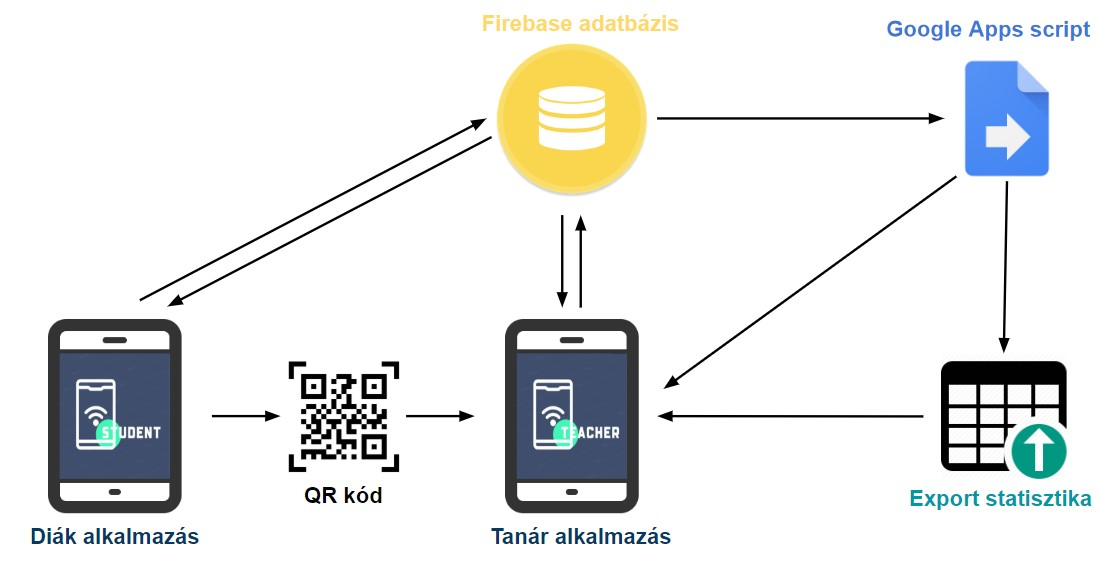
\includegraphics[width=\textwidth]{figures/architecture2.jpg}
	\caption{Az előző rendszer architektúrája}
\end{figure}

\newpage


Amint azt említettem a hallgató azonosítására szolgáló QR kód létrehozása a Diák alkalmazás feladata volt. Emellett szükséges volt egy regisztrációra és belépésre az alkalmazás funkcionalitásának igénybevételéhez, ezt követően jött létre az azonosító, illetve vissza lehetett nézni a korábbi jelenléteket. Kiegészítő funkciók közül az e-mail küldés, Neptunba és Classroom-ba való belépés volt elérhető. Mindezeket a ~\ref{fig:stud1} ábra szemlélteti.

A Tanár alkalmazáson belül elérhetőek voltak a következő funkcionalitások: regisztráció és bejelentkezés, új jelenlétek hozzáadása, korábbi jelenlétek megtekintése, jelenlétek exportálása, illetve ugyanúgy az e-mail küldési lehetőség, naptáresemény létrehozása, valamint a Google Classroom-ba történő belépés.

A Tanár applikáció három legfontosabb funkcionalitása került megjelenítésre a ~\ref{fig:teach1} ábrán.



\begin{figure}
	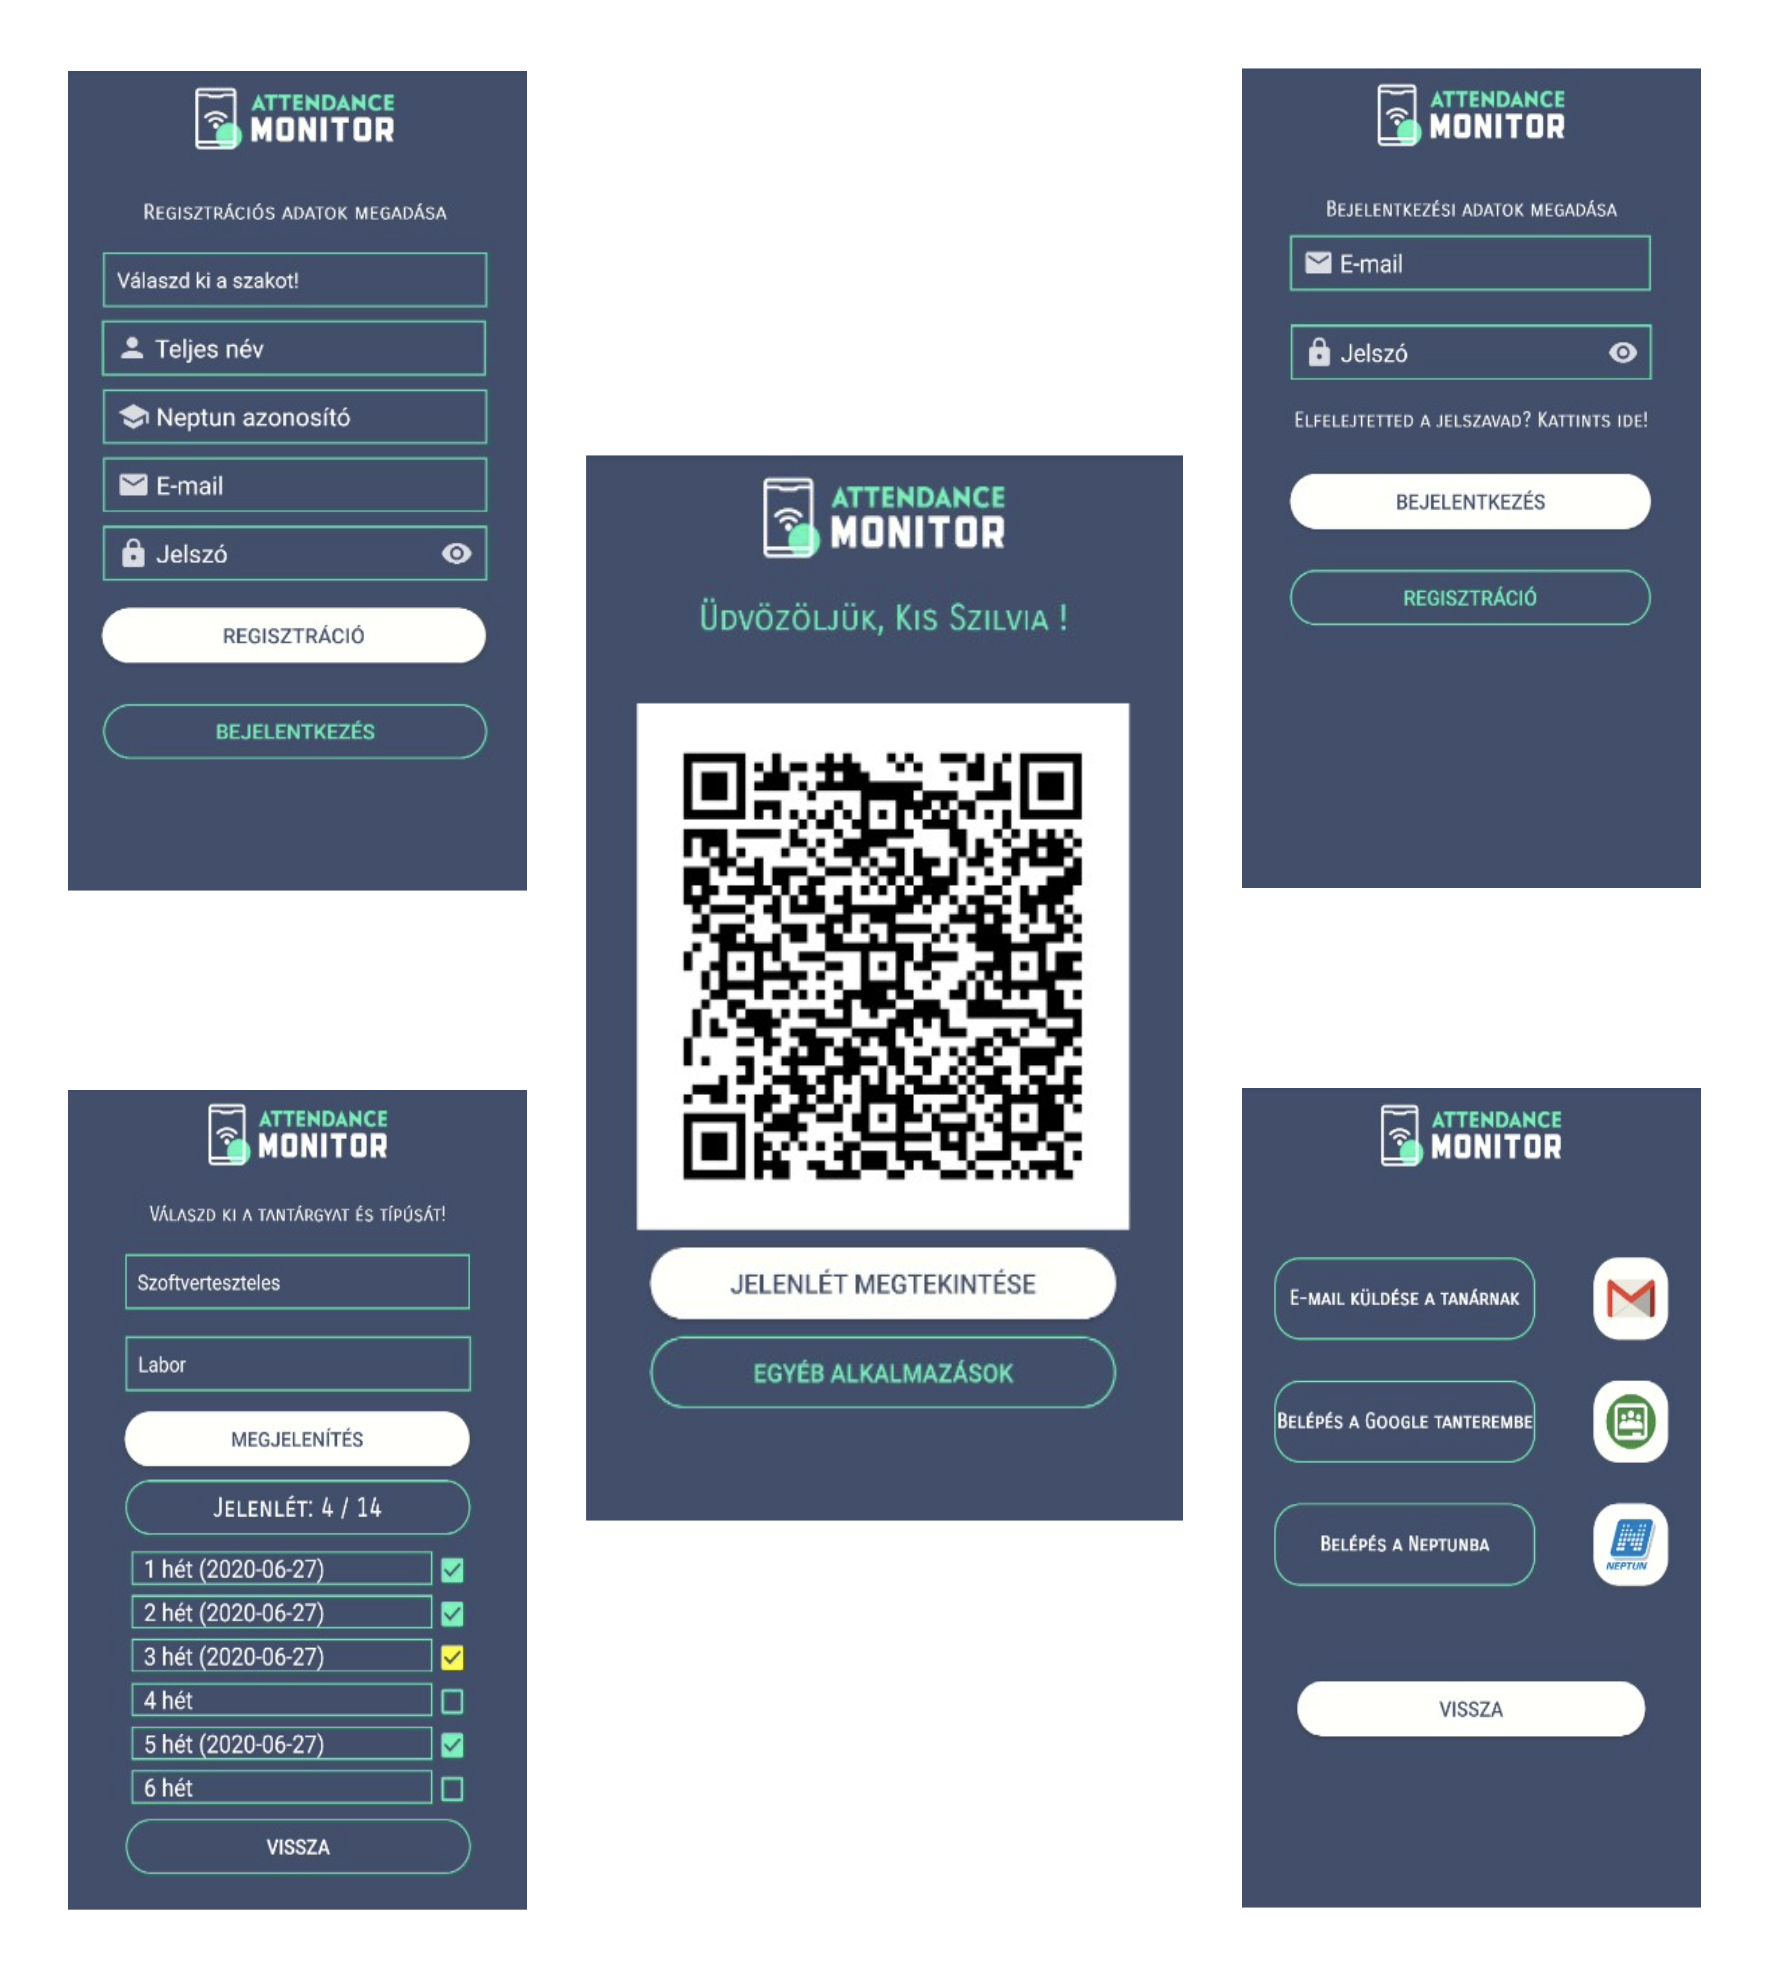
\includegraphics[width=\textwidth]{figures/stud1.png}
	\caption{Diák alkalmazás funkcionalitásai}
	\label{fig:stud1}
\end{figure}

\begin{figure}
	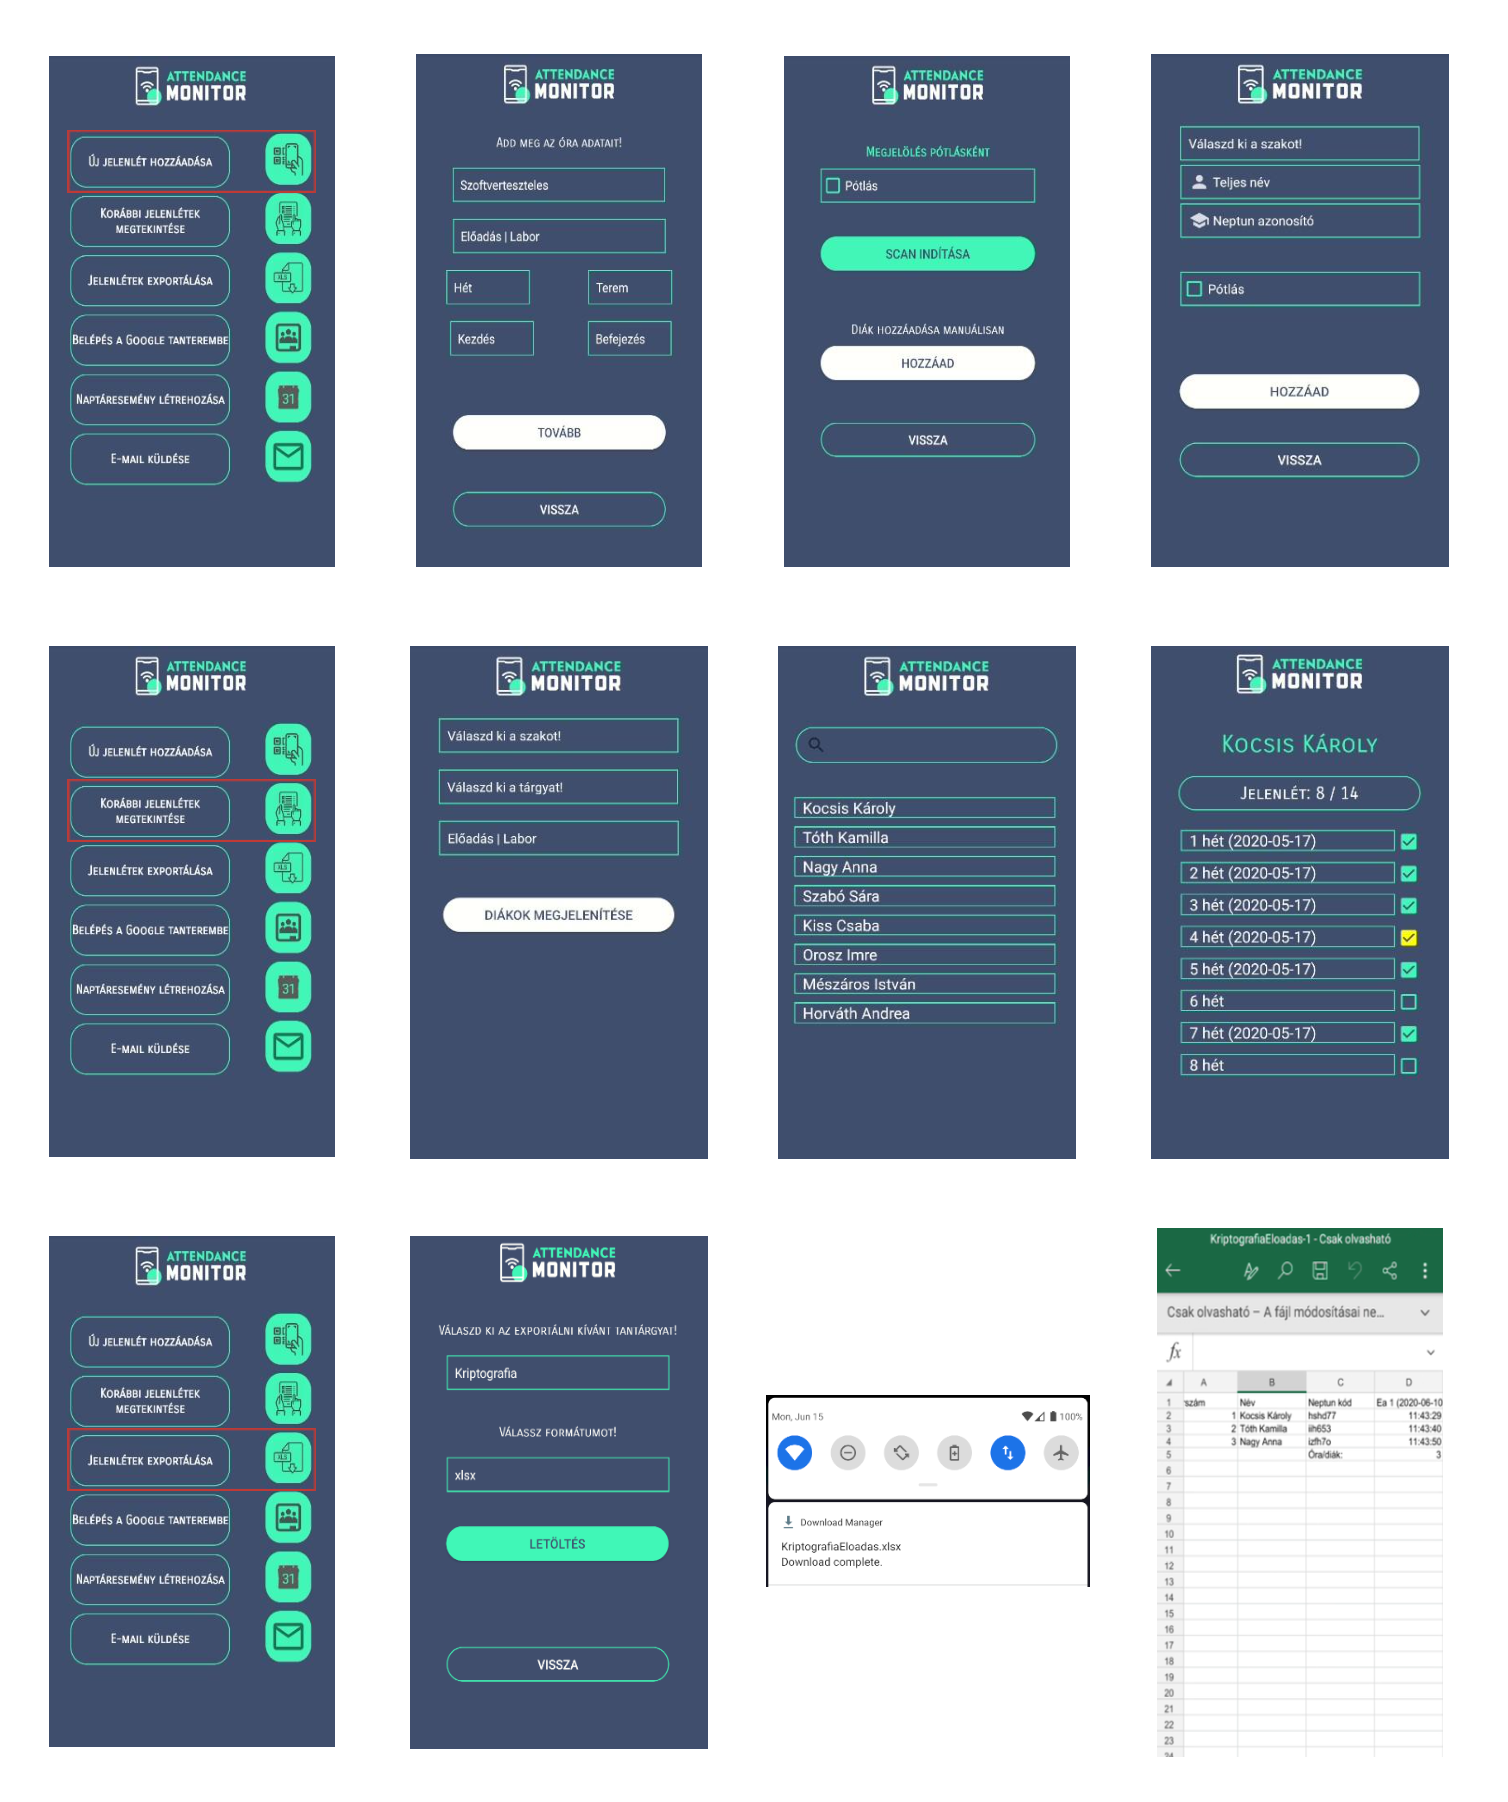
\includegraphics[width=\textwidth]{figures/teach1.png}
	\caption{Tanár alkalmazás funkcionalitásai}
	\label{fig:teach1}
\end{figure}
    %----------------------------------------------------------------------------
\chapter{Konferencia tapasztalatok} \label{chapter4}
%----------------------------------------------------------------------------

Amint azt korábban említettem, dolgozatom alaptémáját a korábbi licenszdolgozatom adta. A \textit{Jelenlétkezelő alkalmazás} című projektemmel részt vettünk a 
\href{https://mtdk.tmd.ro/index.php/site/page/?p=21}{XXII. Műszaki Tudományos Diákköri Konferencián}, alkalmazott informatika tagozaton, ahol II. helyezést értünk el. Emellett sikerült bemutatnunk a dolgozatot a \href{https://ojs.emt.ro/enelko-szamokt/article/view/327/266}{XXI. Energetika-Elektrotechnika – ENELKO és XXX. Számítástechnika és Oktatás – SzámOkt Multi-konferencia} keretein belül, ahol a dolgozat alapján megírt cikk is publikálásra került.

A tudományos bizottság mindkét esetben a biztonságot, és ami még fontosabb a rendszer átjátszhatóságát boncolgatta. Ahhoz, hogy a rendszer használható legyen, illetve ne sértsen semmilyen személyi jogokat, az átjátszhatóságot feláldoztuk ennek az oltárán. Az említett rendszer nem igényelt semmiféle olyan adatot, ami GDPR problémába ütközne, működéséhez csupán egy okostelefonra volt szükség, és bár bizonyos mértékben támadható volt, tettünk némi lépést afelé, hogy a kijátszhatóság lehetőségét a minimálisra csökkentsük. Ilyen intézkedés volt például, hogy a diák azonosítására szolgáló adatok QR kód formájában kerülnek titkosításra, amelyből csak a megfelelő alkalmazással és adatfeldolgozással kerülnek feldolgozásra. Emellett a regisztrációkor elmentettük a diák által használt eszköz egyedi azonosítóját, ami ugyanúgy kódolva lett a diákot azonosító QR kódban, ezáltal minden jelentkezéskor ellenőrizhető volt, hogy ugyanarról a telefonról lépik be adott azonosítójú diák. A nagyobb biztonság elérése érdekében a Neptun azonosítókat is ellenőriztük, ezáltal tudtuk azt kiszűrni, hogy egy alkalmazáson belül csak ugyanazzal az azonosítóval rendelkező diák tudja jelezni ottlétét.

Elmondhatjuk, hogy bár megpróbáltunk minden lehetséges támadást kivédeni, még mindig vannak olyan lehetőségek, amik teret adnak a kijátszhatóságnak, ezáltal a rendszerünk kevésbé lesz megbízható. Emellett az is fontos szerepet játszik a rendszer hatékonyságát illetően, hogy a jelenlétek bevitele szükségessé teszi a tanár és diák interakcióját is, ezáltal bár a hagyományos módszernél gyorsabb, mégsem bizonyul a leghatékonyabb eljárásnak.

A kijátszhatóság és biztonság fogalmakat tekintve a bizottság szembesített minket néhány olyan kérdéssel, amelyre a jelenlegi rendszerünkkel szeretnénk választ adni, kiküszöbölve ezzel az esetleges támadási lehetőségeket.

\newpage

Néhány nagyobb kérdés köré építettük fel a megfogalmazott problémákat:

\begin{enumerate}[label=(\alph*)]
    \item Hogyan tudom biztosítani, hogy egy diák csak egyszer tudjon jelentkezni saját alkalmazásán belül?
    \item Hogyan tudom kiküszöbölni azt, hogy az azonosító továbbküldésével egy diák mások helyett is jelentkezni tudjon?
    \item Hogyan érhetjük el azt, hogy a hatékonyságot növelve a tanár/diák beavatkozása nélkül is megbízhatóan működjön a rendszer?
    \item Gyorsaság szempontjából hogyan lehetne javítani a rendszer teljesítményén?
\end{enumerate}

Előrevetítve a dolgozatom keretein belül megvalósított rendszer megoldásait, a fent leírt kérdésekre az alábbi megoldásokkal tudunk válaszolni:

\begin{enumerate}[label=(\alph*)]
    \item Az arcfelismerés technikáját alkalmazva egy diák csak saját maga jelenlétét tudja igazolni.
    \item Az életszerűség-érzékelést alkalmazva, amennyiben egy fotót vagy videót használnak, a rendszer kiszűri a \enquote{hamis} arcokat.
    \item A hatékonyság növelése érdekében az interakciókat minimálisra csökkentettük, a diák részéről ez megszűnt, míg a tanárnak csupán egyszer kell beállítania az óra adatait, onnantól a rendszer robusztusan, külső beavatkozás nélkül funkcionál.
    \item Az interakciók kiiktatásával a jelenlétek bevitele sokkal gyorsabb lett, ugyanakkor egyszerre akár több diákot is tudunk azonosítani, ezzel is minimálisra csökkentve az erre szánt időt.
\end{enumerate}

A jelenlegi projekt keretein belül igyekeztünk egy olyan rendszert kialakítani, ami eleget tesz a megfogalmazott elvárásoknak, megbízható, robusztus és mindazonáltal minimális beavatkozást igényel. 
    %----------------------------------------------------------------------------
\chapter{Elméleti megalapozás} \label{chapter5}
%----------------------------------------------------------------------------
A \cite{9} cikket tanulmányozva láthatjuk, hogy az elmúlt években a biometrikus azonosítási technikák tűntek legígéretesebb lehetőségként az egyének felismerésére. Ezek a technikák az egyén fizikai és viselkedési jellemzőit vizsgálják, hogy azonosítsák és megállapítsák személyazonosságát, ahelyett, hogy jelszavak, PIN-kódok, intelligens kártyák, plasztikkártyák, tokenek vagy kulcsok segítségével hitelesítenék az embereket. A jelszavakat és a PIN-kódokat nehéz megjegyezni, és kitalálhatók; a kártyák, kulcsok és hasonlók könnyen elveszíthetők, ellophatók vagy sokszorosíthatók; A mágneskártyák megsérülhetnek és olvashatatlanná válhatnak. Az egyén biológiai tulajdonságait azonban nem lehet elfelejteni, ellopni vagy hamisítani. \cite{10}
Az arcfelismerés az egyik legkevésbé tolakodó és leggyorsabb módszer, összehasonlítva más technikákkal, például az ujjlenyomat- és íriszfelismeréssel.
Az arcfelismerés számos alkalmazásban való felhasználásának köszönhetően jelentős figyelmet kapott mind a kutatói közösségek, mind a piac részéről, és egyre nagyobb igény mutatkozott olyan robusztus arcfelismerő algoritmusok iránt, amelyek képesek kezelni a valós arcképeket.

Az arcfelismerő rendszerek általában két mechanizmus valamelyike szerint működnek: 

\begin{itemize}
    \item Ellenőrzés (egy az egyhez): két arckép közötti hasonlóságot mérik.
    \item Azonosítás (egy a sokhoz): egy adott arckép és egy nagy adatbázisban lévő összes arckép közötti hasonlóság kiszámításra kerül.
\end{itemize}

Az arcfelismerés magában foglalhatja az arcél-észlelést, a szegmentálást és a lokalizációt.
Az észlelt arcképek közvetlen arcfelismerésre való használata bizonyos hátrányokkal jár. Először is, minden javítás általában több mint 1000 pixelt tartalmaz, ami túl nagy ahhoz, hogy robusztus felismerő rendszert tudjanak létrehozni. Másodszor, az arcképek különböző kameraállásokból készülhetnek, eltérő arckifejezésekkel, megvilágítással. Ezen hátrányok kiküszöbölése érdekében különböző műveleteket hajtanak végre a detektált képeken, ilyen például a méretcsökkentés, zajtisztítás, stb.
\newpage
Az általános arcfelismerő rendszer fő összetevőit a ~\ref{fig:face1} ábra szemlélteti.

\begin{figure}
	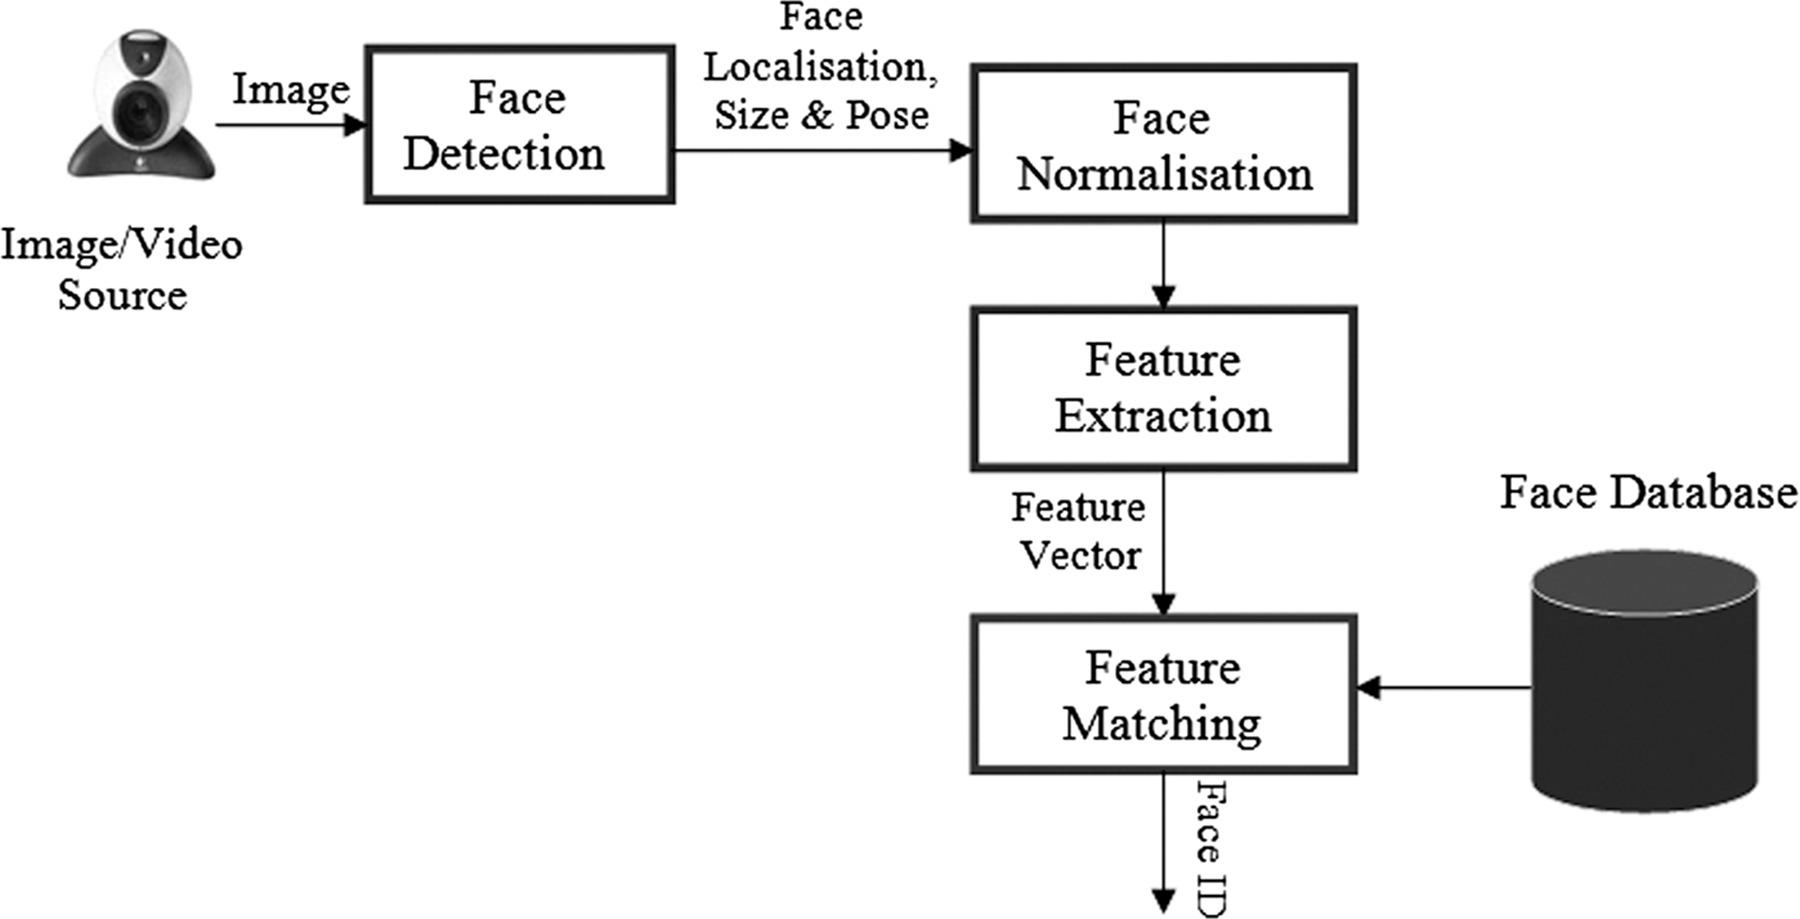
\includegraphics[width=\textwidth]{figures/facedetection_components.jpeg}
	\caption{Egy általános arcfelismerő rendszer blokkdiagramja \cite{9}}
	\label{fig:face1}
\end{figure}

\section{Az arcfelismeréssel kapcsolatos kihívások}
Általánosságban elmondható, hogy a digitális képalkotásban a jól működő arcfelismerésnek számos hátráltató tényezője ismert: váltakozó fényviszonyok, a nagy pózváltozatok, a különböző arckifejezések, a smink, az arcszőrzet változásai, az öregedés.
Valójában számos kihívás és kulcstényező van, amelyek jelentősen befolyásolhatják az arcfelismerési teljesítményt. Ezen kihívások közül néhányat a ~\ref{fig:face2} ábra szemléltet, amelyek az alábbi kategóriákba sorolhatók:

\begin{enumerate}[label=(\alph*)]
    \item Kihívások a fényviszonyok változásai miatt
    \item Kihívások a pózváltozás miatt
    \item Kihívások az öregedési változások miatt
    \item Kihívások az arckifejezés/arcstílus miatt
    \item Kihívások az eltakarás miatt
\end{enumerate}

\begin{figure}
	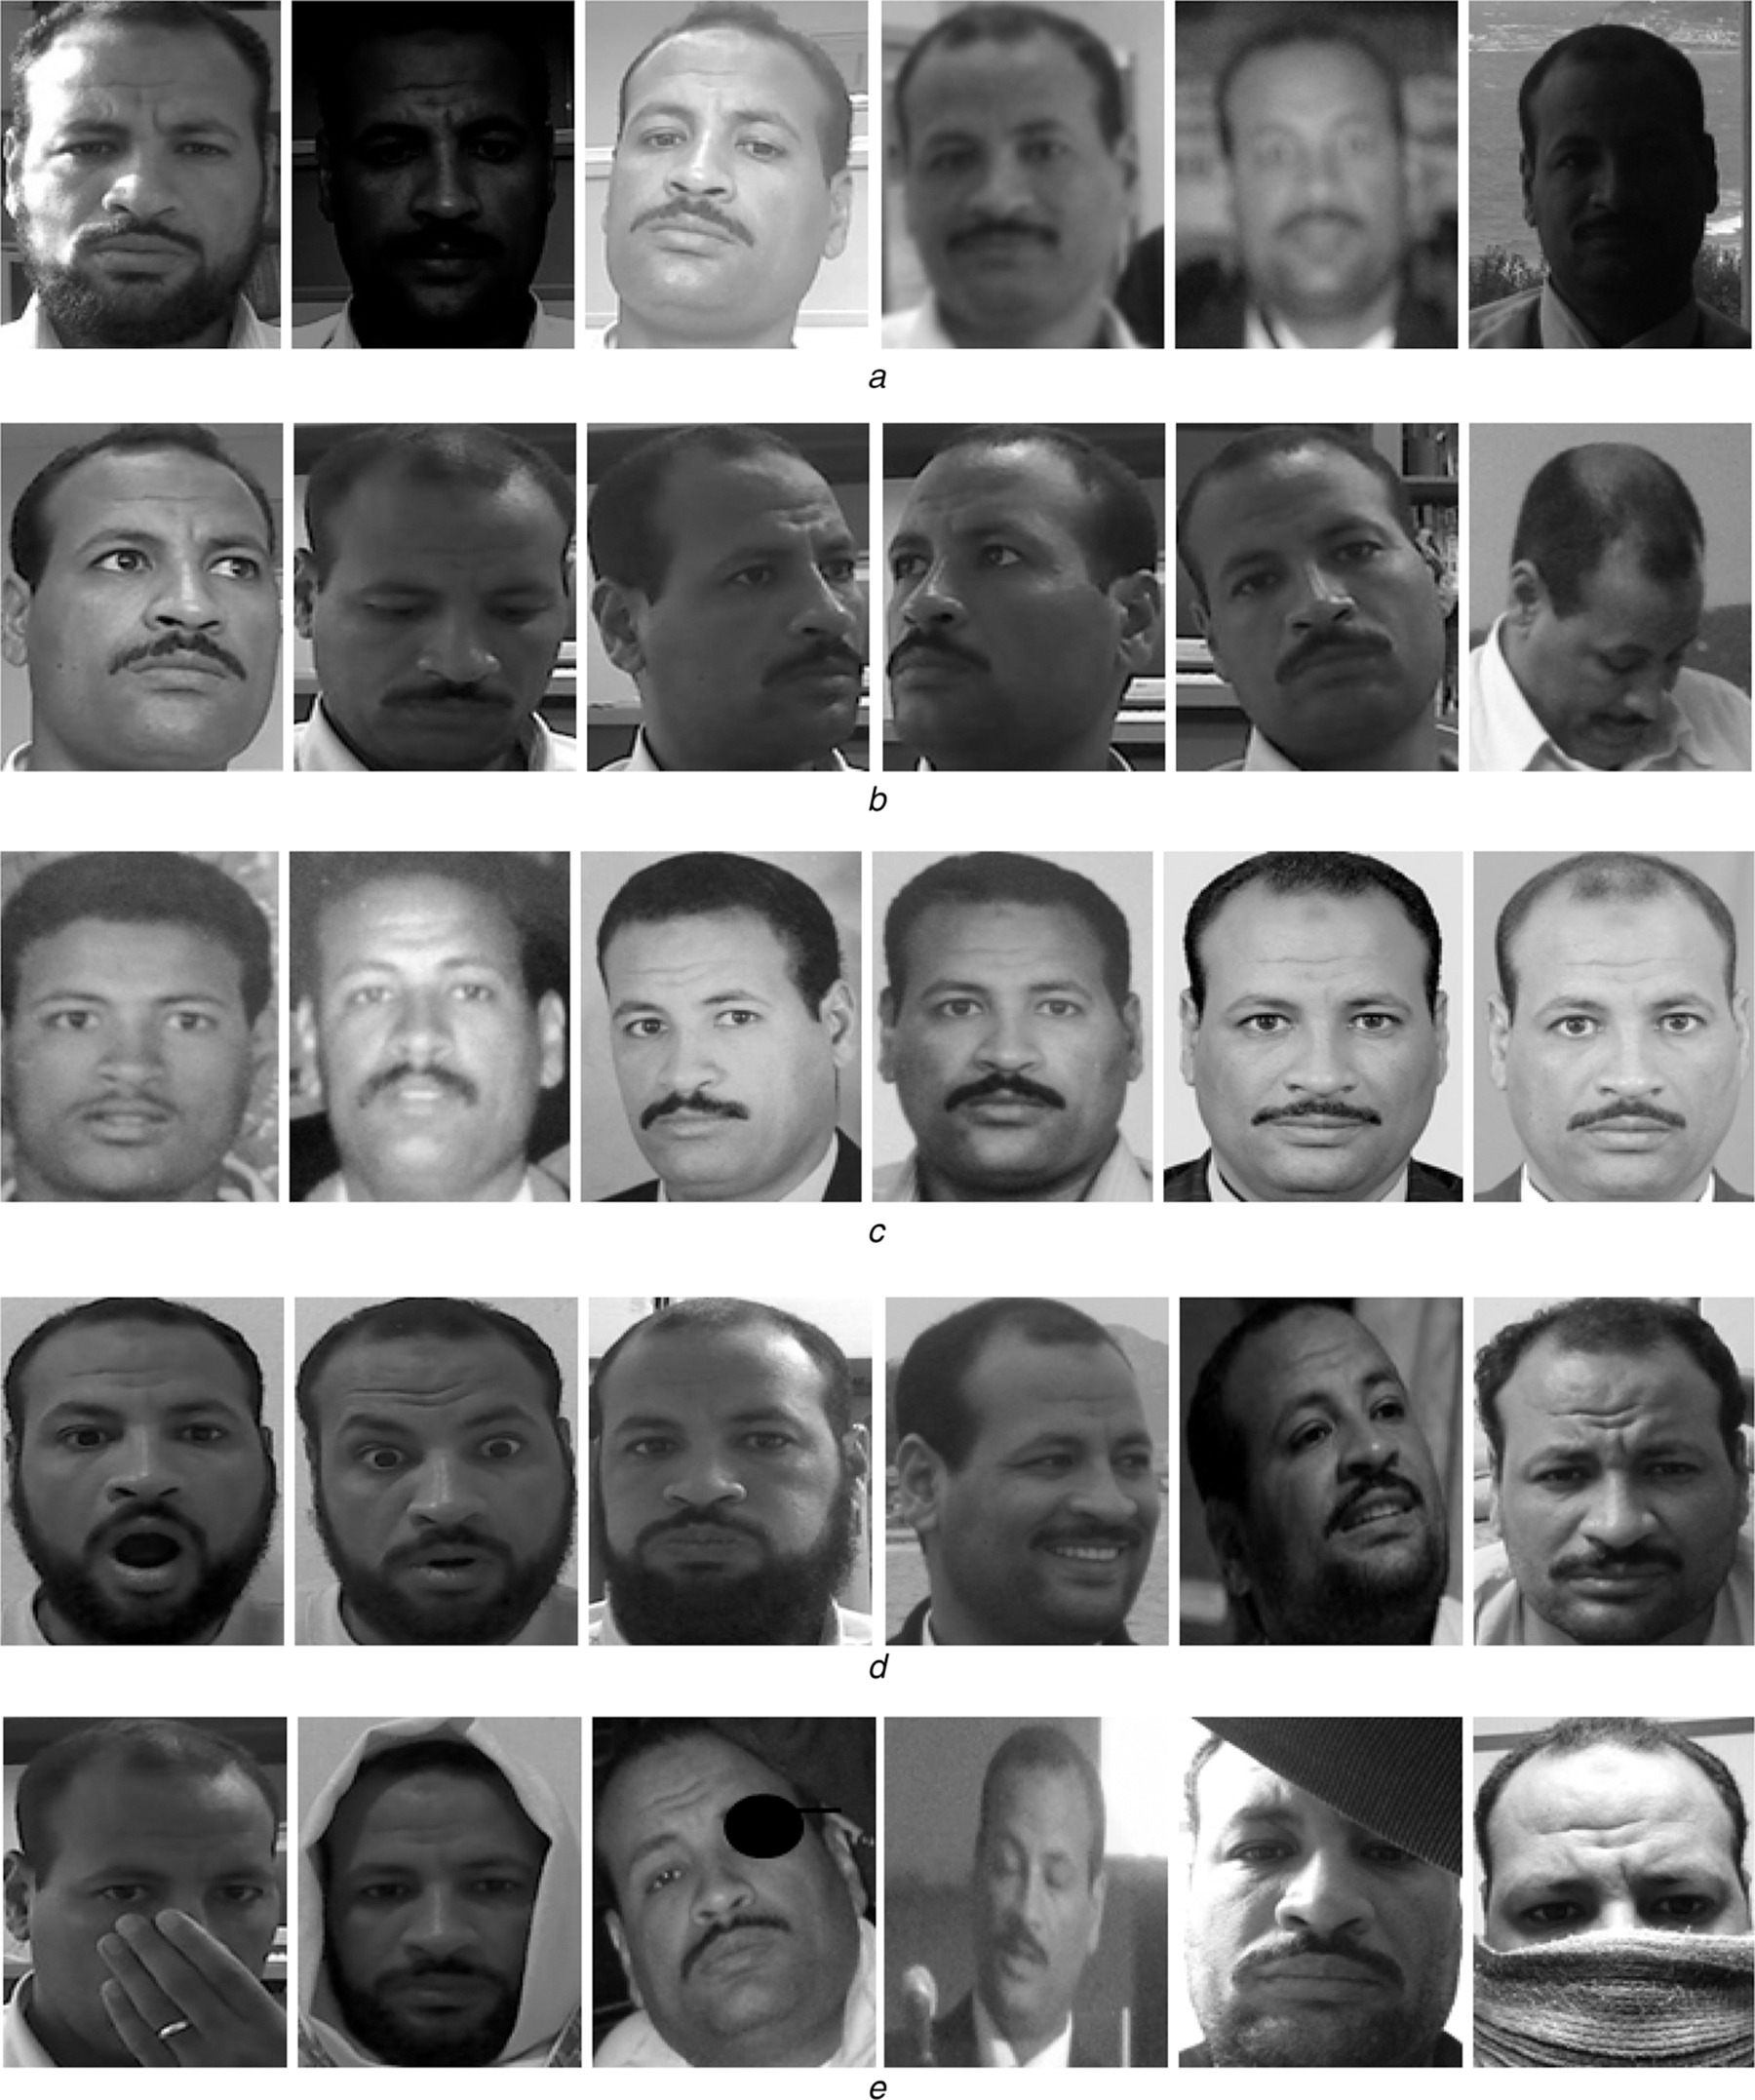
\includegraphics[width=\textwidth]{figures/facedetection_challenge.jpeg}
	\caption{Arcfelismerést nehezítő kihívások szemléltetése \cite{9}}
	\label{fig:face2}
\end{figure}

\newpage

\subsection{Megvilágítási variációk}
A kép kialakítása során olyan tényezők, mint a megvilágítás (spektrumok, forráseloszlás és intenzitás) és a kamera jellemzői (érzékelő reakciója és lencsék) bizonyos mértékig befolyásolják az emberi arc megjelenését.
Egy robusztus és hatékony arcfelismerő rendszer kivitelezése során a megvilágítás problémáját tekintik a rendszertervezők előtt álló egyik fő műszaki kihívásnak, ahol az ember arca eltérőnek tűnhet a fényviszonyok tekintetében \cite{11}.
A megvilágítás variációira vonatkozó jelenlegi megközelítések többsége erős feltételezéseket tesz, amelyeket a gyakorlatban nagyon nehéz teljesíteni.
A fényviszonyok vagy a pózok változásainak kezelésére a póz-robusztus albedóbecslésen alapuló képújravilágítási technika használható ugyanazon személy több frontális képének előállítására változó megvilágítás mellett \cite{12}. Az albedóbecslés egyik korlátja az, hogy a képek egymáshoz igazítását, valamint az arckifejezésekre való érzékenységet igénylik.


\subsection{Póz/nézőpont}

Az arcképek a kamera viszonylagos arcpózától függően változnak (elülső, 45°-os, profil, fejjel lefelé), és egyes arcvonások, például a szemek vagy az orr részben vagy teljesen eltakaródhat. Valójában a pózváltozások hatással vannak a felismerési folyamatra. Így a póztolerancia még kritikusabbá válik azoknál az arcfelismerő rendszereknél, amelyek az alany egyetlen nézetén alapulnak \cite{13}.


Blanz és munkatársai \cite{14} a nézőpontos arcfelismerési módszereket két alternatív paradigmába sorolta:  

\begin{itemize}
    \item Nézőpont-transzformált: előfeldolgozási módon működnek, és a becsült pózparaméterek alapján átalakítják a próbaképet, hogy azok illeszkedjen a galériában lévő képhez.
    \item Együttható alapú: megkísérli egyetlen kép alapján megbecsülni az arc fényterét; ez megtörténik a galéria és a próbaképek esetében is.
\end{itemize}

A póz problémájának megoldását 2D és 3D adatok kombinációjával is vizsgálják.


\subsection{Öregedés és ráncok}

Az öregedés lehet természetes (az életkor előrehaladása miatt) és mesterséges (sminkeszközök használata).
Az öregedés és a ráncok mindkét esetben súlyosan befolyásolhatják az arcfelismerő rendszerek teljesítményét. Általánosságban elmondható, hogy az arcfelismerési kutatások során általában nem veszik figyelembe az életkor változásának hatását. Az egyik fő oka annak, hogy az arcfelismeréssel kapcsolatos, életkori tényezővel összefüggésben megvalósuló tanulmányok kis száma miatt nem állnak rendelkezésre reprezentatív nyilvános adatbázisok, amelyek különböző életkorú egyéneket tartalmazó képeket tartalmaznának, valamint közrejátszik a régi képek alacsony minősége is, amint azt a szakirodalom dokumentálja.\cite{15}. Nagyon nehéz olyan arcképekhez olyan adathalmazt gyűjteni, amely ugyanarról a személyről, élete során, különböző életkorban készült képeket tartalmazna.


\subsection{Arckifejezés/arcstílus}

Az arcok megjelenését közvetlenül befolyásolja a személy arckifejezés. Az arcszőrzet, például a szakáll és a bajusz megváltoztathatja az arc megjelenését és az arc alsó felében, különösen a száj és az áll környékén. Ezenkívül a frizura megváltoztatható az arckép megjelenésének megváltoztatása vagy az arcvonások elrejtése érdekében. Aleix \cite{16} úgy fogalmazza meg az arcfelismerés problémáját az arckifejezés alatt, hogy „hogyan lehet robusztusan azonosítani egy olyan személy arcát, akinél a tanuló és a tesztelő arcképek arckifejezésében különböznek?”


\subsection{Eltakarás}

Az arcokat más tárgyak részben eltakarhatják. Egy embercsoportot ábrázoló képen egyes arcok vagy más tárgyak részben elfedhetnek más arcokat, ami viszont azt eredményezi, hogy sok helyzetben az arcnak csak egy kis része lesz látható. Ez azonban nehéz feladattá teszi az arcfelismerést a rendszer helye alapján, és még ha az arcot megtalálják is, maga a felismerés nehézségekbe ütközhet az arc egyes rejtett részei miatt, ami megnehezíti a felismerést \cite{17}.


\section{A személyazonosság-hitelesítési módszer, amely ötvözi az életszerűség-érzékelést (liveness) és az arcfelismerést}

A nagy sebességű processzorok és a nagy felbontású kamerák megjelenése a kutatás élére állt az arcfelismerő rendszerek különféle alkalmazásokhoz történő tervezésére. Az arcfelismerő rendszerek az alkalmazástól függően offline adatokat vagy valós idejű bevitelt használnak.


A \cite{18} tanulmányban egy fejlett Kinect érzékelőt alkalmaztak az életszerűség észleléséhez. Az infravörös sugárzás (IR) felvételeken alapuló életszerűség-észlelési módszer képes kezelni az archamisításokat. A jellemzők kinyerését és osztályozását egy mély neurális háló hajtotta végre, hogy különbséget tegyen a valódi személyek és az archamisítások között. A Kinect kamera által gyűjtött infravörös képek mélységi információkat tartalmaznak. Ezért az élő képek infravörös képpontjainak nyilvánvaló hierarchikus szerkezete van, míg a fényképek vagy videók képpontjainak nincs nyilvánvaló hierarchikus jellemzője. Ennek megfelelően kétféle IR-képet tanultak meg a mélyhálón keresztül annak megállapítására, hogy a képek élő egyedektől származnak-e. Más életszerűség-detektáló keresztadatbázisokkal összehasonlítva felismerési pontosságunk 99,8 százalék volt, és jobb, mint más algoritmusok. A FaceNet egy arcfelismerő modell, amely robusztus az elmosódáshoz és a megvilágításhoz. A személyazonosság-hitelesítéshez kombinálták az életszerűség-érzékelést és a FaceNet modellt. A kísérleti eredmények azt mutatták, hogy a javasolt életszerűség-érzékelés és a továbbfejlesztett arcfelismerés kombinációja jó felismerő hatással bír, és felhasználható személyazonosság-azonosításra.

Az arcfelismerés pontossága nagymértékben javul a mély tanulási hálók használatával, mivel képes kiemelni az emberi arcok mély vonásait.

Bár a továbbfejlesztett FaceNet keretrendszer más felismerő rendszerekhez hasonlóan pontosan képes felismerni az emberi arcokat, nem tudja megakadályozni a csalást. A legtöbb létező arcfelismerő rendszer sebezhető a hamisító támadásokkal szemben. Hamisító támadásról akkor beszélünk, ha valaki megkísérli megkerülni az arc biometrikus rendszerét, hamis arcot mutatva a kamera előtt.

A \cite{18} cikk olyan életszerűség-érzékelési megközelítést javasol, amely a Kinect kamerával nyert infravörös sugárzás (IR) képeken alapul. Az élő arcok infravörös képei pozitív mintaként jelennek meg, míg a fényképek vagy videók infravörös képei negatív mintaként. A fenti minták bemenetre kerülnek a konvolúciós neurális hálóba (CNN), hogy megtanulják az élő arcokat és a hamis támadásokat. Az életszerűség észlelése után a továbbfejlesztett FaceNet továbbra is felismeri az arcokat, és biztosítja a megfelelő azonosítót vagy az UNKNOWN kimenetet a pontos azonosítás érdekében.

Az arcfelismerés fokozatosan fontos titkosítási és visszafejtési módszerré vált gyorsasága, hatékonysága és felhasználóbarát jellege miatt. Az arcfelismerő technológia biztonsági kérdései azonban egyre hangsúlyosabbak. Ezért az életszerűség-érzékelés a megbízható hitelesítési rendszerek fontos részévé vált.

A gyakori hamisított arcok közé tartoznak a fényképek (nyomtatott), a videók (visszajátszás), a maszkok és a szintetikus 3D arcmodellek. Köztük a fotók és videók 2D hamis arcok, amelyek olcsóbbak a hamis támadásokhoz, és a megtévesztés két legnépszerűbb formája. Ezért az arcfelismerés gyakorlatiasságának és biztonságának javítása érdekében be kell vezetni az életszerűség-érzékelést a személyazonosság-hitelesítési rendszerekbe. 

Az elterjedt életszerűség-érzékelési módszerek főként textúrán, életinformációkon, különböző érzékelőkön és mély jellemzőkön alapulnak. Az élő arcok összetett 3D-s szerkezetekkel rendelkeznek, míg a fotó- és videótámadások 2D-s síkstruktúrák. A 3D és 2D struktúrák felületeinek különböző fényvisszaverődései különbségeket mutatnak az arcszínek világos és sötét területein. A textúra alapú módszerek főként ezeket a különbségeket használják támpontként az élő és a hamis arcok osztályozására. A textúrán alapuló detektálási módszert Local Binary Pattern (LBP) \cite{19} és továbbfejlesztett LBP \cite{20} algoritmusok segítségével valósítják meg. Ez a módszer alacsony számítási bonyolultságú és könnyen megvalósítható, de a hardverkörülmények nagymértékben befolyásolják. Az algoritmus pontossága csökken, ha a képminőség alacsony.

Az életjellemzőkre épülő módszer olyan életjeleket használ, mint a szívverés, a véráramlás, a pislogás és az arcizmok akaratlan mikromozgása az élő és a hamis arcok osztályozására. A kényszerfeltételek mellett ez a módszer nagy észlelési pontossággal rendelkezik, ha az életjellemzők stabilan kinyerhetők; ez a módszer azonban arcvideót igényel bemenetként, és nagy mennyiségű számítást igényel.

A különböző szenzorokon alapuló módszer különböző képgyűjtő rendszereket alkalmaz, például multispektrális kamerát, infravörös kamerát, mélykamerát, hogy megfelelő típusú emberi arcképeket rögzítsen az életszerűség érzékeléséhez. Ennek a módszernek az általános felismerési pontossága magas, de ehhez a módszerhez új hardvert kell hozzáadni, és így megnő a rendszer költsége. A mély jellemzőkre épülő módszerek magukban foglalják a kezdeti CNN tanítását a mélységi jellemzők kinyerésére, majd az osztályozást. Az arcfelismerő rendszerek fokozatos elterjedésével és a hardverek drágulásával szükséges és érdemes néhány fontos architelesítési rendszerbe képrögzítő berendezéseket beépíteni, azok biztonságának és megbízhatóságának javítása érdekében. Az arcok életszerűség-érzékelését valós mélységinformáció segítségével nem használják általánosan a biometrikus technológiában és a szakirodalomban.


\subsection{Módszertan}

Az infravörös képeket egy Kinect kamera rögzítette tanulóadatokként. A valódi arcokról származó adatok pozitív mintaként, míg a fotók vagy videók negatív mintaként szolgáltak arra, hogy a CNN-hálót megtanítsák annak megállapítására, hogy egy arc élő-e. Ezen túlmenően, mivel a FaceNet modell nagy arcfelismerési pontossággal rendelkezik, a továbbfejlesztett FaceNet élénkség-érzékelő algoritmussal kombinálva integrált hitelesítési rendszert alkot.

Az ~\ref{fig:face3} ábrán látható a javasolt keretrendszer, amely a FaceNet-et az élénkségérzékeléssel kombinálja, ahol CNN, konvolúciós neurális háló;  IR, infravörös sugárzás; MTCNN, többfeladatos kaszkádos CNN.


\begin{figure}[htbp]
	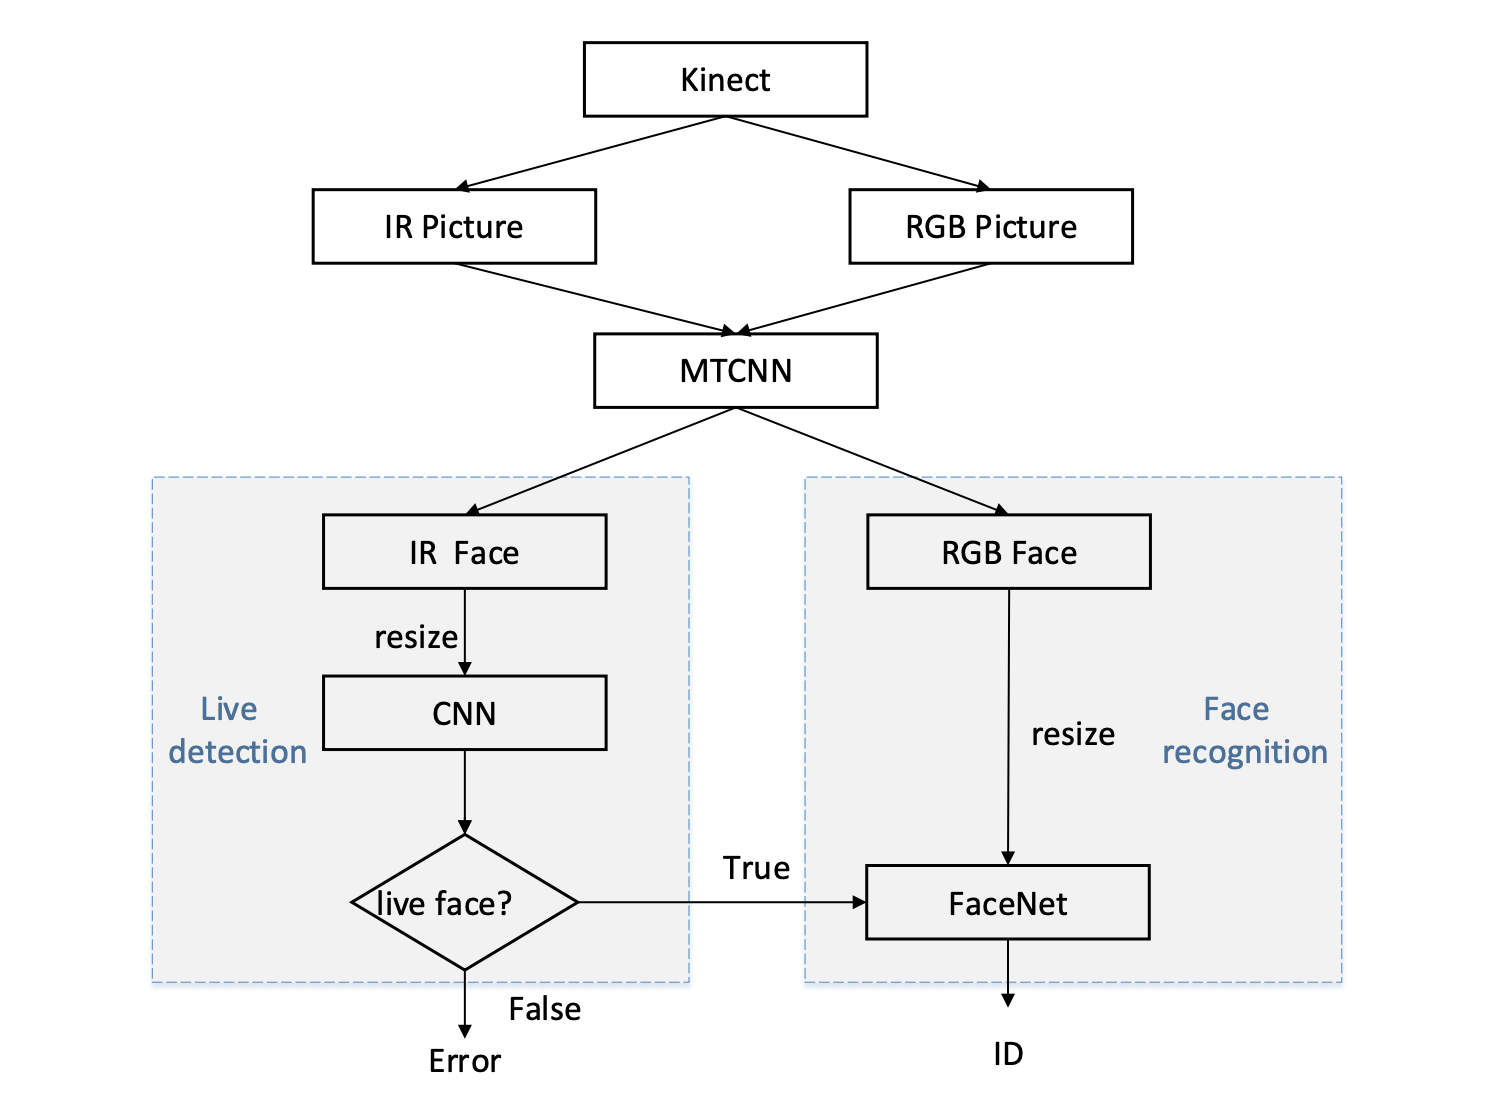
\includegraphics[width=\textwidth]{figures/live_rec.png}
	\caption{Életszerűség-érzékelésen és FaceNeten alapuló identitás-hitelesítési keretrendszer \cite{18}}
	\label{fig:face3}
\end{figure}

Először egy Microsoft Kinect kamerát használtak, amellyel RGB és IR képeket gyűjtöttek az emberi arcokról. Másodszor, egy multitask kaszkád konvolúciós hálót (MTCNN) használtak az RGB és IR képek arcrészeinek vágására és igazítására. Végül az MTCNN által feldolgozott infravörös képeket a CNN életszerűség-érzékelésére, míg az RGB képeket a FaceNet modell arcfelismerésre való betanítására használták. Ha az életszerűség-érzékelés eredményei igazak, az arcfelismerés folytatódik a teljes hitelesítési folyamat befejezéséhez. Ha az életszerűség-érzékelés hamis, akkor az algoritmus működése leáll, és az arcfelismerés többé nem történik meg.

\subsection{Életszerűség-érzékelés IR képjellemzők alapján}

Az IR képeken alapuló archamisítás-felismerés kétosztályos problémaként kezelhető. Ez a módszer a hamis arcok és a valódi arcok megkülönböztetésére szolgál. A javasolt életszerűség-érzékelési algoritmus a 3D arctér becslésére összpontosított. Kinect kamerát használtak a mély és szürke információkat tartalmazó infravörös képek készítéséhez. Ezeket a képeket bevitték a CNN-be, hogy megtanítsák az arcbőr textúrájára vonatkozó információkat. Mivel a teljes arctextúrákat figyelembe vették, a 2D-s megtévesztéseknek, például a fényképeket és videókat használóknak, már nincs hatása. Pozitív mintaként valós arcokról és bekeretezett valós arcokról készült IR-felvételek, negatív mintaként fotók, emberi arcokra ragasztott fotók és elektronikus eszközökön lévő fotók készültek, amiket aztán a CNN kapott meg, ahogy azt a ~\ref{fig:face3} ábra szemlélteti.

\begin{figure}[htbp]
	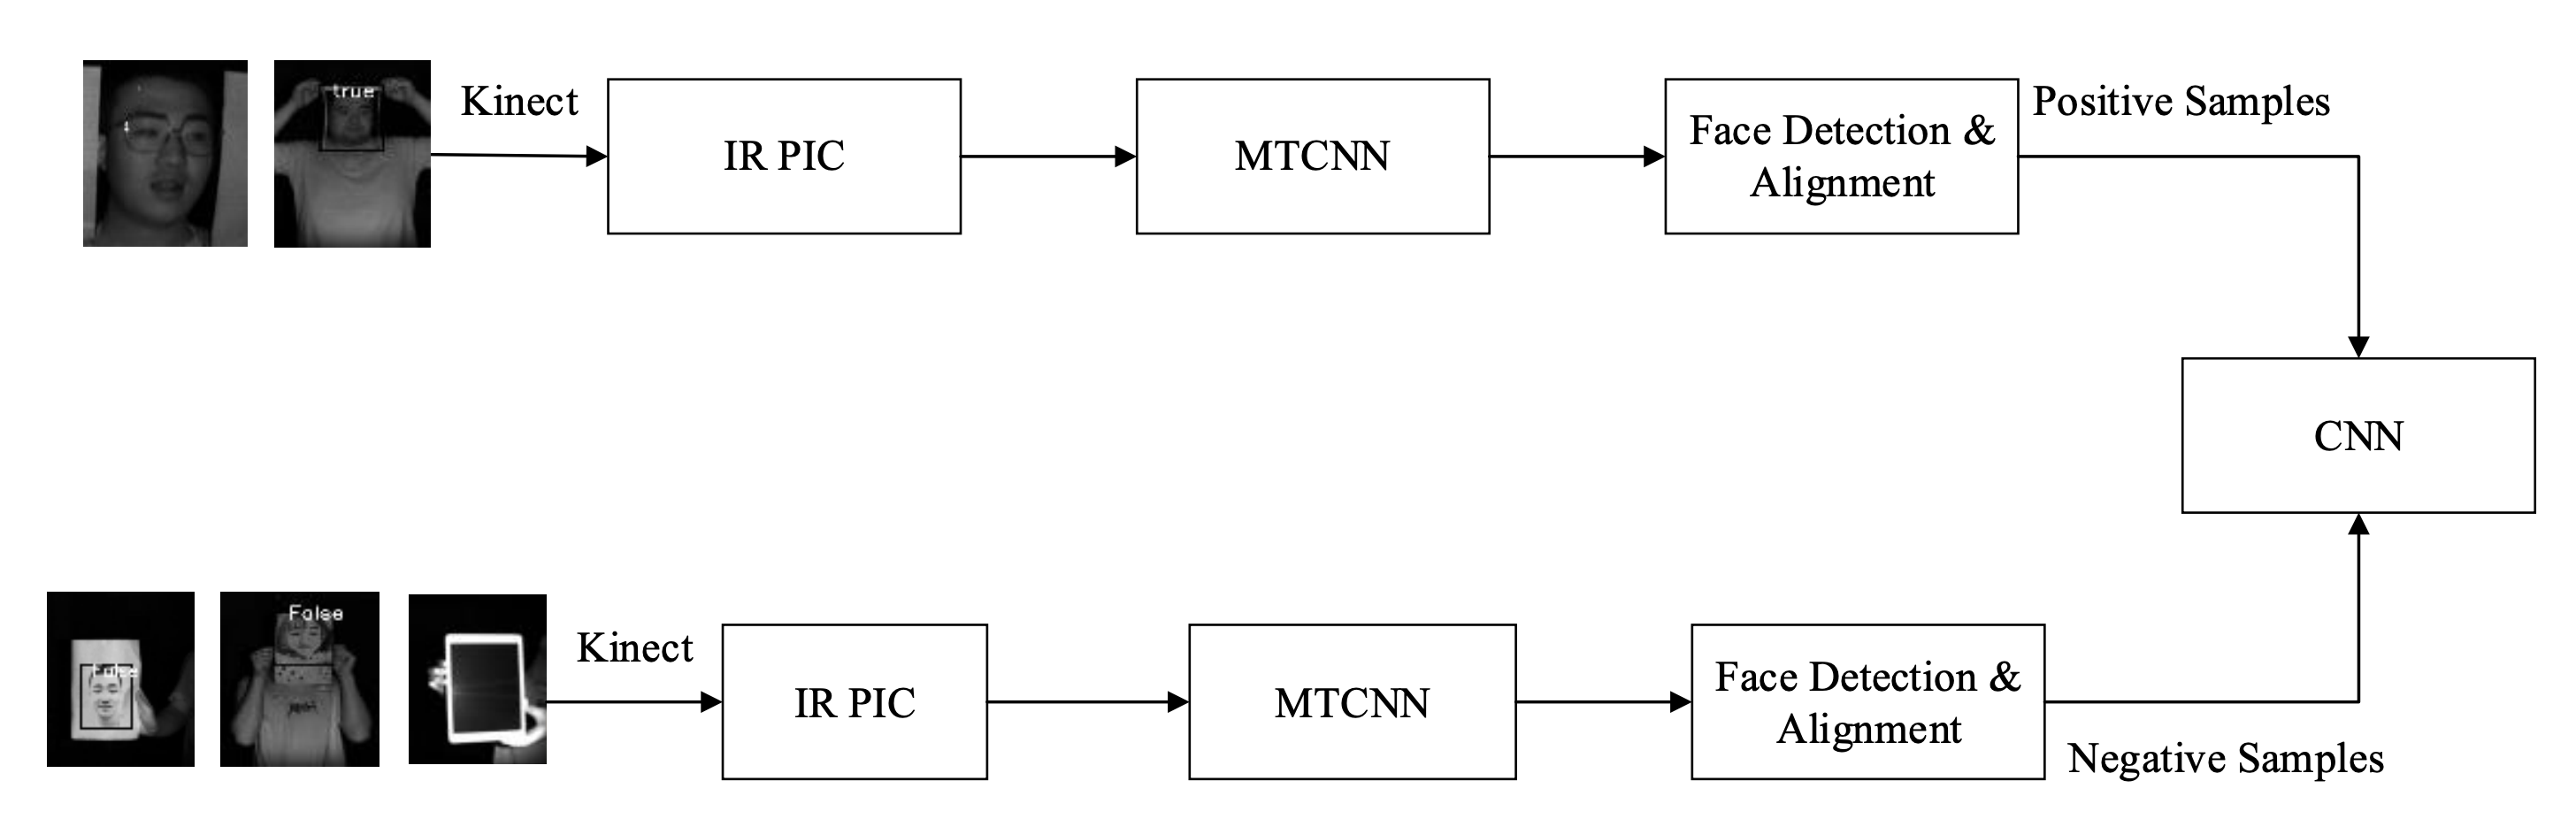
\includegraphics[width=\textwidth]{figures/live_training.png}
	\caption{Életszerűség-érzékelés tanulási folyamata \cite{18}}
	\label{fig:face4}
\end{figure}

\subsection{Összegzés}

Az olvasott tanulmány egy személyazonosság-hitelesítési rendszert javasolt, amely egy továbbfejlesztett FaceNet-modellt és egy életszerűség-észlelési módszert kombinál. A Kinect kamera által gyűjtött infravörös képek mélységi információkat tartalmaznak. Ezért az élő képek infravörös képpontjainak nyilvánvaló hierarchikus felépítése van, míg a fényképek vagy videók képpontjai nem rendelkeznek ezzel a funkcióval. A rendszer hatékonyan képes észlelni a 2D megtévesztést. Az élő arcok infravörös képi jellemzői nagymértékben eltérnek a fényképek vagy videókétól, így az életszerűség-észlelés bináris osztályozási problémaként kezelhető. Így a CNN-t úgy tervezték, hogy pontos életszerűség-felismerést valósítson meg. Az algoritmus nagy időhatékonyságú volt, és valós időben is alkalmazható.

\newpage

\section{Arcfelismerő modellek: melyiket használjuk és miért?}

A következőkben a \cite{21} cikk alapján olyan előre betanított modelleket vizsgálunk, mint a Haar-kaszkádok, a dlib frontális arcdetektor, az MTCNN (Multi-task Cascaded Convolutional Neural Network) és az OpenCV DNN-modulját használó Caffe modell, hogy megtudjuk, melyik működik a legjobban a valós idejű alkalmazások esetén, ezáltal melyiket érdemes használnunk a projekt kivitelezése során.

\subsection{Haar-kaszkádok (Haar Cascades)}

Gyors a munkavégzés, és az egyszerű CNN-hez hasonlóan sok jellemző kinyerésére képes a képekből. A legjobb jellemzőket ezután az Adaboost segítségével választja ki. Ez az eredeti 160 000+ jellemzőt 6000-re csökkenti, viszont mindezen jellemzők csúszóablakban történő alkalmazása még mindig sok időt vesz igénybe. Így bevezették az osztályozók kaszkádját, ahol a jellemzők csoportosítva vannak. Ha egy ablak meghibásodik az első szakaszban, akkor a kaszkád többi szolgáltatása nem kerül feldolgozásra. Ha megfelel, akkor a következő szolgáltatást tesztelik, és ugyanazt az eljárást megismétlik. Ha egy ablak képes átadni az összes jellemzőt, akkor az arcterületnek minősül.


A Haar-kaszkádok tanításához sok pozitív és negatív tanulókép szükséges. Szerencsére ezek a kaszkádok az OpenCV-könyvtárral és a betanított XML-fájlokkal együtt érkeznek.


\subsection{Dlib frontális arcérzékelő (Dlib Frontal Face Detector)}

A Dlib egy C++ eszközkészlet, amely gépi tanulási algoritmusokat tartalmaz valós problémák megoldására. Bár C++-ban van írva, különböző interfészeken keresztül lehetőségünk van Pythonban is használni. Ezenkívül rendelkezik a mérföldkőnek számító kulcspontérzékeléssel is.
A kulcspont-észlelés a kulcsobjektum-részek megtalálásából áll. Arcunk kulcsfontosságú részei például az orr, a szemöldökök, a szemzugok stb. A kulcspontérzékelés egyik fő alkalmazási területe az arcfelismerés.

A dlib által biztosított elülső arcdetektor az Orientált Gradiens Histogram (HOG) segítségével kinyert jellemzőket használ, amelyeket aztán egy SVM-en (Support Vector Machine) továbbítanak. A HOG jellemzőleíróban a színátmenetek irányainak eloszlását használjuk jellemzőként.


\subsection{Többfeladatos kaszkádos konvolúciós neurális hálózat (Multi-task Cascaded Convolutional Neural Network)}

Nem csak az arcot érzékeli, hanem öt kulcspontot is. Kaszkád struktúrát használ a CNN három szakaszával. Miután megvannak a jelöltek, ezeket átadják egy másik CNN-nek, amely visszautasítja a nagyszámú hamis pozitív eredményt, és elvégzi a határolókeretek kalibrálását. Az utolsó szakaszban az arc kulcspontjainak észlelését hajtják végre.


\subsection{DNN arcérzékelő az OpenCV-ben (DNN Face Detector in OpenCV)}

Ez egy Caffe modell, amely az SSD-n (Single Shot-Multibox Detector) alapul, és a ResNet-10 architektúrát használja. Az OpenCV 3.3 után került bevezetésre a mély neurális hálózati moduljában.

\subsection{A képeken elért eredmények összehasonlítása}

A tanulmány során a modellek teszteléséhez két típusú képeket használtak: nagy méretű és felbontású Unsplash fotókat és kis méretű Google fotókat.
Az első esetben mivel a képek átlagos mérete 5000x5000 körül volt, a feldolgozás előtt a magasságot és a szélességet is felére kellett csökkenteni. Míg a Google képek esetén az átlagos képméret 220x220, feldolgozásuk az eredeti állapot szerint történt, kivéve a DNN-modult, ahol a képeket 300x300-ra méretezték át, mivel az eredmény nem volt jó, ha eredeti méretű képeket használtak.

Mindezek alapján alkalmazva a négy modellt, a következő eredmények születtek:

\begin{itemize}
    \item A Haar eléggé elavult, és általában a legrosszabb eredményeket adta.
    \item Az OpenCV DNN moduljának arcfelismerő modellje jól működött, de ha a kép mérete nagyon nagy, az problémákat okozhat. Általában nem dolgozunk ilyen 3000x3000-es képekkel, így ez ebben az esetben nem számít akkora problémának.
    \item A Dlib nem érzékeli a 80x80-nál kisebb arcokat, így ha kis képekkel dolgozunk, győződjünk meg arról, hogy felskáláztuk őket, de ez megnöveli a feldolgozási időt is.
    \item A fenti két szempontot figyelembe véve tehát az MTCNN lenne a legjobb megoldás, ha extrém arcméretekkel kellene megküzdenünk, és elmondható, hogy a mai napig vezeti a versenyt.
\end{itemize}

\subsection{A modellek összehasonlítása videók esetén}



A felvételek esetén a következő szempontok alapján tesztelték a modelleket:

\begin{itemize}
    \item Az arc különböző szögei
    \item Mozgó fej
    \item Az arc eltakarása
    \item Különböző fényviszonyok
    \item Elért képkockasebesség (fps)
\end{itemize}

A modelleknek átadott keretek mérete 640x360, és a feldolgozás az eredeti állapot szerint történt, kivéve a DNN modellt, amely esetén a méretet 300x300-ra csökkentették.

Mindezeket figyelembe véve az alábbi következtetéseket vonták le:

\begin{itemize}
    \item A Haar Cascade osztályozó a teszt többségében a legrosszabb eredményt adta, sok téves pozitív eredmény mellett.
    \item A Dlib és az MTCNN nagyon hasonló eredményeket ért el, enyhe előnyt szerzett az MTCNN, mivel a Dlib nem tudja azonosítani a nagyon kicsi arcokat. Abban az esetben, ha a képek mérete nagyon extrém, jó megvilágítás, minimális kitakarás mellett és főleg, ha az arcok elülső része van előtérben, akkor az MTCNN a legjobb eredményt nyújthatja, ahogyan azt a képek összehasonlításakor láthattuk.
    \item Általános számítógépes látási problémák esetén az OpenCV DNN-modul Caffe modellje a legjobb. Jól működik kitakarás esetén, gyors fejmozgással, és az oldalsó arcokat is képes azonosítani. Ráadásul a leggyorsabb fps-t is ez adta az összes közül.
\end{itemize}


\subsection{Következtetés}

A tanulmány keretein belül végzett vizsgálat során levont következtetéseket szem előtt tartva döntöttünk úgy, hogy az általunk alkalmazott életszerűség-érzékelő algoritmus modelljeként a OpenCV DNN-modul Caffe modellje lesz a legjobb választás. Figyelembe vettük, hogy egy valós idejű jelenlétkezelő rendszer esetében számunkra azok az eredmények a mérvadóak amelyek a videófelvételek vizsgálata során születtek. Mivel ebben az esetben a Caffe modell szerepelt legjobban, főleg a képkockasebesség tekintetében (12.95 fps), úgy döntöttünk, hogy ezt a megoldást fogjuk alkalmazni a rendszerünk hatékony működése érdekében.
    %----------------------------------------------------------------------------
\chapter{Szoftver követelmények} \label{chapter6}
%----------------------------------------------------------------------------

A különböző szoftver követelményeket tekintve a Tanár és Diák mobilalkalmazások egyetlen mozzanatban változtak: 

\begin{itemize}
    \item {Nem a Diák applikáció feladata a diákazonosító létrehozása.}
    \item {A diák azonosítása és a jelenlétek mentése az adatbázisba nem a Tanár applikáció feladata.}
\end{itemize}

\section{Felhasználói követelmények}

\subparagraph* {Arcfelismerő és életszerűség-érzékelő modul}\
\newline
\begin{itemize}
    \item {A diákok azonosításához szükséges képek mentése, Neptun azonosító, név és szak megadásával.}
    \item {Diákok azonosítása, az arc bekeretezésével és a név feltüntetésével, majd a jelenlét mentése.}
\end{itemize}

\subparagraph* {Diák alkalmazás}\
\newline
\begin{itemize}
    \item {Regisztráció és bejelentkezés, ami lehetővé teszi, hogy a diák bekerüljön a rendszerbe.}
	\item {Az órai jelenlétek utánkövetésének lehetősége, ami segít, hogy a diák bármikor megnézze saját jelenléteit és azok időpontját.}
	\item {Tanárnak való e-mail küldés.}
	\item {Belépés a Google tanterembe.}
	\item {Belépés a Neptun-ba.}\\
\end{itemize}

\subparagraph*{Tanár alkalmazás}
\begin{itemize}
	\item {Regisztráció és bejelentkezés, ami lehetővé teszi, hogy a tanár bekerüljön a rendszerbe.}
	\item {A jelenlétek megtekintése, keresési lehetőség név alapján.}
	\item {Részletes jelenlétek és azok időpontjának  megtekintése.}
	\item {Jelenlétek kimentése (letöltése), választható formátumban.}
	\item {Belépés a Google tanterembe.}
	\item {Csoportos e-mail küldése a diákoknak.}
	\item {Naptáresemény létrehozása és elküldése a diák számára.}\\
\end{itemize}

\subparagraph*{Adminisztrátor}

\begin{itemize}
	\item {Adatok karbantartása.}
	\item {Létrehozza a tantárgylistát, társítja a tanárokhoz a tantárgyakat, valamint létrehozza a Google tantermet minden tantárgyhoz.}\\
\end{itemize}


\section{Rendszer követelmények}
\subsection{Funkcionális követelmények}

\subparagraph*{Arcfelismerő és életszerűség-érzékelő modul}
\begin{itemize}
    \item Fényképek mentése: Kiválasztva a szakot, megadva a nevet és a Neptun azonosítót a diákról készül egy fénykép, ami mentésre kerül az előzőleg megadott adatok alapján elnevezve.
    \item Jelenlétek mentése: Kiválasztva a tárgyat, annak típusát, a szakot, az aktuális hetet és a termet, elindul a kamera, ami által azonosítva lesznek a diákok, azt követően jelenlétük mentésre kerül az adatbázisba.
\end{itemize}


\subparagraph*{Diák alkalmazás}
\begin{itemize}
    \item {Regisztráció és adatok validálása: szak kiválasztása legördülő listából, teljes név, pontosan 6 karakter hosszúságú Neptun azonosító, e-mail cím, amely eleget tesz a formátumnak, minimum 6 karakter hosszúságú jelszó, majd ezek tárolása NoSQL adatbázisban, a \enquote{Regisztráció} gomb lenyomásával.}

	\item {Bejelentkezés: a korábban regisztrált e-mail és jelszó párossal, a \enquote{Bejelentkezés} gomb lenyomásával.}
	
	\item{\enquote{Elfelejtetted a jelszavad? Kattints ide!} szövegre kattintva lehetséges új jelszó beállítása, amit a regisztrált e-mail címre küldött linkkel tehet meg.}
	
	\item {E-mail cím visszaigazolása a regisztrált e-mailcímre elküldött link alapján, illetve amennyiben nem érkezett meg az e-mail, a \enquote{Visszaigazoló e-mail újraküldése} gombbal megismételhető a procedúra.}
	
	\item {\enquote{Jelenlét megtekintése} gombra kattintva, kiválasztható a tantárgy és annak típusa legördülő listából.}
	
	\item{A \enquote{Megjelenítés} gombra kattintva, láthatóvá válik a meglévő jelenlétek száma, és a részletes jelenléti adat egy listában: a hét és a beviteli dátum.}
	
	\item {\enquote{Egyéb alkalmazások} lehetőséget választva a diák három lehetséges opcióból választhat: \enquote{E-mail küldése a tanárnak}, ami lehetővé teszi a tanárnak való üzenetküldést a tanár nevének kiválasztása alapján, az e-mail cím ismerete nélkül. \enquote{Belépés a Google tanterembe} és \enquote{Belépés a Neptunba} opciók az adott alkalmazások megnyitását biztosítják.}\\
\end{itemize}


\subparagraph*{Tanár alkalmazás}
\begin{itemize}
	\item {Regisztráció és adatok validálása: teljes név, pontosan 6 karakter hosszúságú Neptun azonosító, e-mail cím, amely eleget tesz a formátumnak, minimum 6 karakter hosszúságú jelszó, majd ezek tárolása NoSQL adatbázisban, a \enquote{Regisztráció} gomb lenyomásával.}
	
	\item {Bejelentkezés: a korábban regisztrált e-mail és jelszó párossal, a \enquote{Bejelentkezés} gomb lenyomásával.}
	
	\item{\enquote{Elfelejtetted a jelszavad? Kattints ide!} szövegre kattintva lehetséges új jelszó beállítása, amit a regisztrált e-mail címre küldött linkkel tehet meg.}
	
	\item {\enquote{Korábbi jelenlétek megtekintése}: szak, tantárgy és annak típusának kiválasztásával egy listából, a 
	\enquote{Diákok megjelenítése} gombra kattintva megjelenik a jelenléti lista a diákok neveivel, valamint egy keresősáv, amely lehetővé teszi a diákok neve alapján való keresést.}
	
	\item {Egy diákot kiválasztva további adatok megtekintésére van lehetőség a diák jelenléteivel kapcsolatban, amely által látható a diák neve, és jelenléti adatai egy listában: hét, dátum.}
	
	\item {\enquote{Jelenlétek exportálása} menüpont lehetővé teszi tantárgy és formátum függvényében való letöltést, ahol a kívánt tantárgyat egy legördülő listából választható, valamint annak formátuma is.}
	
	\item {\enquote{Belépés a Google tanterembe}: kiválasztva az adott tantárgyat, az alkalmazáson keresztül megnyitható a tanterem linkje.}
	
	\item {\enquote{Naptáresemény létrehozása} opció lehetővé teszi adott tantárggyal kapcsolatos esemény létrehozását, majd kiküldését a kiválasztott Google tanterem diákjainak.}
	
	\item {Az \enquote{E-mail küldése} lehetőség a csoportos e-mail küldést jelenti a diákok felé, szak és tantárgy függvényben.}\\
\end{itemize}


\subparagraph*{Adminisztrátor}
\begin{itemize}
	\item{Hozzáférés az adatbázisban tárolt adatokhoz.}
	\item{A tanár tantárgyainak kezelése: tantárgy hozzárendelése a tanárhoz az adatbázisban a már meglévő tantárgylistához.}
	\item{Google tanterem kezelése: minden tantárgyhoz létrehoz egy tantermet, és ennek URL címét szintén tárolja az adatbázisban lévő erre a célra létrehozott listában.}\\
\end{itemize}


\subsubsection{Nem-funkcionális követelmények}

\begin{itemize}
    \item {Az arcfelismerő és életszerűség-érzékelő modul futtatásához szükség van egy webkamerával felszerelt számítógépre vagy egy laptopra ami szintén rendelkezik webkamerával.}
    \item {A diákok fényképeinek lementéséhez szükséges az elérhető lokális tárhely.}
    \item {A jelenlétek bevitelét, tárolását, valamint lekérését Firebase adatbázis biztosítja, aminek eléréséhez internetkapcsolat szükségeltetik.}
	\item {Az alkalmazások futtatása Android operációs rendszert támogató eszközön lehetséges, mindkét alkalmazás esetében  minimum Android 4.1 Jelly Bean (16. API szint) szükséges.}
	\item {A diák és tanár regisztrált adatainak tárolása ugyanúgy a valós idejű adatbázisban történik.}
	\item{Az azonosítás szintén a Firebase nyújtotta funkcióval valósul meg.}
	\item {Az aktuális jelenlétek lekérdezéséhez, valamint a regisztráció során küldött e-mail visszaigazolásához szintén internetkapcsolat szükséges.}
	\item {A Google tanterembe való belépéshez az internetkapcsolat mellett egy aktív Google fiókra is szükség van.}
	\item{A jelenléti adatok xlsx, pdf vagy csv formátumban exportálhatóak, ez a Google Apps szkripten keresztül valósul meg.}
	\item{A fájlok letöltése után, amennyiben meg szeretnénk nyitni, szükség van a megjelenítést lehetővé tévő alkalmazásra, például Excel.}
	\item{Az e-mail küldési lehetőséghez aktív e-mail fiókra van szükség, illetve egy e-mail küldő alkalmazás meglétére az adott eszközön.}
	\item{A naptáresemény létrehozásához, valamint megtekintéséhez egy Naptár alkalmazás szükségeltetik, a kiküldött események megtekintéséhez kifejezetten a Google naptár alkalmazásra van szükség.}
\end{itemize}

    %----------------------------------------------------------------------------
\chapter{A rendszer részletes bemutatása} \label{chapter7}
%----------------------------------------------------------------------------

\section{Rendszer architektúra}

A rendszer architektúrája az alapfunkciót tekintve megváltozott. Minden \enquote{modul} egy közös Firebase adatbázisra csatlakozik, ahogy azt a ~\ref{fig:arch1} ábra is szemlélteti.

\begin{figure}[htbp]
	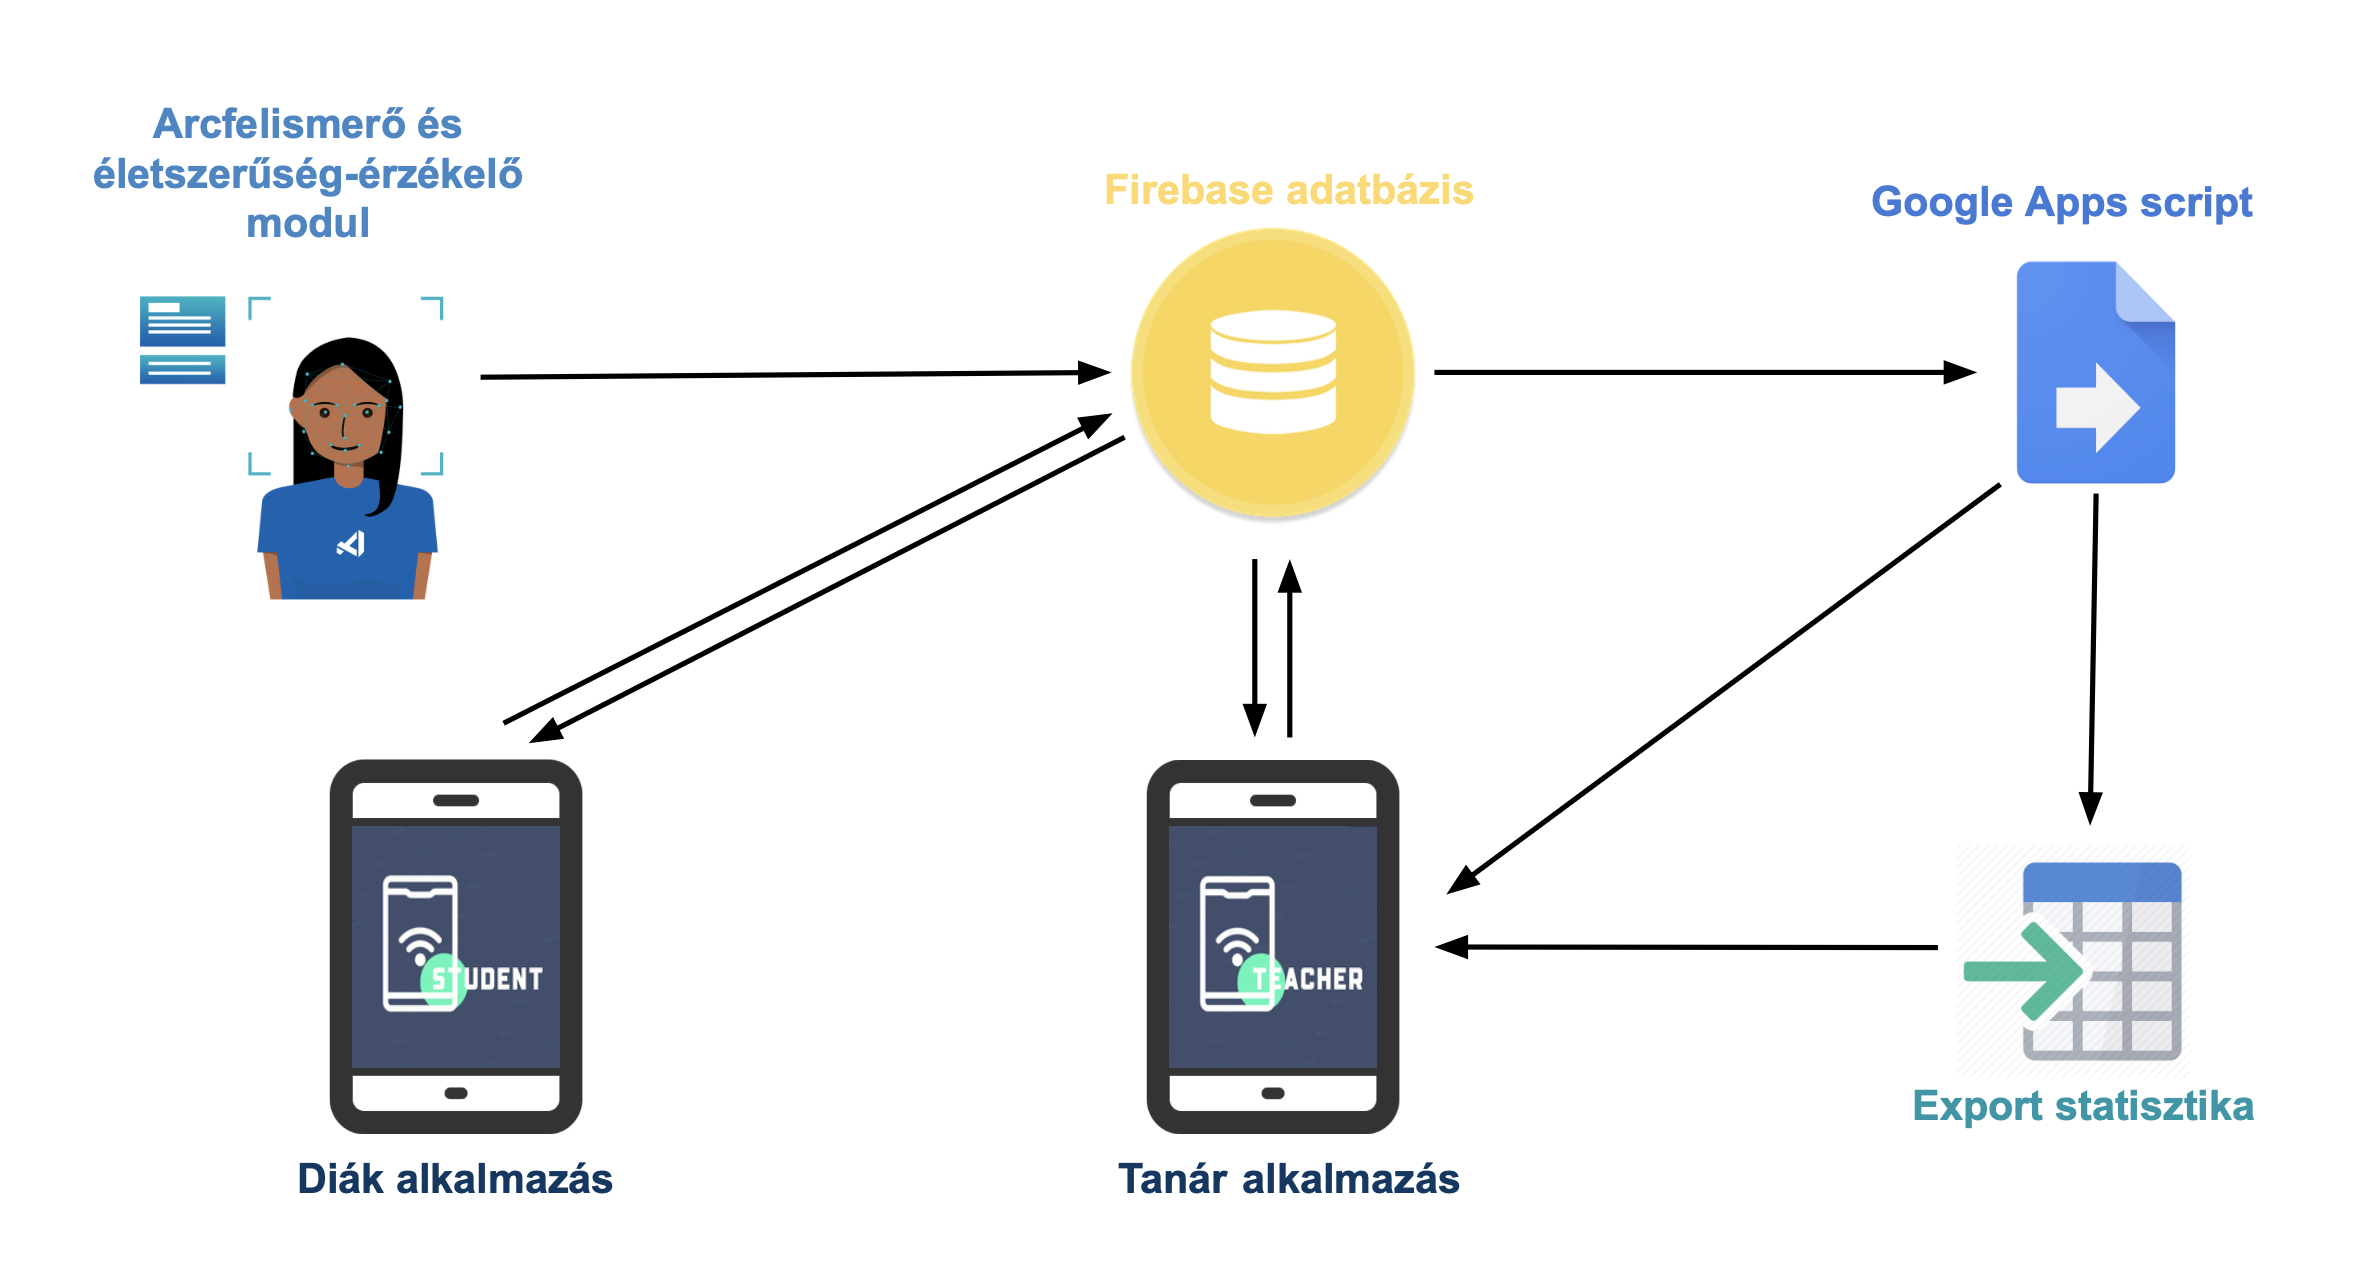
\includegraphics[width=\textwidth]{figures/architecture.png}
	\caption{A rendszer architektúrája}
	\label{fig:arch1}
\end{figure}

A rendszer a következő fő modulokból áll:

\begin{itemize}
    \item Arcfelismerő és életszerűség-érzékelő modul, amely felel a diákok azonosításáért, emellett szerepe a jelenlétek bevitele, valamint a diákok azonosításához szükséges előzőleges fényképek mentése is.
    \item Diák alkalmazás: fő feladata a jelenlétek megjelenítése a nyomon követhetőség elősegítése végett.
    \item Tanár alkalmazás: a jelenlétek megtekintése mellett fontos funkciója a jelenlétek kimentésének biztosítása különböző formátumokban.
    \item Google Apps script: ez teszi lehetővé a jelenlétek táblázatban való megjelenítését, amely az exporthoz szükségeltetik.
\end{itemize}


Amint az látható, architektúra szempontjából az arcfelismerő és életszerűség-érzékelő modulon kívül a rendszer többi része majdhogynem változatlan maradt, ennek okáért a továbbiakban csak az említett részt szeretném tárgyalni.


\paragraph{Arcfelismerő és életszerűség-érzékelő modul}\

Maga a jelenlétkezelő modul 3 kulcsfontosságú funkcióból áll:

\begin{itemize}
    \item Diákok fényképeinek mentése.
    \item Arcfelismerő funkció, ami a diák azonosításáért felel.
    \item Életszerűség-érzékelő algoritmus, amelynek az átjátszhatóság elleni védelemben van meghatározó szerepe.
\end{itemize}

\section{A diákok azonosítására használt fényképek mentése}

A hatékonyságot szem előtt tartva, a fényképek mentésére két megoldást próbáltunk ki.

Első megoldásként bővítettük a diákapplikáció funkcióit, méghozzá úgy, hogy a regisztrációkor az adatai mellett egy fotót is kell készítsen/feltöltsön magáról, amit a Firebase Storage-be mentettünk. Ezt a megközelítést bár lefejlesztettük, mégis eldobtuk két ok miatt. Egyrészt a diákot nem szeretnénk az applikáció használatára kényszeríteni. Ez azt jelenti, hogy csak akkor szükséges letöltenie, ha nyomon szeretné követni jelenléteit, illetve ha az app valamelyik másik funkcióját szeretné igénybe venni. Mivel a fénykép megléte kötelező jellegű, ezért láttuk jobbnak az alkalmazástól független megoldást keresni. A másik oka, miért nem ezt a megoldást választottuk az az, hogy nem szerettünk volna teljesen szabadkezet adni a fénykép milyensége végett a diáknak. Valamilyen szinten egységes fotókat szerettünk volna igényelni, éppen ezért döntöttünk úgy, hogy a fényképek készítése is az újonnan beépített modul feladata lesz. Ez azt jelenti, hogy a webkamera segítségével készül egy fotó a diákról, legelső órán, ezáltal mint minőségleg, mint pedig a \enquote{helyszínt} tekintve egységes képek fognak készülni.

A gyorsabb működés elérése érdekében egyelőre nem adatbázisba tároljuk a képeket, hanem lokálisan a jelenlétkezelő modult futtató gépen. Ez lehetővé teszi azt a megoldást is, hogy akár egy erre megbízott személy feltegye a diákok képeit tartalmazó mappát, amennyiben az egyetem rendelkezik vele.

\newpage

A fényképek mentésének kódbeli megvalósítását az alábbi kódrészlet szemlélteti:

\begin{lstlisting}[language=python]
if event == self.button_save:
    if values['class'] != "" and values['name'] != "" and values['neptun_id'] != "":
        cv2.imwrite('student-recognize-images/' + 
        values['neptun_id'] + "_" + 
        values['name'] + "_" + 
        values['class'] + '.png', frame)
        psg.popup('OK', 'Diak mentve!')
    else:
        psg.popup('Hiba', 'Minden mezo kitoltese kotelezo!')
\end{lstlisting}


\section{Diákok azonosítása: arcfelismerés}

Mivel előző megoldásunk, a QR kódos azonosítás, kijátszhatónak bizonyult, úgy döntöttünk, hogy a leggyakrabban alkalmazott biometrikus azonosítást, az arcfelismerést alkalmazzuk jelenlétkezelő rendszerünk alappilléreként.


A jelenlétek bevitelének elkezdését a mezők kitöltése után a kamera elindítása jelenti. Ezt követően megkapva az utolsó frame-et (\textit{get\_latest\_frame()}), két lista jön létre: az arcokat tartalmazó lista (\textit{face\_list}) és az életszerűség-érzékelés eredményét tartalmazó lista (\textit{live\_list}).

Ebben az alfejezetben az arcfelismerést fogom tárgyalni, melyet a \textit{face\_recognition\_process()} függvény biztosít. 

Az arcfelismerési procedúra lebonyolításához a Python \textit{Face Recognition} nevű könyvtárcsomagot használtuk. A dlib legmodernebb arcfelismerési funkciójával készült, mély tanulással.
A Dlib egy modern C++ eszközkészlet, amely gépi tanulási algoritmusokat és eszközöket tartalmaz komplex szoftverek létrehozásához C++ nyelven valós problémák megoldására. Az iparban és a tudományos életben egyaránt használják számos területen, beleértve a robotikát, a beágyazott eszközöket, a mobiltelefonokat és a nagy teljesítményű számítástechnikai környezeteket. A Dlib nyílt forráskódú licence lehetővé teszi, hogy bármilyen alkalmazásban ingyenesen használjuk.

A modell 99,38\%-os pontossággal rendelkezik a Labelled Faces in the Wild benchmarkon. A Labelled Faces in the Wild (LFW) arcfotók adatbázisa, amelyet a korlátlan arcfelismerés problémájának tanulmányozására terveztek.

A rendszer helyes működésének előfeltétele a diákok arcképeinek megléte. Ez az arcfelismerő modul működésének egyik kulcsfontosságú része, hiszen a meglévő képek szükségesek a megtalált arcok azonosításához.

Rendszerünk esetében, az elindítást követően szintén két listát hozunk létre: az első tartalmazza az arcok helyét (\textit{face\_locations(frame)}), azaz a talált arcok sorainak listáját téríti vissza (felső, jobb, alsó, bal) sorrendben. A második pedig az arcok kódolt értékét (\textit{face\_encodings(frame, face\_locations)}), ami alapvetően visszaadja s 128 dimenziós arckódolások listáját (a képen látható minden archoz egy). Ugyanarról a személyről készült két különböző képnek hasonló a kódolása, és két különböző embernek teljesen eltérő a kódolása.

Ezt követően végig iterálunk a listákon és egy összehasonlítást végzünk a kódolt arcok és a megtalált arc között, majd megnézzük, hogy mekkora az arcok közötti távolság, hogy egyezésnek tekintsük. A 0,6 tipikusan a legjobb teljesítmény (\textit{compare\_faces(known\_face\_encodings, face\_encoding, tolerance=0.6)}). A művelet során egy Igaz/Hamis listát kapunk, amely jelzi, hogy mely ismert arckódolások felelnek meg az ellenőrizendő arckódolásnak.

Mindezek után távolságot számítunk, \textit{face\_distance(known\_face\_encodings, face\_encoding)}, ahol adott arckódolások listája kerül összehasonlításra egy ismert arckódolással, és  minden összehasonlítandó arc esetén euklideszi távolságot kapunk.
A távolság megmutatja, mennyire hasonlóak az arcok. Ezután kiválasztásra kerül a legjobb értékű index, azaz ahol a távolság a legkisebb, ezt pedig az \textit{argmin(face\_distances)} függvény határozza meg, amely egy tengely mentén a minimális értékek indexeit adja vissza.

Az arcfelismerés megtörtént, társítjuk a megfelelő névvel, majd átadásra és megjelenítésre bocsájtjuk a feldolgozott információk adott részét.

Az arcfelismerő algoritmus során használt függvényt a \textit{face\_recognition} könyvtárcsomag biztosította.

A diákok azonosítására használt arcfelismerést lehetővétévő függvény kódrészlete itt látható: 

\begin{lstlisting}[language=python]
def face_recognition_process(self, image, scaling_factor=4):
        face_names, face_list = [], []

        image = cv2.resize(image, (0, 0), fx=1.0 /
                           scaling_factor, fy=1.0/scaling_factor)
        rgb_image = image[:, :, ::-1]

        face_locations = face_recognition.face_locations(rgb_image)
        face_encodings = face_recognition.face_encodings(rgb_image, face_locations)

        for face_encoding in face_encodings:
            matches = face_recognition.compare_faces(
                self.known_face_encodings, face_encoding, tolerance=0.6)
            face_distances = face_recognition.face_distance(
                self.known_face_encodings, face_encoding)
            best_match_index = np.argmin(face_distances)

            name = self.known_face_names[best_match_index] if matches[best_match_index] else "Unknown"
            face_names.append(name)

        for (top, right, bottom, left), name in zip(face_locations, face_names):
            top *= scaling_factor
            right *= scaling_factor
            bottom *= scaling_factor
            left *= scaling_factor

            face_list.append(FaceDetectionData(name, left, top, right, bottom))

        return face_list
\end{lstlisting}

\section{Biztonsági ellenőrzés: életszerűség-érzékelés}

Bizonyára az első gondolat a rendszer szemlélése során, hogy mi teszi biztonságosabbá az előző verzióval szemben, miért ne lehetne átverni azt egy másik eszközön megjelenített fotóval vagy viedóval. A válasz egyszerű: életszerűség-érzékelés. 
Annak érdekében, hogy az arcfelismerő rendszereket biztonságosabbá tegyük, képesnek kell lennünk a hamis/nem valódi arcok észlelésére – az ilyen algoritmusok esetén az életszerűség-érzékelés kifejezést használjuk.

Az életszerűség-detektor létrehozása érdekében egy mély neurális hálózatot tanítunk, amely képes megkülönböztetni a valódi és a hamis arcokat, és ezt a bináris osztályozók problémájaként kezelik ebben az esetben. Mivel a projekt során nem szerettünk volna ennek részletes hátterével foglalkozni, így egy előre betanított modellt használtunk a megvalósításhoz (\textit{liveness.model}).

Első lépésként betöltjük a meglévő arcdetektáló és életszerűség-érzékelő modellünket.
Mivel a Caffe (Convolutional Architecture for Fast Feature Embedding) használata mellett döntöttünk, a \textit{cv2.dnn.readNetFromCaffe} segítségével töltjük be a Caffe modelldefiníciós prototxt fájlját és az előre betanított modellünket a lemezről.

A Caffe egy mély tanulási keretrendszer, amely lehetővé teszi a felhasználók számára, hogy képosztályozási és képszegmentációs modelleket hozzanak létre. Kezdetben a felhasználók sima szöveges prototxt fájlként hozzák létre és mentik el a modelleiket. Miután a felhasználó betanította és finomítja modelljét a Caffe segítségével, a program elmenti a felhasználó által betanított modellt \textit{caffemodel} fájlként.

Ezt követően készítünk egy blob-ot a frame-ből, melynek mérete 300×300, hogy alkalmas legyen a Caffe arcdetektor használata esetén. Ezt átengedjük a hálón, hogy megkapjuk a detektálásokat és predikciókat.

Meghatározzuk a detektált arc koordinátáit, majd kivesszük az észlelt arc ROI-ját (Region Of Interest).

A predikció során megkapjuk a legnagyobb értéket, majd ezáltal meghatározunk egy score-t. Mivel nekünk is van egy előre megadott érték, ami fölött az arcot valódinak tekintjük, így összehasonlítást végezve megkapjuk a valós arcokat. Ellenben, ha ez a megkapott érték kisebb az általunk megadott küszöbértéknél, hamis arcnak tekintjük, amiket majd nem veszünk figyelembe a további műveletek végrehajtása során.

\newpage

Az életszerűség-észlelést az alábbi függvény írja le:

\begin{lstlisting}[language=python]
def live_detection_process(self, image):
        (h, w) = image.shape[:2]
        blob = cv2.dnn.blobFromImage(cv2.resize(image, (300, 300)),
                                     1.0,
                                     (300, 300),
                                     (104.0, 177.0, 123.0))

        self.net.setInput(blob)
        detections = self.net.forward()

        detection_list = []
        for i in range(0, detections.shape[2]):
            confidence = detections[0, 0, i, 2]

            if confidence > self.confidence:
                box = detections[0, 0, i, 3:7] * np.array([w, h, w, h])
                (startX, startY, endX, endY) = box.astype('int')

                startX = max(0, startX)
                startY = max(0, startY)
                endX = min(w, endX)
                endY = min(h, endY)

                face = image[startY:endY, startX:endX]
                face = cv2.resize(face, (32, 32))
                face = face.astype('float') / 255.0
                face = img_to_array(face)
                face = np.expand_dims(face, axis=0)
            
                predictions = self.model.predict(face)[0]
                max_index = np.argmax(predictions)
                score = predictions[max_index]

                if score > self.min_live_score and max_index == self.is_live:
                    detection_list.append(LiveDetectionData(
                        score, 'real', startX, startY, endX, endY))
                else:
                    detection_list.append(LiveDetectionData(
                        score, 'fake', startX, startY, endX, endY))
                        
        return detection_list
\end{lstlisting}

\newpage

\section{A jelenlét rögzítésének és a fénykép mentésének aktivitás diagramja}

Amint azt a ~\ref{fig:arch1} ábra (1) szemlélteti, a jelenétek bevitele az ábrázolt folyamat szerint megy végbe. A \textit{Kezdés} gomb megnyomásával elindul a detektálás. Amennyiben egy arc felismerésre kerül, azaz tudtuk azonosítani, az életszerűség-ellenőrzés veszi kezdetét. Ellenkező esetben nem történik azonosítás, csupán a felületen megjelenítjük az \textit{Unknown} címkét.

A következő lépésben az algoritmus el kell döntse, hogy élő arcot lát-e vagy sem. Amennyiben élő arcot érzékel, az azonosított diák jelenléte mentésre kerül az adatbázisba. Ellenkező esetben szintén nem történik semmilyen művelet, egy újabb címkével jelezzük, hogy az arc \enquote{hamis}.

A ~\ref{fig:arch1} ábra (2) mutatja be a fénykép mentésének folyamatát. Az alkalmazás indítása után, amennyiben az adott diák/diákok adatai még nem kerültek mentésre, az \textit{Új diák hozzáadása} lehetőséget választva ezt pótolni tudjuk. Ezt követően szükséges megadunk a kért adatokat, mint a szak, név és Neptun azonosító, és ezt követően tudjuk elkészíteni a fényképet, amit aztán lokálisan is lementünk.


\begin{figure}[htbp]
	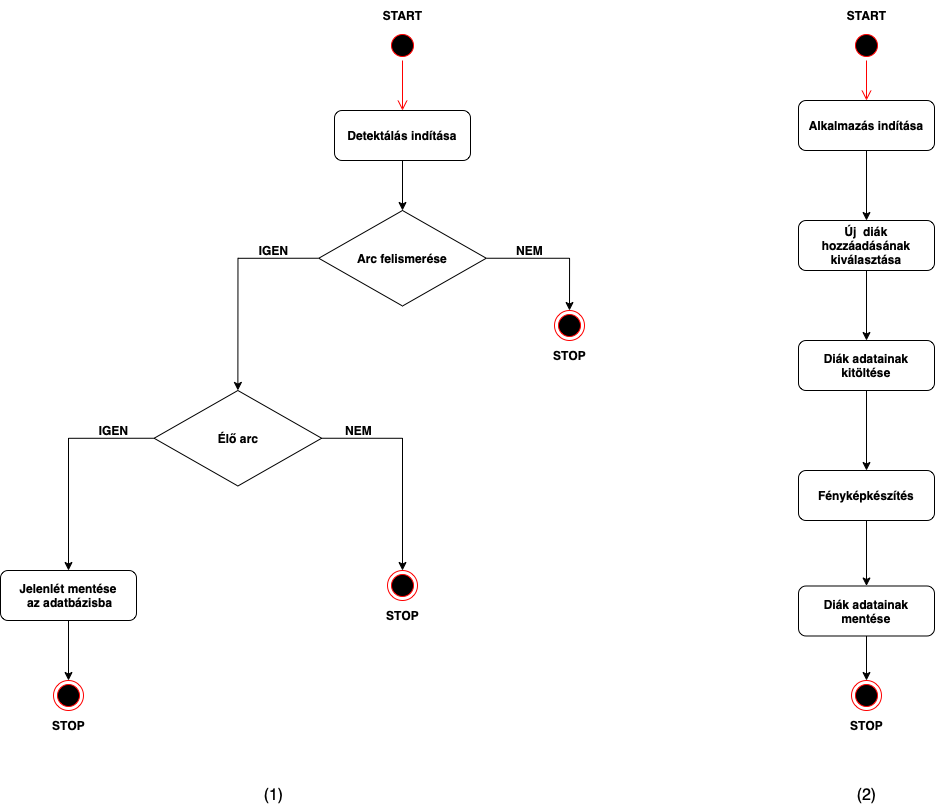
\includegraphics[width=15cm,height=12cm]{figures/activity11.png}
	\caption{A jelenlét rögzítésének (1) és a fénykép mentésének (2) aktivitás diagramja}
	\label{fig:activity1}
\end{figure}






    %----------------------------------------------------------------------------
\chapter{A rendszer gyakorlati működésének bemutatása} \label{chapter8}
%----------------------------------------------------------------------------

Az alábbiakban szeretném bemutatni az élő arcfelismerés-alapú jelenlétkezelő alkalmazás fő működési folyamatait, a mobilalkalmazásokkal együtt.

Ahhoz, hogy a diák jelenlétét tudja igazolni először is szükség van egy róla készült fotó mentésére, ami szintén a rendszer egyik funkciója. Ezzel a művelettel, kiválasztva a megfelelő szakot, megadva a nevet és Neptun azonosítót, egy kattintásra mentve lesz a kép az erre kijelölt mappába. Ezen mozzanat látható a ~\ref{fig:gy1} ábrán.

\begin{figure}
	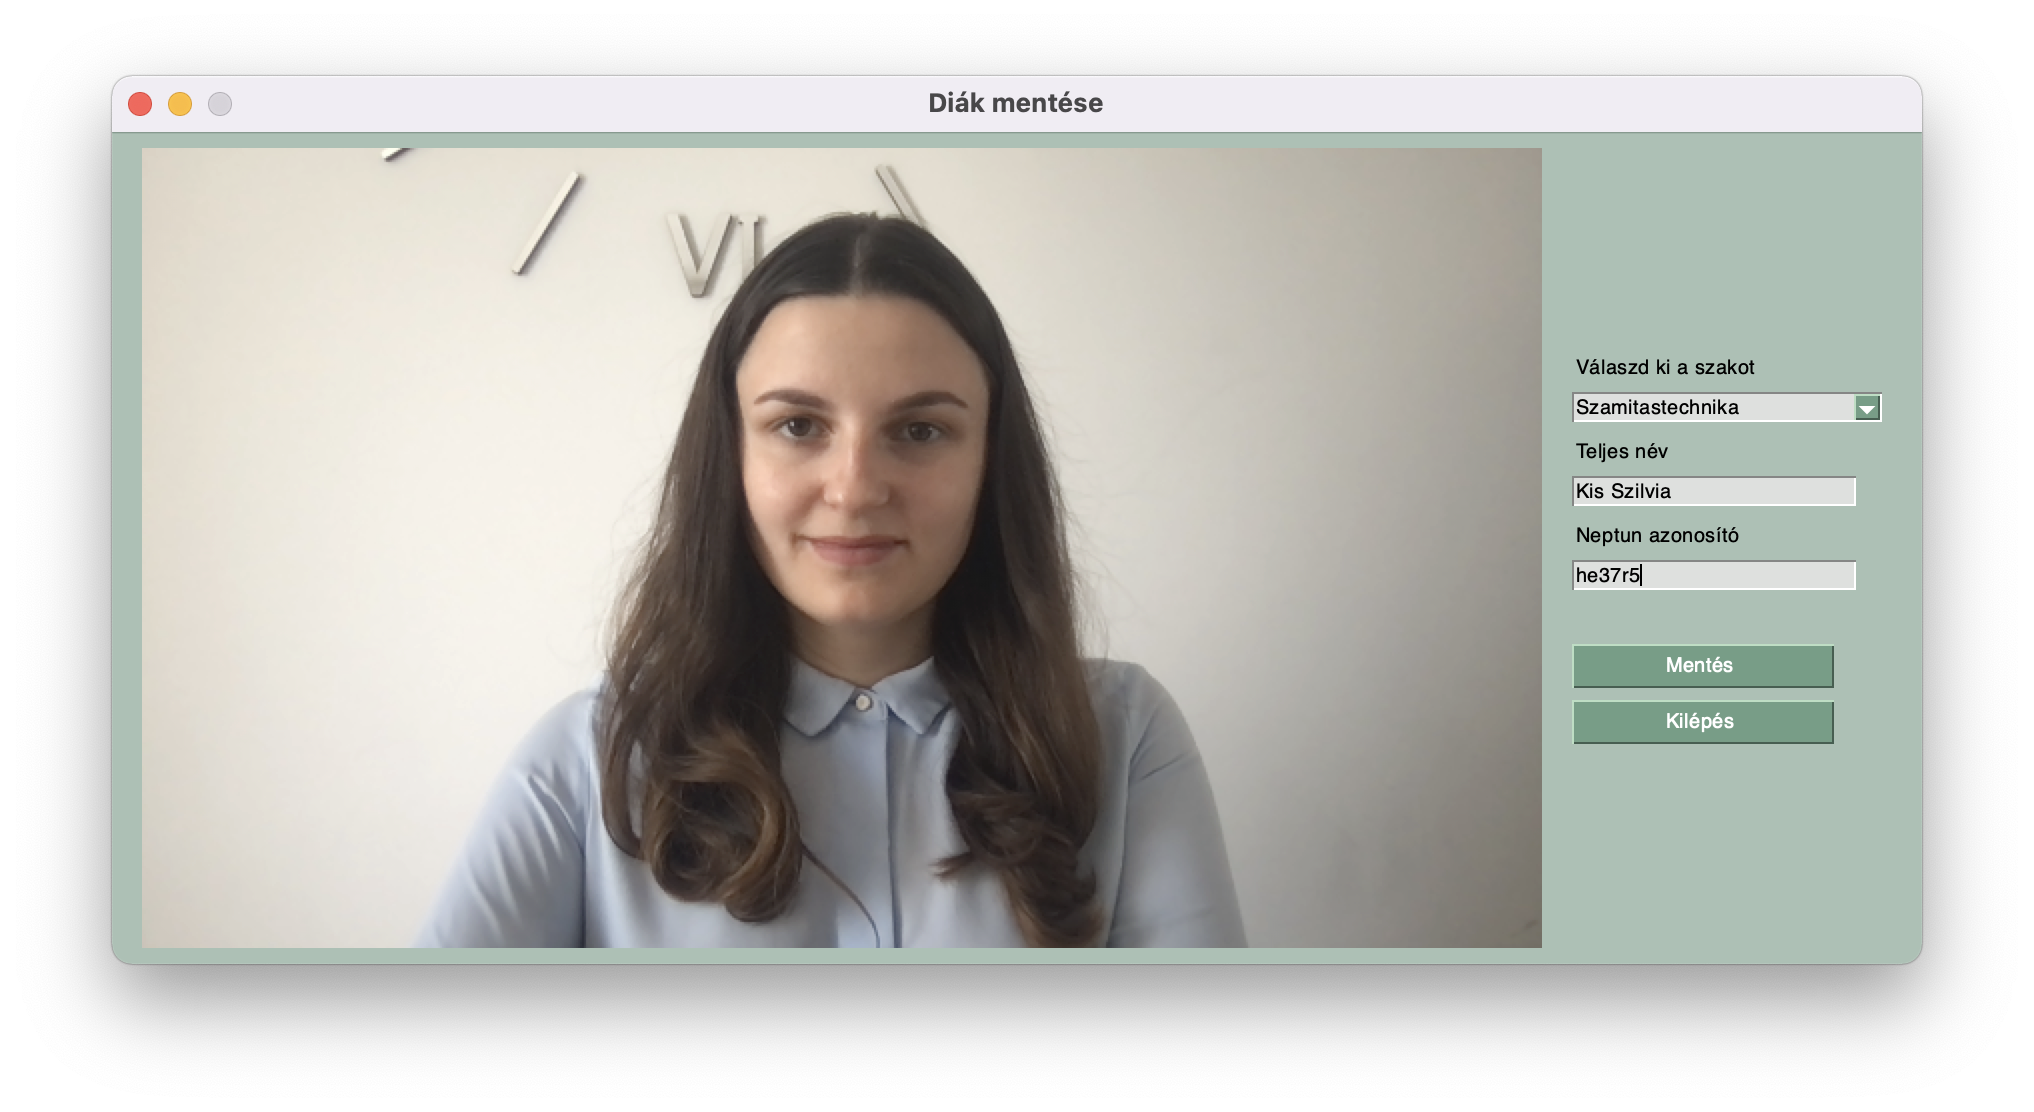
\includegraphics[width=\textwidth]{figures/gy1.png}
	\caption{Diák fényképének mentése}
	\label{fig:gy1}
\end{figure}


Miután minden hallgató bekerült a rendszerbe, indulhat a jelenlétek bevitele. Ehhez csupán annyit kell tenni, hogy a tanár beállítja az órai adatokat, majd a diákok elsétálnak a kamera előtt. Egyszerre akár több diák is azonosítható. A helyes azonosítás végett a képernyőn zöld keret jelenik meg, ahol a név és az életszerűség-érzékelés eredményét is feltüntetjük a könnyen értelmezhetőség kedvéért, ahogy azt a ~\ref{fig:gy2} ábra is mutatja.

\begin{figure}
	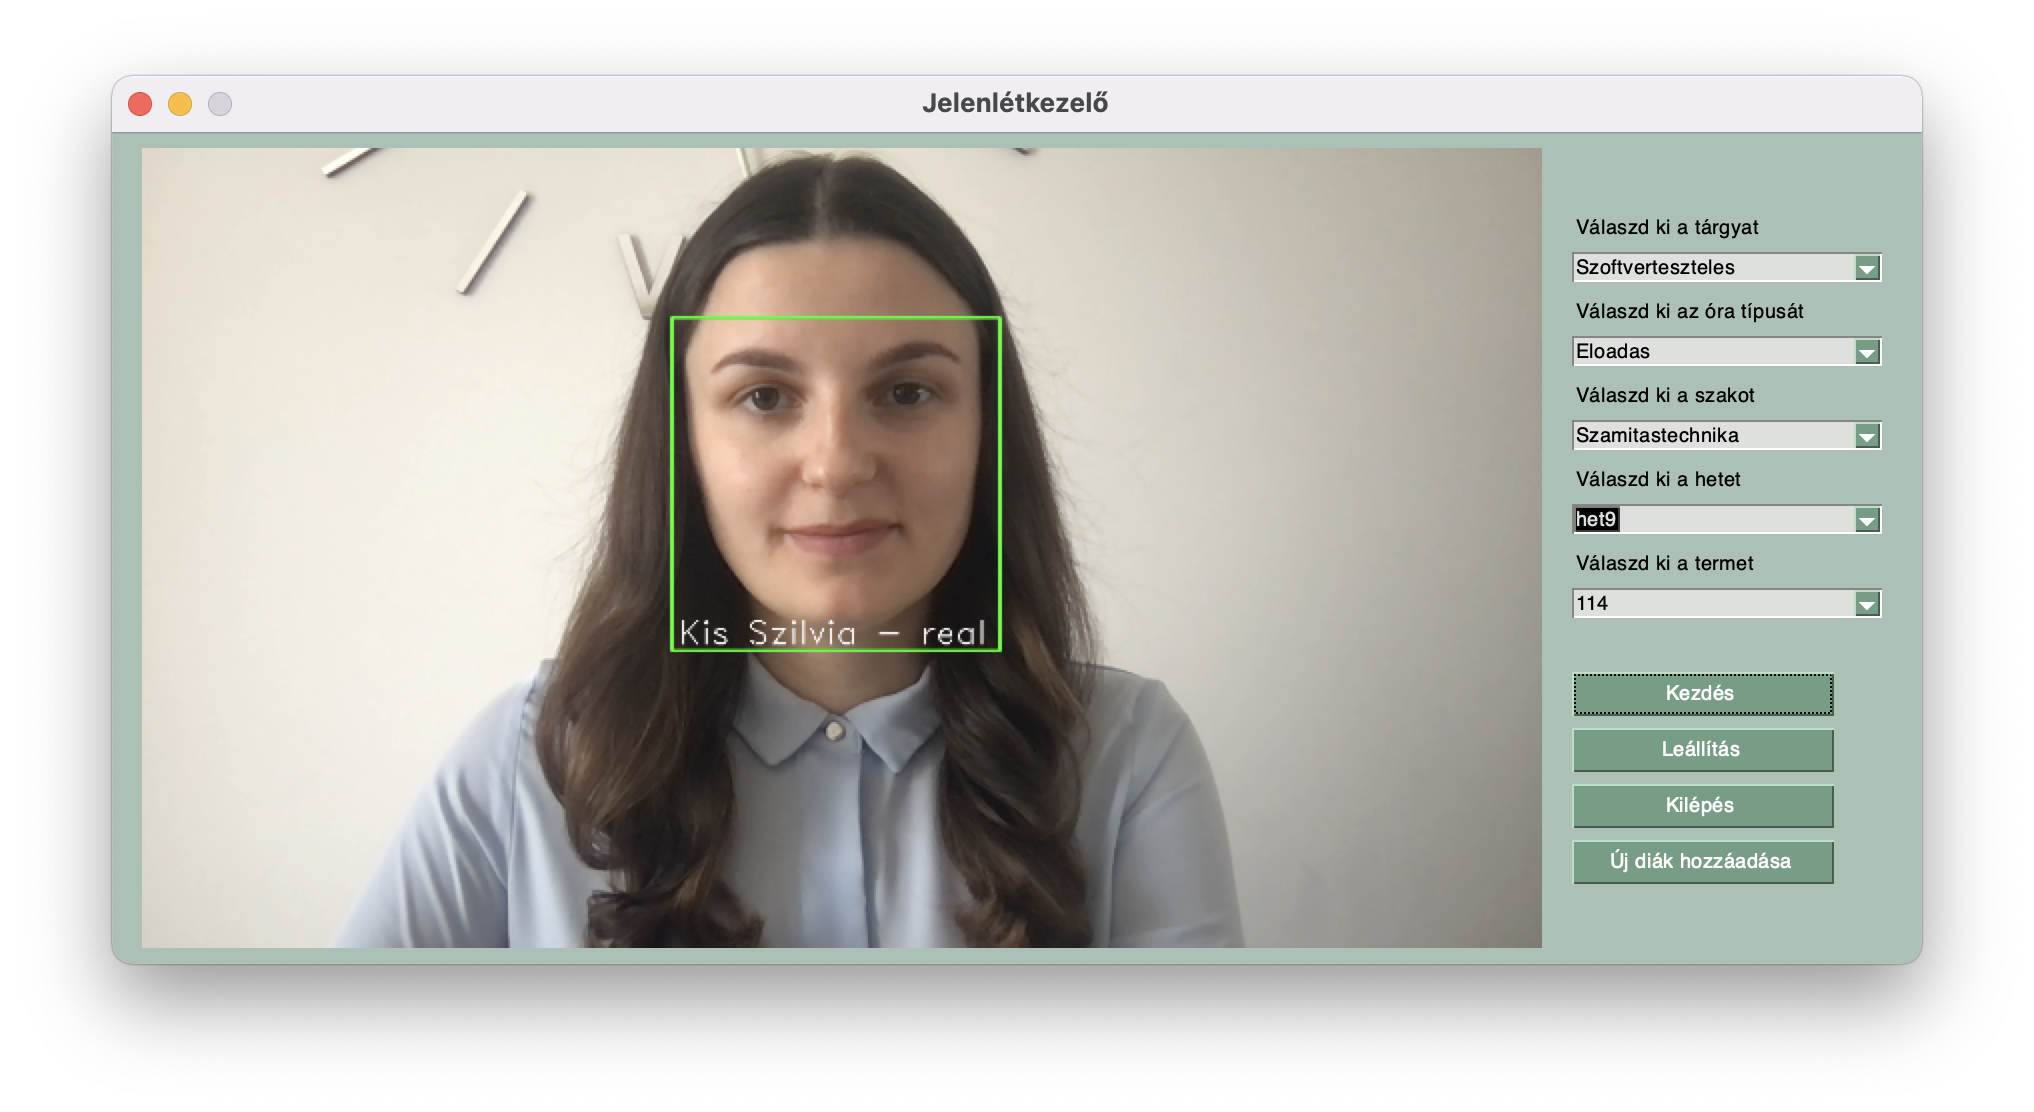
\includegraphics[width=\textwidth]{figures/gy2.png}
	\caption{Jelenlétek bevitele}
	\label{fig:gy2}
\end{figure}

Abban az esetben, ha egy olyan diák szeretné magát azonosítani, akinek adati nem ismertek a jelenlétkezelő alkalmazás részéről, egy \textit{Unknown} felirat jelenik meg, ami egy kattintással orvosolható: \textit{Új diák hozzáadása}. Ezt az esetet szemlélteti a ~\ref{fig:gy3} ábra.

\begin{figure}
	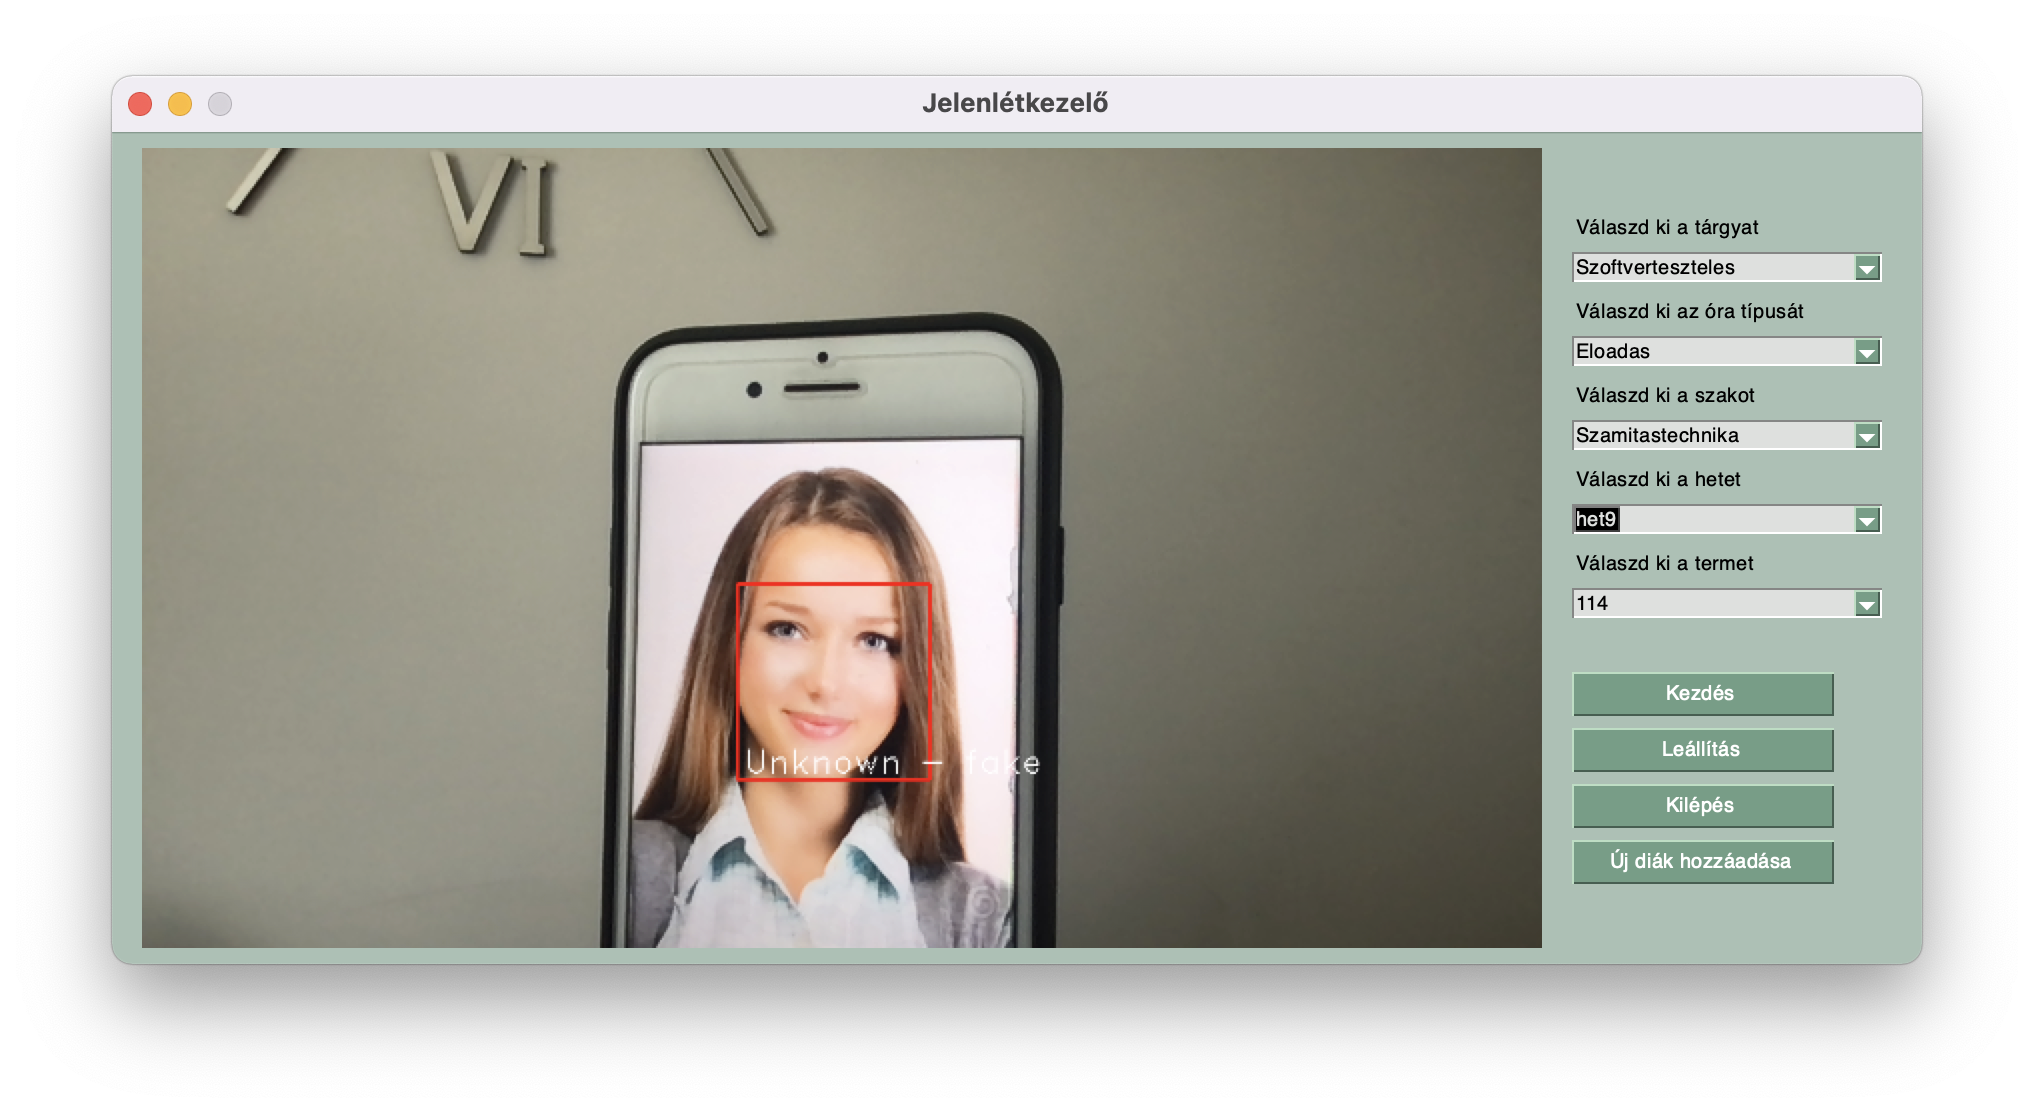
\includegraphics[width=\textwidth]{figures/gy3.png}
	\caption{Ismeretlen arc észlelése}
	\label{fig:gy3}
\end{figure}

A dolgozat fő kutatási témája az életszerűség-érzékelés, fő szerepet játszik a szoftver működésében, ugyanis ez az algoritmus felel a megbízhatóságért. Ez az jelenti, hogy a rendszert nem lehet olyan módszerekkel kijátszani, mint például egy másik diák fényképének mutatása akár fizikai fényképről vagy egy digitális eszközről. Abban az esetben ha a rendszer egy \enquote{hamis}, azaz nem élő arcot detektál, piros kerettel és a megfelelő felirattal jelzi ezt, amint az a ~\ref{fig:gy4} ábrán is látható.

\begin{figure}
	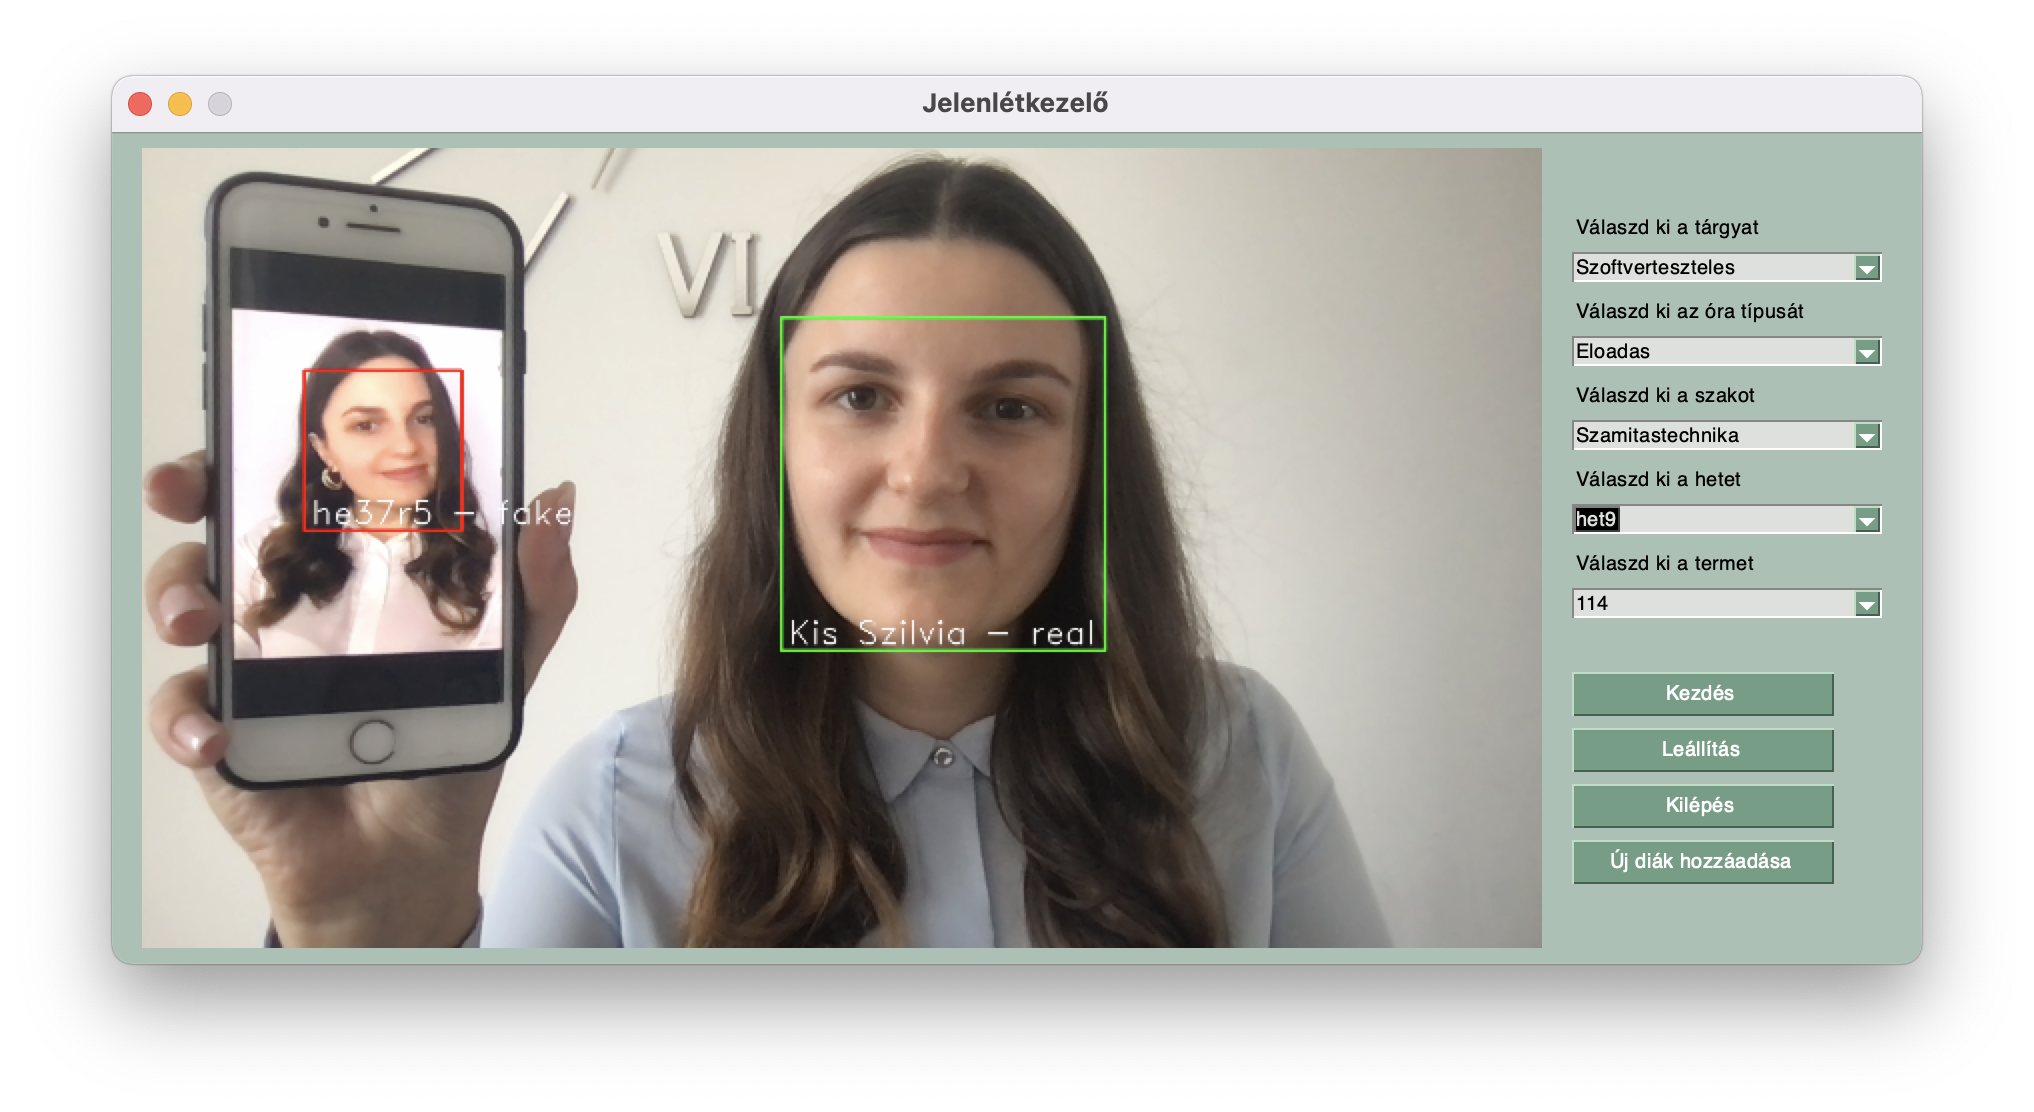
\includegraphics[width=\textwidth]{figures/gy4.png}
	\caption{Hamis és élő arc detektálása egyidejüleg}
	\label{fig:gy4}
\end{figure}

\newpage


Ezt követően minden olyan hallgató jelenléte, akit a rendszer detektált, bekerül az adatbázisba. Mivel egy adatbázist használunk mind az arcfelismerő és életszerűség-érzékelő modul, mind pedig a mobilalkalmazások esetében, a kapcsolat egyszerű. Az arcfelismerő és életszerűség-érzékelő modul beírja a jelenléteket, a mobilapplikáció pedig lekéri és megjeleníti azokat.

Fontos megjegyeznünk, hogy a mobilapp letöléltése nem kötelező. Abban az esetben ha a diák mégis használni szeretné a jelenlétek utánkövetése végett, szükséges egy regisztráció, amit megerősítve be tud lépni az alkalmazásba. A tanár szerepkörű felhasználóra ugyanez érvényes, ám esetükben egy hasznos funkció, a jelenlétek kimentése végett javasolt a mobilalkalmazás használata. 

Fő funkciónak számít a Tanár applikáció esetében is a jelenlétek megtekintésének lehetősége. Ezt a lépéssorozatot ábrázolja a ~\ref{fig:gy5} ábra. Emmellett ugyanolyan fontos a jelenlétek kimentése, választott formátumban. Ebben az esetben a jelenlétek letöltésre kerülnek az eszközre, szakora és az óra típusára lebontva. A letöltés folyamata a ~\ref{fig:gy6} ábrán látható.

A Diák alkalmazás esetén a jelenlétek megtekintése a ~\ref{fig:gy7} ábrán bemutatott procedúra alapján történik.

Ezenkívül minden kisegítő funkció ugyanúgy elérhető az alkalmazásokon belül, legyen az e-mail küldés, naptáresemény létrehozása vagy épp a Google tanterembe való belépés lehetősége.



\begin{figure}[htbp]
	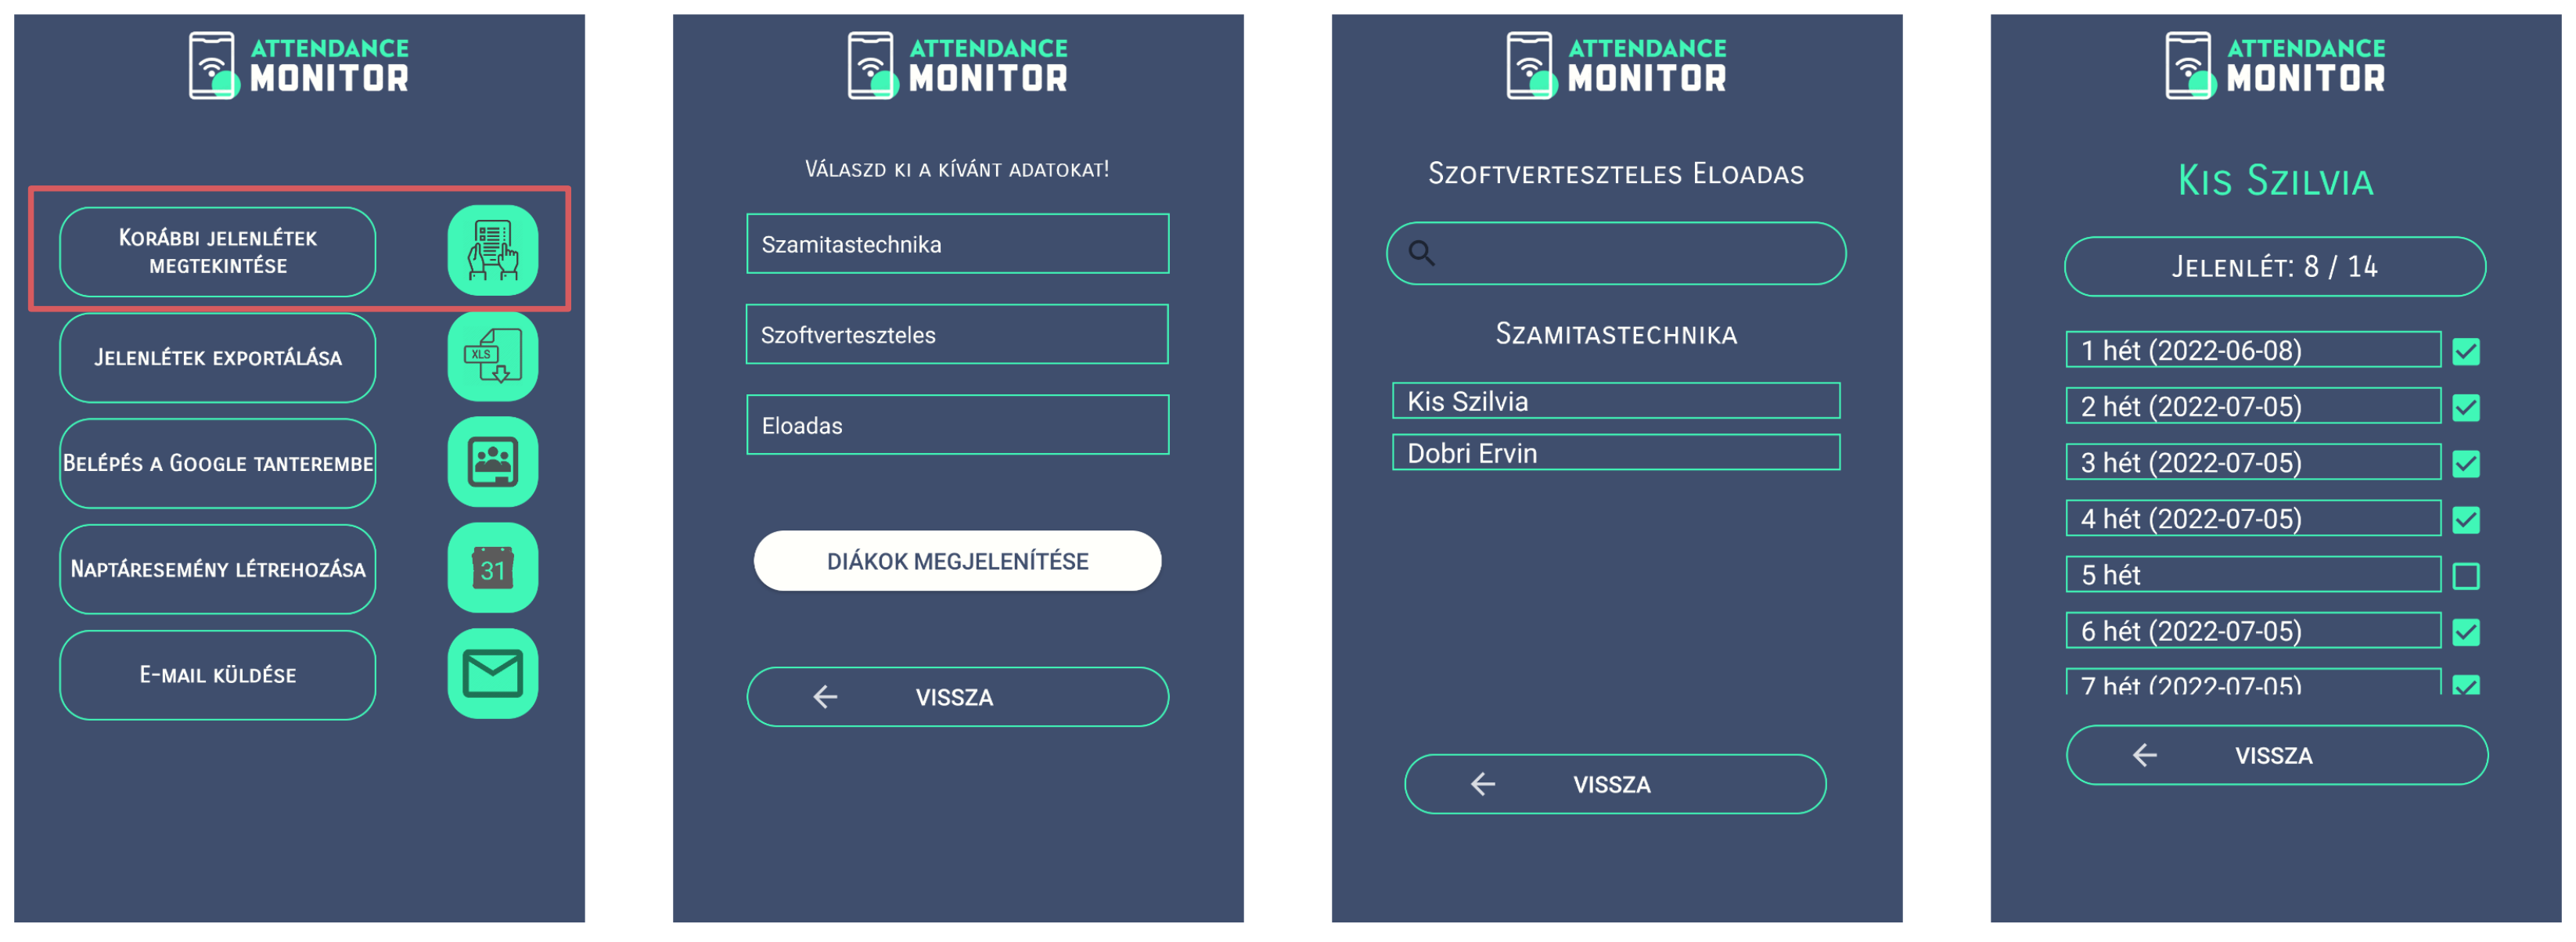
\includegraphics[width=\textwidth]{figures/gy5.png}
	\caption{Jelenlétek megtekintése a Tanár applikációban}
	\label{fig:gy5}
\end{figure}

\begin{figure}
	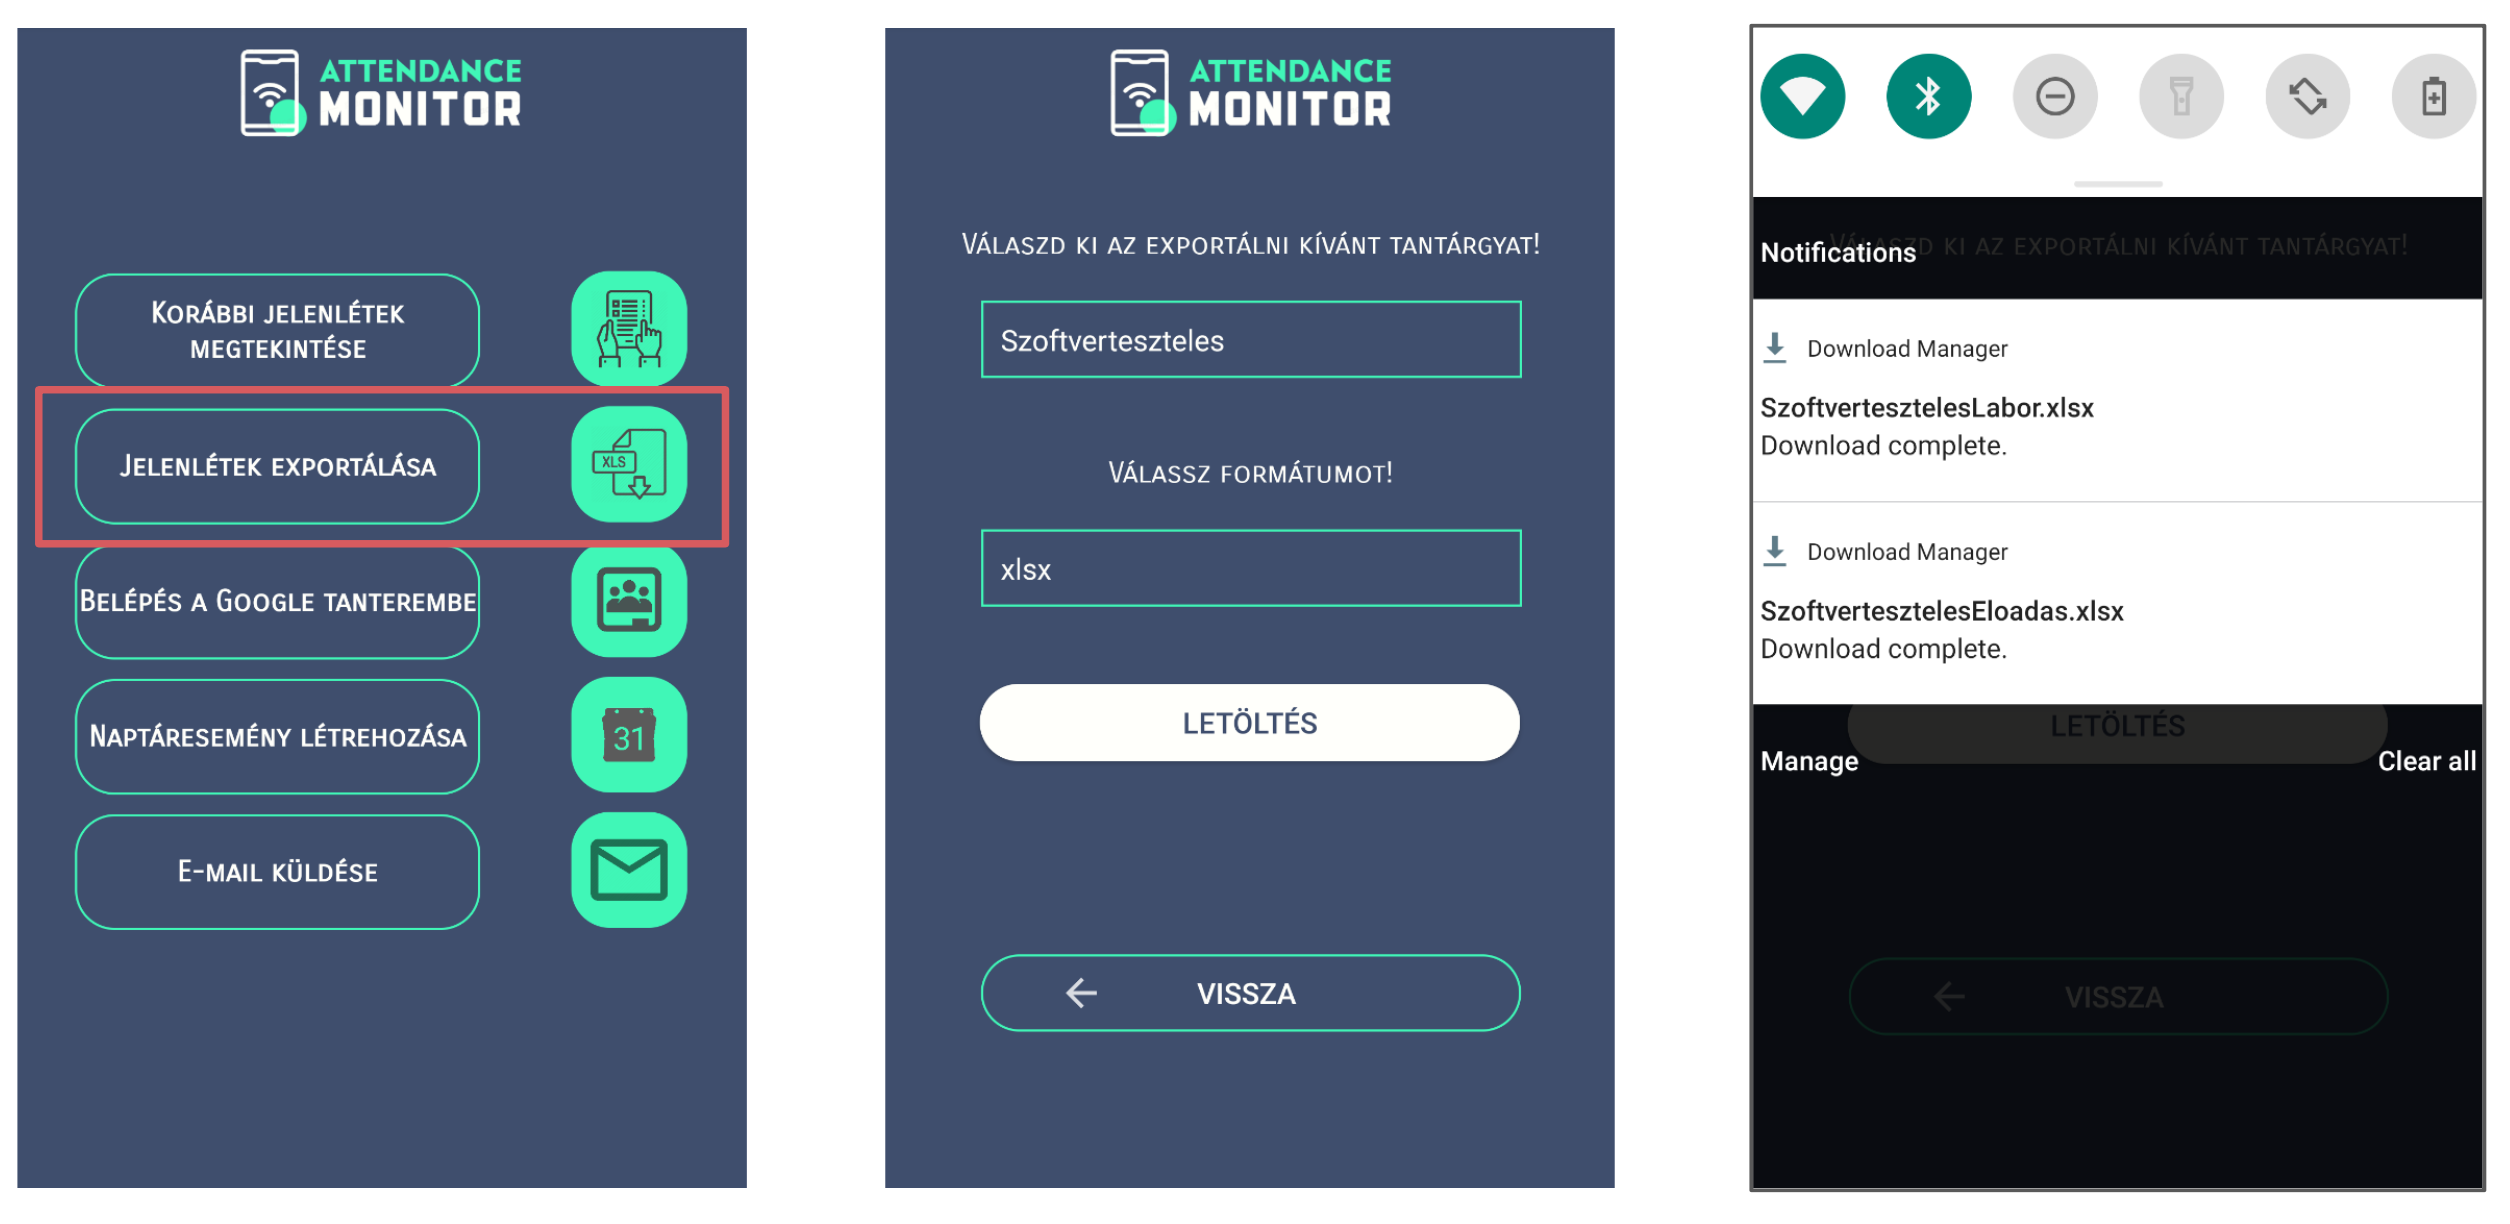
\includegraphics[width=\textwidth]{figures/gy6.png}
	\caption{Jelenlétek letöltése a Tanár applikációban}
	\label{fig:gy6}
\end{figure}

\begin{figure}
	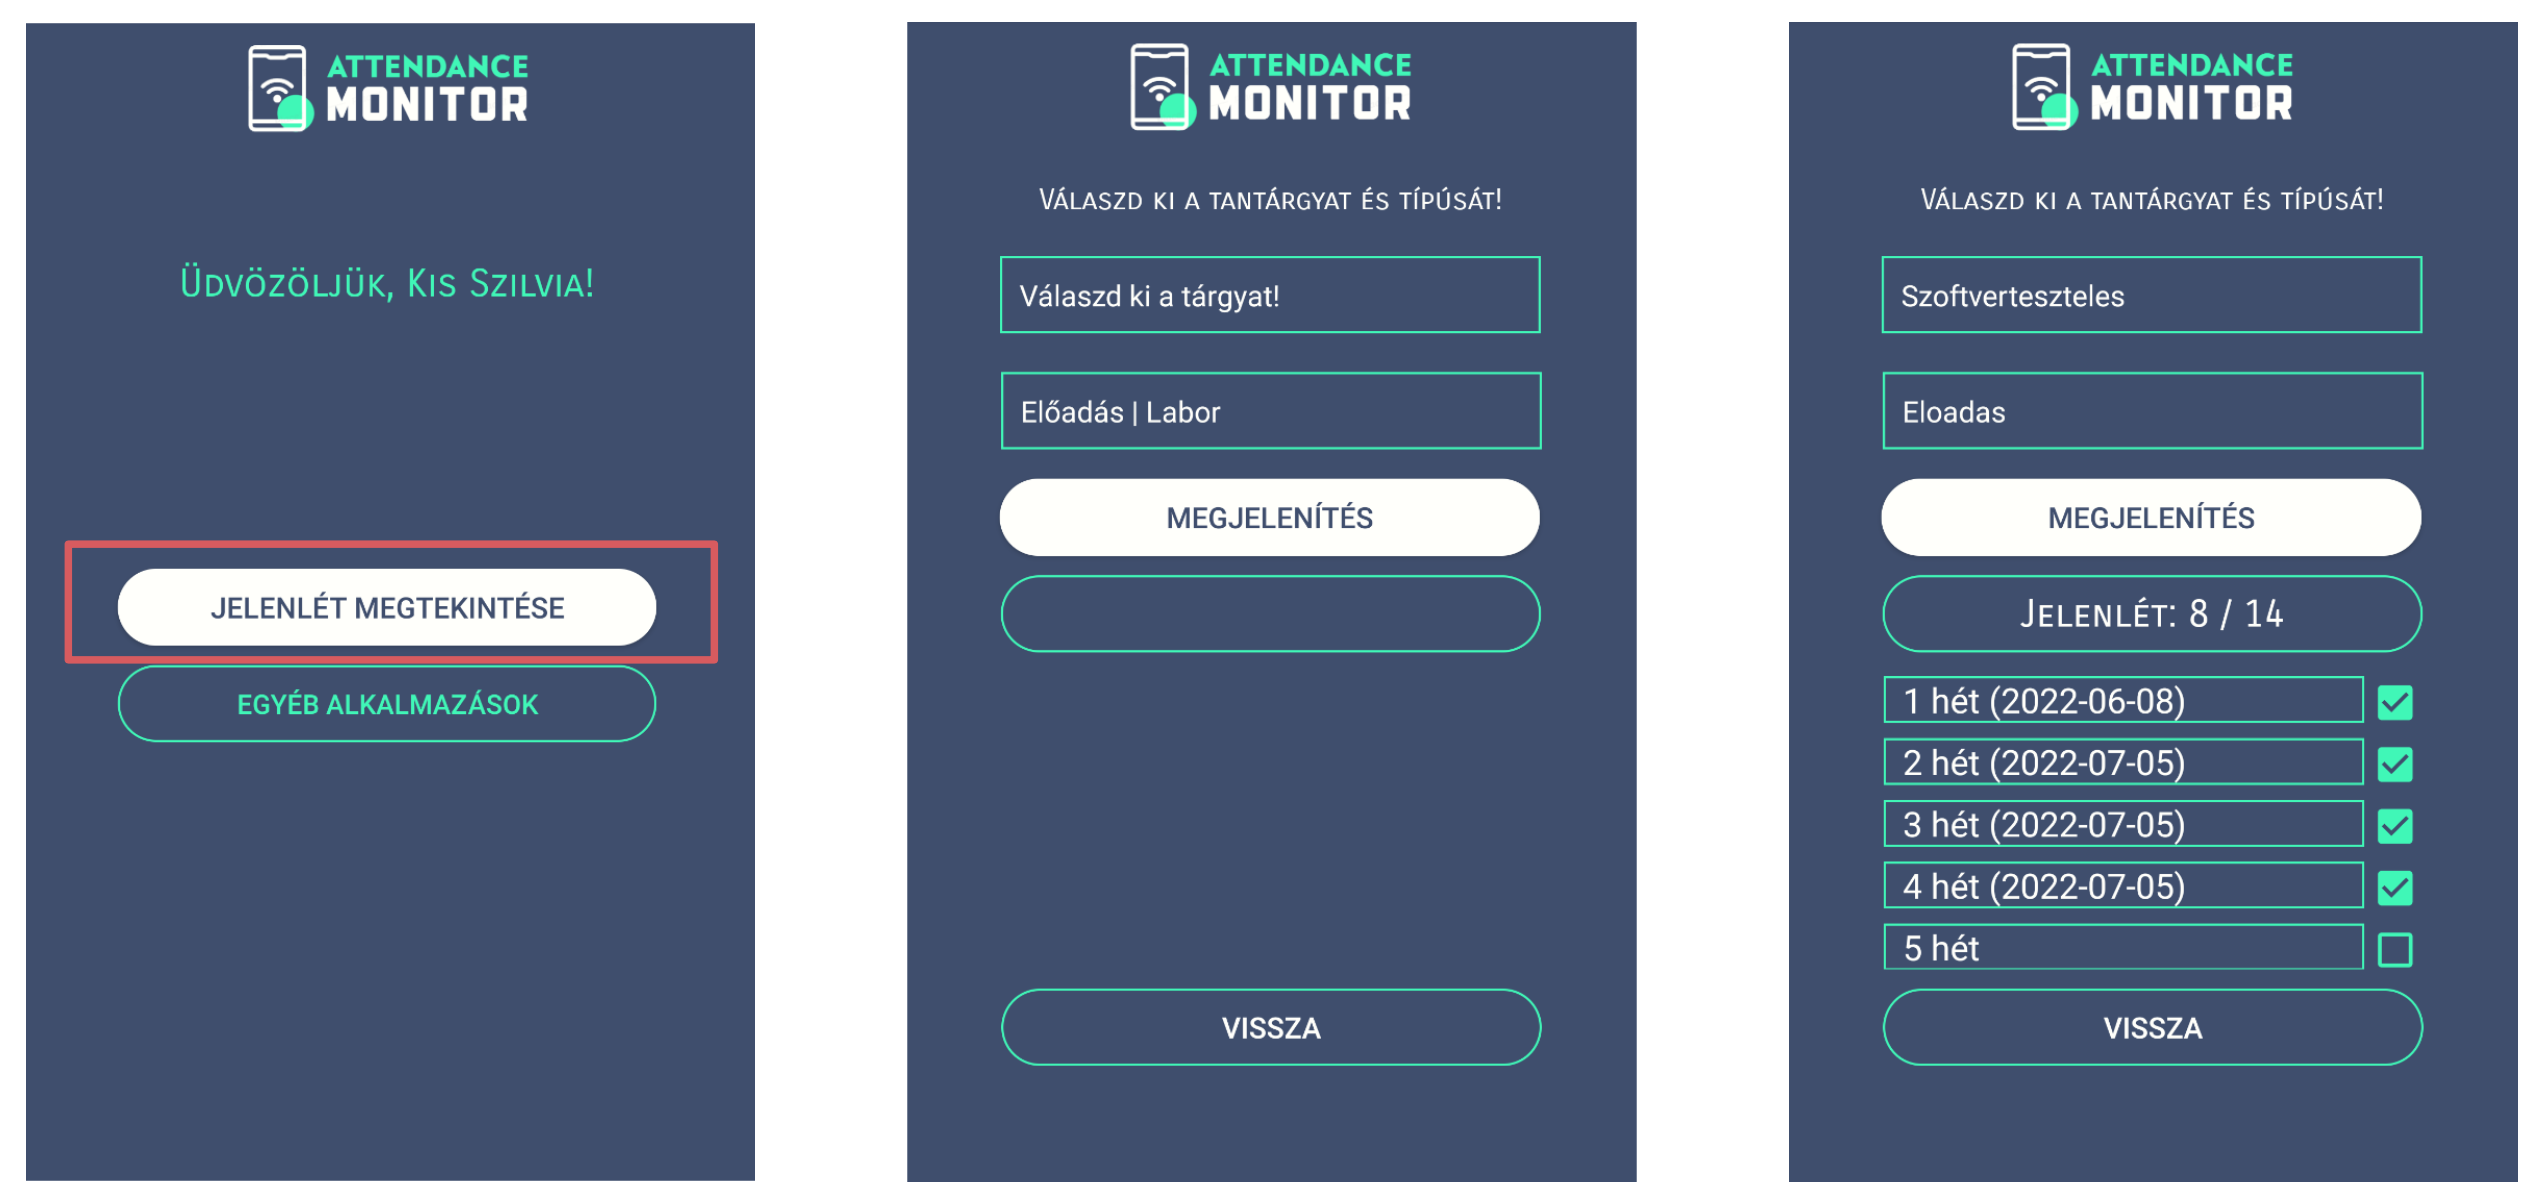
\includegraphics[width=\textwidth]{figures/gy7.png}
	\caption{Jelenlétek megtekintése a Diák applikációban}
	\label{fig:gy7}
\end{figure}
    %----------------------------------------------------------------------------
\chapter{Összefoglaló} \label{chapter9}
%----------------------------------------------------------------------------

A dolgozat során egy olyan szoftverrendszer kivitelezésére került sor, amely megpróbál eleget tenni a modernkori jelenlétkezelés elvárásainak, biztosítva a hatékony és megbízható működést, használata pedig az erre szánt időt minimálisra csökkenti, de ugyanakkor felhasználóbarát megjelenést kölcsönöz, mint a diák, mint pedig a tanárok számára.

Szoftverünk három fő modul köré épül. A diákok képeinek mentése és a jelenlétek bevitele az arcfelismerő és életszerűség-érzékelő modul részeit képezik. Ezáltal lehetőség van a fényképek egyszerű mentésére, valamint ami a legfontosabb, a jelenlétek gyors és biztonságos bevitelére. Emellett a Diák applikáció lehetővé teszi a hallgatók számára a jelenlétek utánkövetését, ugyanakkor e-mail küldését a tanárnak, valamint a Neptun és Google tanterembe való belépést is. A Tanár alkalmazásban is van lehetőség a korábbi jelenlétek megtekintésére, ezek kiexportálására több formátumban, illetve ugyanúgy vannak a kapcsolattartást elősegítő megoldások, mint például az e-mail küldés a diákoknak, naptáresemény létrehozása és kiküldése, valamint a Google tanterembe való belépés is adott. 

Amint azt a tapasztalataink is mutatják, fontos, hogy a folyamatok leegyszerűsítéséhez és felgyorsításához bátran használjuk az újszerű technológiákat, és haladjunk a modernizálás irányába. Ezáltal hatékonyabban és gyorsabban tudjuk elvégezni a repetitív munkákat és több idő marad azokra a dolgokra, amelyek a fejlődésünket szolgálják.

Összességében elmondhatjuk, hogy sikerült kivitelezni egy olyan élő arcfelismerés-alapú jelenlétkezelő alkalmazást, amely a robusztus működés mellett eleget tesz a 21. század technológiai elvárásainak, mindazonáltal egyszerűen kezelhető, mindenki számára elérhető, valamint nem igényel különleges szoftver és hardver készletet sem.

    %----------------------------------------------------------------------------
\chapter{Továbbfejlesztési lehetőségek} \label{chapter10}
%----------------------------------------------------------------------------

Bár igyekeztünk a rendszert a lehető legjobb formában kivitelezni, figyelembe véve a korábbi észrevételeket és javaslatokat, mégis vannak olyan hiányosságok, amelyeket a jövőben szeretnénk pótolni.

Ezek közül megemlíthetjük a következőket:

\begin{itemize}
    \item Mérések és kimutatások készítése a rendszer megbízhatóságáról.
    \item Platformfüggetlen mobil alkalmazások: a rendszer részét képező mobilapplikációk Flutterben való átírása.
    \item Diákok képeinek mentése adatbázisba.
    \item Párhuzamosítás: az arcfelismerő és életszerűség-érzékelő algoritmusok párhuzamos futásának megvalósítása.
    \item A jelenlétkezelő modul szinkronizálása a hivatalos órarenddel.
    \item Admin felület: az adatbázist kezelő adminisztrátor szerepkörű felhasználónak egy felhasználói felület létrehozása a feladatok megkönnyítése végett.
    
\end{itemize}

A következő tanévben szeretnénk tesztüzembe helyezni a jelenlétkezelő rendszert, majd egy felmérést végezni a felhasználók körében. A felmérés célja, hogy visszacsatolást kapjuk a rendszer használhatóságáról, esetleges hibáiról. Mindemellett pedig nyitottak vagyunk minden olyan javaslatra, amely segít, hogy az általunk megvalósított élő arcfelismerés-alapú jelenlétkezelő alkalmazás a lehető legideálisabb formát öltse.
%	\include{fejezet3}
%	\include{fejezet4}
%	\include{fejezet5}
%	\include{fejezet6}
%	\include{meresek}
%	\include{osszefoglalo}

% Koszonetnyilvanitas
%~~~~~~~~~~~~~~~~~~~~~~~~~~~~~~~~~~~~~~~~~~~~~~~~~~~~~~~~~~~~~~~~~~~~~~~~~~~~~~~~~~~~~~
%	\include{acknowledgement}


% Tablazatok es abrak jegyzeke (EZ NEM KOTELEZO)
%~~~~~~~~~~~~~~~~~~~~~~~~~~~~~~~~~~~~~~~~~~~~~~~~~~~~~~~~~~~~~~~~~~~~~~~~~~~~~~~~~~~~~~
	\listoffigures\addcontentsline{toc}{chapter}{\abrakjegyzeke}
%	\listoftables\addcontentsline{toc}{chapter}{\tablazatokjegyzeke}


% Bibliography
%~~~~~~~~~~~~~~~~~~~~~~~~~~~~~~~~~~~~~~~~~~~~~~~~~~~~~~~~~~~~~~~~~~~~~~~~~~~~~~~~~~~~~~
	\bibliography{mybib}
	\addcontentsline{toc}{chapter}{\irodalomjegyzek}
	\bibliographystyle{unsrt}
	
% Appendix
%~~~~~~~~~~~~~~~~~~~~~~~~~~~~~~~~~~~~~~~~~~~~~~~~~~~~~~~~~~~~~~~~~~~~~~~~~~~~~~~~~~~~~~
%	\include{appendices}

\label{page:last}
\end{document}
